% main.tex
% header.tex
\documentclass[a4paper,11pt,twoside,ngerman,color]{book}
\usepackage[a4paper,left=3.5cm,right=2.5cm,bottom=3.5cm,top=3cm]{geometry}

\usepackage[german,english]{babel}

\usepackage[pdftex]{graphicx,color}
\usepackage{amsmath,amssymb,subfigure}


% Theorem-Umgebungen
\usepackage[amsmath,thmmarks]{ntheorem}

% Korrekte Darstellung der Umlaute
\usepackage[utf8]{inputenc}
\usepackage[T1]{fontenc}

% mathematische Symbole
\usepackage{dsfont}

% Algorithmen
\usepackage{algorithmicx}
\usepackage[chapter]{algorithm}
\usepackage{algpseudocode}
\usepackage{listings}
\lstset{basicstyle=\ttfamily, breakatwhitespace=true, breaklines=true}

\usepackage{enumerate}

% Bibtex deutsch
\usepackage{bibgerm}
% \usepackage{biblatex}

% URLs
\usepackage{url}

% Caption Packet
\usepackage[margin=0pt,font=small,labelfont=bf]{caption}
% Gliederung einstellen
%\setcounter{secnumdepth}{5}
%\setcounter{tocdepth}{5}
\usepackage[breaklinks, pdftex]{hyperref} %hyperref still needs to be put at the end

% depth of numbering in sections
%\setcounter{secnumdepth}{3}

% Theorem-Optionen %
\theoremseparator{.}
\theoremstyle{change}
\newtheorem{theorem}{Theorem}[section]
\newtheorem{satz}[theorem]{Satz}
\newtheorem{lemma}[theorem]{Lemma}
\newtheorem{korollar}[theorem]{Korollar}
\newtheorem{proposition}[theorem]{Proposition}
% Ohne Numerierung
\theoremstyle{nonumberplain}
\renewtheorem{theorem*}{Theorem}
\renewtheorem{satz*}{Satz}
\renewtheorem{lemma*}{Lemma}
\renewtheorem{korollar*}{Korollar}
\renewtheorem{proposition*}{Proposition}
% Definitionen mit \upshape
\theorembodyfont{\upshape}
\theoremstyle{change}
\newtheorem{definition}[theorem]{Definition}
\theoremstyle{nonumberplain}
\renewtheorem{definition*}{Definition}
% Kursive Schrift
\theoremheaderfont{\itshape}
\newtheorem{notation}{Notation}
\newtheorem{konvention}{Konvention}
\newtheorem{bezeichnung}{Bezeichnung}
\theoremsymbol{\ensuremath{\Box}}
\newtheorem{beweis}{Beweis}
\theoremsymbol{}
\theoremstyle{change}
\theoremheaderfont{\bfseries}
\newtheorem{bemerkung}[theorem]{Bemerkung}
\newtheorem{beobachtung}[theorem]{Beobachtung}
\newtheorem{beispiel}[theorem]{Beispiel}
\newtheorem{problem}{Problem}
\theoremstyle{nonumberplain}
\renewtheorem{bemerkung*}{Bemerkung}
\renewtheorem{beispiel*}{Beispiel}
\renewtheorem{problem*}{Problem}

% Algorithmen anpassen %
\renewcommand{\algorithmicrequire}{\textit{Eingabe:}}
\renewcommand{\algorithmicensure}{\textit{Ausgabe:}}
\floatname{algorithm}{Algorithmus}
\renewcommand{\listalgorithmname}{Algorithmenverzeichnis}
\renewcommand{\algorithmiccomment}[1]{\color{grau}{// #1}}

% Zeilenabstand einstellen %
\renewcommand{\baselinestretch}{1.25}
% Floating-Umgebungen anpassen %
\renewcommand{\topfraction}{0.9}
\renewcommand{\bottomfraction}{0.8}
% Abkuerzungen richtig formatieren %
\usepackage{xspace}
\newcommand{\vgl}{vgl.\@\xspace} 
\newcommand{\zB}{z.\nolinebreak[4]\hspace{0.125em}\nolinebreak[4]B.\@\xspace}
\newcommand{\bzw}{bzw.\@\xspace}
\newcommand{\dahe}{d.\nolinebreak[4]\hspace{0.125em}h.\nolinebreak[4]\@\xspace}
\newcommand{\etc}{etc.\@\xspace}
\newcommand{\evtl}{evtl.\@\xspace}
\newcommand{\ggf}{ggf.\@\xspace}
\newcommand{\bzgl}{bzgl.\@\xspace}
\newcommand{\so}{s.\nolinebreak[4]\hspace{0.125em}\nolinebreak[4]o.\@\xspace}
\newcommand{\iA}{i.\nolinebreak[4]\hspace{0.125em}\nolinebreak[4]A.\@\xspace}
\newcommand{\sa}{s.\nolinebreak[4]\hspace{0.125em}\nolinebreak[4]a.\@\xspace}
\newcommand{\su}{s.\nolinebreak[4]\hspace{0.125em}\nolinebreak[4]u.\@\xspace}
\newcommand{\ua}{u.\nolinebreak[4]\hspace{0.125em}\nolinebreak[4]a.\@\xspace}
\newcommand{\og}{o.\nolinebreak[4]\hspace{0.125em}\nolinebreak[4]g.\@\xspace}
\newcommand{\oBdA}{o.\nolinebreak[4]\hspace{0.125em}\nolinebreak[4]B.\nolinebreak[4]\hspace{0.125em}d.\nolinebreak[4]\hspace{0.125em}A.\@\xspace}
\newcommand{\OBdA}{O.\nolinebreak[4]\hspace{0.125em}\nolinebreak[4]B.\nolinebreak[4]\hspace{0.125em}d.\nolinebreak[4]\hspace{0.125em}A.\@\xspace}

% Leere Seite ohne Seitennummer, naechste Seite rechts
\newcommand{\blankpage}{
 \clearpage{\pagestyle{empty}\cleardoublepage}
}

% Keine einzelnen Zeilen beim Anfang eines Abschnitts (Schusterjungen)
\clubpenalty = 10000
% Keine einzelnen Zeilen am Ende eines Abschnitts (Hurenkinder)
\widowpenalty = 10000 \displaywidowpenalty = 10000
% EOF

\begin{document}
\selectlanguage{german}
\begin{titlepage}
	\definecolor{TUGreen}{rgb}{0.517,0.721,0.094}
	\vspace*{-2cm}
	\newlength{\links}
	\setlength{\links}{-1.5cm}
	\sffamily
	\hspace*{\links}
	\begin{minipage}{12.5cm}
		
\includegraphics[width=8cm]{bilder/tud_logo_rgb}
		%\hspace*{-0.25cm} \textbf{TECHNISCHE UNIVERSIT"AT DORTMUND}\\
		%\hspace*{-1.2cm} \rule{5mm}{5mm} \hspace*{0.1cm} FACHBEREICH INFORMATIK\\
	\end{minipage}

	\vspace*{4.5cm}

	\hspace*{\links}
	\hspace*{-0.7cm}
	\begin{minipage}{17cm}
		\large	
		\begin{center}
			{\Large Bachelorarbeit} \\
			\vspace*{1cm}
			\textbf{Analyse von RAD-Seq-Daten als Optimierungsproblem unter  Berücksichtigung von Sequenzierfehler- und Mutationsraten} \\
			\vspace*{1cm}
			Antonie Vietor
			% \vspace*{1cm}
		\end{center}
	\end{minipage}
	\normalsize
	\vspace*{4.5cm}


	% \hspace*{\links}

	\vspace*{3.5cm}

	\hspace*{\links}
	\begin{minipage}[b]{8cm}
		% \normalsize
		\raggedright
		Gutachter: \\
		Name des Erstgutachters \\
		Name des Zweitgutachters \\
	\end{minipage}
	
	\vspace*{2.0cm}
	\hspace*{\links}
	\begin{minipage}[b]{8cm}
		% \normalsize
		\raggedright
		Technische Universit"at Dortmund \\
		Fakult"at f"ur Informatik\\
		Lehrstuhl 11 \\Bioinformatics for High-Throughput Technologies\\
		http://ls11-www.cs.tu-dortmund.de/
	\end{minipage}
		%%%%%%%%%%%%%%%%%%%%%%%%%%%%%%%%%%%%%%%%%%%%%%%%%%
		% bei Kooperation mit anderen Lehrstuehlen,
		% sonst weglassen
	\begin{minipage}[b]{8cm}
		% \normalsize
	\raggedleft
	In Kooperation mit:\\
	Universit"at Duisburg-Essen\\
	Genome Informatics\\
	http://genomeinformatics.uni-due.de/
	\end{minipage}
	%%%%%%%%%%%%%%%%%%%%%%%%%%%%%%%%%%%%%%%%%%%%%%%%%%
	
\end{titlepage}

\blankpage
\pagenumbering{roman}
\tableofcontents
\cleardoublepage
\pagenumbering{arabic}
% Kapitel
% einleitung.tex
\chapter{Einleitung} \label{sec:introduction}
\section{Biologischer Hintergrund} \label{sec:biology}
\subsection{Aufbau und Struktur der DNA} \label{subsec:dna}

% Eine Referenz~\cite{AggarwalV88}.

In den vergangenen Jahren wurden durch die molekulargenetische Methoden in Medizin und Biologie enorme Fortschritte erzielt. Heute sind sie nicht nur ein wesentliches Instrument bei der Erforschung, Diagnostik und Therapie verschiedenster Erkrankungen sondern sind auch bei der Entdeckung und Klassifikation von Organismen oder ganzen Ökosystemen von entscheidender Bedeutung.  \\

%\hyperlink{repl}{DNA-Replikation} 
%\hypertarget{repl}{DNA-Replikation}

Einer der ersten und wichtigsten Meilensteine auf dem noch eher jungen Gebiet der Molekulargenetik wurde $1953$ durch die Entdeckung der Doppelhelixstruktur der DNA und die Beschreibung ihres Aufbaus erreicht ~\cite{watson_1953}. Die DNA (desoxyribonucleic acid) ist ein langkettiges, aus zwei gegenläufigen, komplementären Strängen bestehendes und zu einer Helix gewundenes Molekül, welches die Erbinformation der meisten Zellen codiert. Die Komplementarität und Gegenläufigkeit werden in Kap. \ref{subsec:double_strand} gesondert beschrieben. Jeder Strang besteht aus vielen aneinandergereihten Nukleotiden, die sich jeweils aus einem Zuckermolekül (Desoxyribose), einem Phosphatrest und einer von vier möglichen Basen zusammensetzen. Als Basen kommen in der DNA Adenin (A), Thymin (T), Guanin (G) und Cytosin (C) vor. Die Kombinationen dieser Basen codieren über ihre Sequenz die genetische Information.  \\

Hierbei codieren im Rahmen der Proteinbiosynthese (Kap. \ref{subsec:protsynth}) Kombinationen aus jeweils drei Basen, sog. Basentripletts bzw. Codons, entweder für eine von i.d.R. $ 20 $ Aminosäure ~\cite{martin_1961, matthaei_1961} oder für Start- bzw. Stop-Sequenzen, welche den Anfang bzw. das Ende von Genen signalisieren (genetischer Code). Hiervon codieren $ 61 $ Tripletts für die bereits erwähnten $ 20 $ Aminosäuren. Somit codieren für die meisten Aminosäuren mehrere verschiedene Tripletts, diese Eigenschaft des genetischen Codes wird auch als Degeneration bezeichnet. \\

Die Basensequenz der DNA entspricht somit einer Aminosäuresequenz, welche die Primärstruktur von Proteinen (Eiweißmolekülen) darstellt. Proteine erfüllen in lebenden Organismen umfangreiche Funktionen, sie können als Hormone, Enzyme, Strukturproteine fungieren und sind an den meisten Stoffwechselprozessen und Signalwegen von Zellen beteiligt. Die verschiedenen Proteine werden jeweils von für sie spezifischen Abschnitten auf der DNA codiert. Solche DNA-Abschnitte werden als Gene bezeichnet. Ein DNA-Strang besteht aus vielen verschiedenen Genen. In komplexeren Zellen befinden sich im Zellkern in der Regel mehrere DNA-Stränge, die jeweils ein Chromosom repräsentieren, auf dem sich jeweils mehrere Gene befinden. Die Anzahl der Chromosomen innerhalb der Zellen ist speziesabhängig. \\

Zwischen den einzelnen Genen eines DNA-Stranges befinden sich nicht-codierende und oft repetitive Sequenzen. Ebenso gibt es auch innerhalb der Gene codierende Abschnitte (Exons) und nicht-codierende Sequenzen (Introns). Insgesamt machen die für Proteine codierenden Bereiche der DNA nur einen geringen Anteil des Genoms, also der gesamten Erbinformation einer Zelle aus. Beim Menschen wird dieser Anteil auf etwa $2$ \% geschätzt, d.h. ca. $ 98 $ \% des menschlichen Genoms besteht aus DNA, die nicht für Proteine codiert. Über diese nicht-codierenden Abschnitte ist bislang nur wenig bekannt, teilweise werden ihnen regulatorische Funktionen zugeschrieben ~\cite{dunham_2012, tsagakis_2020}. \\

\subsection{Bindungen innerhalb und zwischen DNA-Molekülen} \label{subsec:double_strand}
%Besonderheiten doppelsträngiger DNA

DNA liegt meist in Form eines Doppelstrangs vor. Die Basen beider Stränge sind dabei intermolekular über schwache chemische Bindungen, sogenannte Wasserstoffbrücken, mit einander verbunden. Dabei kann Adenin nur an Thymin unter Ausbildung von zwei Wasserstoffbrückenbindungen binden. Ebenso kann Cytosin nur mit Guanin über insgesamt drei Wasserstoffbrücken eine Bindung eingehen. Diese selektive Basenpaarung wird auch als Komplementarität bezeichnet. Es sind also Adenin und Thymin ebenso wie Cytosin und Guanin jeweils komplementär zu einander. Bezogen auf einen DNA-Doppelstrang sind auch seine beiden Einzelstränge komplementär, so das sich für jede Base des einen Stranges auf dem anderen Strang jeweils die komplementäre Base an der entsprechenden Position befindet. Es genügt also so die Sequenz von einem der beiden Stränge zu kennen, um die Sequenz des jeweils anderen rekonstruieren zu können. Dies wird sowohl zum Auslesen der genetischen Informationen bei der Transkription (Kap. \ref{subsec:transcription}) als auch zum Kopieren von DNA im Rahmen der DNA-Replikation (Kap. \ref{subsec:replication}) genutzt. \\

Wie bereits in Kap. \ref{subsec:dna} erwähnt, ist doppelsträngige DNA gegenläufig orientiert. Die Einzelstränge besitzen eine Polarität, welche durch die intramolekulare Bindung zwischen den einzelnen Nukleotiden über sogenannte Phosphodiesterbindungen zustande kommt. Dabei bindet der Phosphatrest, der sich jeweils am 5. Kohlenstoffatom (C5) des Zuckermoleküls der Nukleotide befindet, an das 3. Kohlenstoffatom (C3) des Zuckermoleküls des nachfolgenden Nukleotids. An den Enden eines DNA-Strangs fehlt jedoch diese Phosphodiesterbindung, so das an einem Ende das C3 ungebunden bleibt (3'-Ende) während am anderen Ende der Phosphatrest nur an C5 gebunden ist (5'-Ende) und somit die zweite Esterbindung am Phosphatrestes fehlt. Aufgrund der Gegenläufigkeit befindet sich also an beiden Enden eines Doppelstrangs jeweils ein 3'-Ende des einen und ein 5'-Ende des anderen Einzelstrangs. Diese Polarität spielt eine wichtige Rolle bei der Lese- und Synthese-Richtung im Rahmen der Transkription und der DNA-Replikation.\\

\subsection{RNA und die Proteinbiosynthese} \label{subsec:protsynth}

Ebenso wie DNA gehört auch RNA (ribonucleic acid) zu den Nukleinsäuren. Sie unterscheidet sich in ihrem Aufbau von der DNA durch die Base Uracil (U) statt Thymin und den Zucker Ribose statt Desoxyribose. Meist liegt RNA einzelsträngig oder nur über kürzere Abschnitte doppelsträngig vor. Während DNA insbesondere der Speicherung der Erbinformation dient, hat RNA eher die Funktion der Informationsübertragung. RNA nimmt daher zahlreiche regulatorische Funktionen war. \\

Eine ihrer wichtigsten Aufgaben ist die Übertragung der genetische Information von der DNA in die Aminosäuresequenz der Proteine bei der Proteinbiosynthese. Dabei werden von dem für das herzustellende Protein codierenden DNA-Abschnitt zunächst Arbeitskopien in Form von mRNA (messenger RNA) hergestellt. Ein solches Umschreiben von DNA in mRNA wird auch als Transkription bezeichnet. Nach der Transkription erhalten die mRNA-Fragmente noch einige Modifikationen und werden aus dem Zellkern hinaus in das Cytoplasma transportiert. Im Cytoplasma erfolgt schließlich mit Hilfe sogenannter tRNAs (transfer RNA) die Übersetzung der Basentripletts in eine Aminosäuresequenz (Translation, siehe auch Kap. \ref{subsec:dna}). tRNAs besitzen eine Bindungsstelle bestehend aus jeweils drei Nukleotiden, mit der sie komplementär an ein passendes Basentriplett der mRNA binden. In Abhängigkeit vom Basentriplett an ihrer mRNA-Bindungsstelle trägt jede tRNA entsprechend dem genetischen Code eine spezifischen Aminosäure. Entlang der mRNA wird nun ab der Startsequenz für jedes Basentriplett die passende tRNA nacheinander angelagert. Sobald eine tRNA bindet, wird die an sie gebundene Aminosäure gelöst und an die Aminosäure der nachfolgenden tRNA gebunden. Dadurch entsteht eine Kette von aneinander gebundene Aminosäuren, die sich jeweils entsprechend der mRNA Sequenz an die Aminosäure der nächsten passenden tRNA anlagert und um deren Aminosäure verlängert. Beim Erreichen einer Stop-Sequenz kann diese keine tRNA angelagern, die Synthese wird abgebrochen und die Aminosäurekette löst sich von der zuletzt gebundenen tRNA und wird weiteren Modifikationen unterzogen. \\

\subsection{DNA-Replikation} \label{subsec:replication}

Die DNA-Replikation dient der Verdopplung der DNA im Rahmen der Zellteilung, so dass jede der beiden resultierenden Tochterzellen das gleiche genetische Material erhält. Die DNA-Replikation ist also ein natürlicher Vorgang zur Erzeugung von DNA-Kopien. Ihr grundlegendes Prinzip findet bei der PCR (Polymerase-Ketten-Reaktion, siehe Kap. \ref{subsec:pcr}) Anwendung und wird für verschiedene molekulargenetische Verfahren genutzt, um DNA-Kopien synthetisch herzustellen. In diesem Zusammenhang sei hier auf die verschiedenen Sequenzierungstechniken insbesondere im Hinblick auf das RAD-Sequencing verwiesen (Kap. \ref{subsec:sanger}, Kap. \ref{subsec:ngs} und Kap. \ref{sec:rad}). Daher soll der Vorgang der DNA-Replikation im Folgenden kurz umrissen werden ~\cite{odonell_2013, chargin_2010, prioleau_2016}. \\

Bei eukaryotischen Zellen, die im Gegensatz zu Bakterien (Prokaryoten) einen Zellkern besitzen, liegt die DNA im Zellkern häufig gewunden und stark kondensiert vor. Um ihre Sequenz Base für Base kopieren zu können, muss sie zunächst entwunden werden. Dies geschieht durch Enzyme aus der Gruppe der Topoisomerasen. Diese erzeugen gezielt am Replikationsursprung temporäre Strangbrüche in der DNA und entspannen so den Doppelstrang. Anschließend setzt am Replikationsursprung ein weiteres Enzym, die Helikase, an und trennt die beiden komplementären Stränge auf. Es entsteht die sogenannte Replikationsgabel. Während der Replikation schiebt sich die Helikase unter fortlaufender Auftrennung der beiden Stränge auf der DNA entlang. Auch bei diesem Prozess sorgen Topoisomerasen immer wieder für eine Entspannung des DNA-Fadens hinsichtlich seiner Windung. \\

Nun kann der eigentliche Kopiervorgang an den beiden von einander getrennten Einzelsträngen mit Hilfe von DNA-Polymerasen erfolgen. Dabei fahren die DNA-Polymerasen an den Strängen entlang und fügen an jeder Position des Elternstranges Nukleotide mit der jeweils komplementären Base an. Im Ergebnis entsteht also an jedem der beiden Elternstränge ein neuer komplementärer DNA-Strang, der also die gleiche Basensequenz wie der jeweils andere Elternstrang besitzt. Bei den DNA-Polymerasen handelt es sich um Enzyme, die für die Initiation des Kopiervorgangs eine Startsequenz benötigen. Diese Startsequenzen sind kleine RNA-Fragmente mit spezifischer Basensequenz, die sich an die jeweils passende, komplementäre Stelle auf dem Elternstrang anlagern. An diese, auch als RNA-Primer bezeichneten Fragmente kann nun die DNA-Polymerase binden und mit der Replikation beginnen. \\

Die DNA-Polymerase kann den Elternstrang nur in eine Richtung lesen, nämlich vom 3' Ende zum 5' Ende (3'-5'-Richtung). Aufgrund der gegenläufigen, antiparallelen Ausrichtung zweier komplementärer Stränge zu einander, kann folglich die Synthese des Tochterstranges nur in 5'-3'-Richtung erfolgen. Für die beiden antiparallel ausgerichteten Elternstränge bedeutet dies, dass nur bei einem Strang die Richtung der sich öffnenden Replikationsgabel der 5'-3'-Richtung des Stranges entspricht. Dieser Strang kann kontinuierlich repliziert werden, da sich die DNA-Polymerase auf ihm in Richtung der voranschreitenden Aufspaltung des Doppelstranges bewegt. Der auf diese Weise kontinuierlich synthetisierte Strang wird als Leitstrang bezeichnet. \\

Der andere Strang ist jedoch in Gegenrichtung orientiert, so dass seine Syntheserichtung, also die 5'-3'-Richtung, entgegengesetzt zur Bewegungsrichtung der Replikationsgabel orientiert ist. Dadurch können jeweils nur kleinere Fragmente synthetisiert werden die von der Replikationsgabel bis zum bereits replizierten Teil des Strangs reichen. Schreitet die Öffnung der Replikationsgabe weiter fort, muss der nun frei gewordene Strangabschnitt ebenfalls synthetisiert werden. Es muss also erneut ein RNA-Primer angelagert werden und dann mit Hilfe der DNA-Polymerase der Bereich zwischen Replikationsgabel und bereits replizierten Strang synthetisiert werden. Die Replikation erfolgt somit diskontinuierlich. Der so synthetisierte Strang wird als Folgestrang bezeichnet und besteht zunächst aus multiplen Fragmenten (Okazaki-Fragmente). Nach dem Replikationsvorgang werden mit Hilfe der DNA-Polymerase die RNA-Primer durch DNA ersetzt. Im Anschluss werden die multiplen Fragmente des Folgestrangs durch Ligasen zu einem kontinuierlichen Strang verbunden. Im Ergebnis sind also nach Abschluss der DNA-Replikation zwei identische Kopien der beiden Elternstränge entstanden.\\

\subsection{Mutationen und SNPs} \label{subsec:mutation}

Veränderungen in der DNA-Sequenz werden als Mutationen bezeichnet. Sie können durch zellinterne Faktoren verursacht werden, wie beispielsweise Fehler beim Kopiervorgang der DNA (DNA-Replikation) während der Zellteilung. Ebenso können sie durch zahlreiche Umwelteinflüsse entstehen. \\

Mutationen können unterschiedlich große Abschnitte der DNA betreffen, von ganzen Chromosomen oder großen Chromosomenabschnitten über Veränderungen von mehreren Basen bis hin zu sogenannten Punktmutationen, bei denen nur eine einzige Base verändert ist. Auf DNA-Ebene können Punktmutationen in Form Substitutionen, Insertionen und Deletionen auftreten. Bei der Substitution wird eine Base durch eine andere ausgetauscht, bei der Insertion wird eine zusätzliche Base in den DNA-Strang eingefügt und bei der Deletion kommt es zum Verlust einer Base. \\

Liegt eine solche Punktmutation in den codierenden DNA-Abschnitten, so können sich auf Proteinebene verschiedene Konsequenzen daraus ergeben. Punktmutationen in Form von Insertionen bzw. Deletionen bewirken durch die zusätzliche bzw. fehlende Base eine Verschiebung des Leserasters, so dass sich die Triplettstruktur für alle nachfolgenden Basen verschiebt. Dies wird als Frame-Shift bezeichnet und verursacht meist eine gravierende Veränderung des resultierenden Proteins, da viele der nachfolgenden Tripletts nun für andere Aminosäuren codieren. Dies führt häufig zu einem deutlich veränderten Protein, welches seine reguläre Funktion nicht mehr oder nur noch unvollständig wahrnehmen kann. Auch bei Insertionen und Deletionen von mehreren Basen kann es zu einem Frame-Shift kommen, sind allerdings drei Basen oder ein Vielfaches hiervon betroffen, so bleibt das Leseraster erhalten.  \\

Bei Substitutionen bleibt dagegen das Leseraster erhalten. Aufgrund der Degeneration des genetischen Codes können verschiedene Basentripletts für die gleiche Aminosäure codieren. Dadurch kann ein Basentriplett mit einer Punktmutation trotz des Basenaustauschs noch für die ursprüngliche Aminosäure codieren, so dass das resultierende Protein unverändert bleibt. In diesem Fall spricht man von einer silent-Mutation. Codiert das Basentriplett aber aufgrund der Mutation für eine andere Aminosäure, so handelt es sich um eine missense-Mutation. Die Proteinsequenz wird dadurch in einer Aminosäure geändert, so dass es je nach Position der betreffenden Aminosäure zu verschieden starken Effekten hinsichtlich der Proteinfunktion kommen kann. \\

Zudem können Substitutionen und Frame-Shifts dazu führen, dass ein für eine Aminosäure codierendes Basentriplett zu einem Stop-Codon umgewandelt wird (nonsense-Mutation) oder ein Stop-Codon durch die Mutation für eine Aminosäure codiert (readtrough-Mutation). \\

Hinsichtlich der Eigenschaften des resultierenden Proteins unterscheidet man im Zusammenhang mit Mutationen zudem zwischen sogenannten loss-of-function- und gain-of-function-Mutationen. Loss-of-function-Mutationen führen zu einer verringerten Funktionalität oder dem vollständigen Funktionsverlust des Proteins. Gain-of-function-Mutationen bewirken dagegen eine verstärkte oder veränderte Aktivität bzw. Funktionalität des Proteins. \\

Wie bereits erwähnt führen aber nicht alle Veränderungen der DNA-Sequenz zu Störungen der Genfunktion. Veränderungen ohne unmittelbaren Krankheitswert werden als genetische Varianten bezeichnet, wenn sie innerhalb einer Spezies vermehrt auftreten ~\cite{vignal_2002, sachidanandam_2001}. Am häufigsten finden sich dabei Varianten einzelner Basenpaare, sogenannte SNP‘s (single nucleotide polymorphisms). SNP‘s kommen sowohl in codierenden als auch nicht-codierenden DNA-Abschnitten vor und treten regionsabhängig in unterschiedliche Häufigkeit auf. SNP‘s können als genetische Marker benutzt werden ~\cite{kruglyak_1997, kwok_2003}, ihr Auftreten und ihre Verteilung spielen vor allem in der Populationsgenetik eine wichtige Rolle. Sie können Aufschluss hinsichtlich der Diversität, Selektion und Demographie einer Population geben ~\cite{nielsen_2004, shriver_2004, akey_2002}. \\

Während große strukturelle Chromosomenaberrationen unter Umständen bereits lichtmikroskopisch erkennbar sind, ist bei Punktmutationen oder SNP‘s lediglich eine einzige Base verändert. Solche Veränderungen lassen durch verschiedene molekulargenetische Verfahren detektieren ~\cite{kwok_2003, wang_1998}. Insbesondere die direkte Analyse der DNA-Sequenz mittels Sequenzierung  (siehe Kap. \ref{subsec:sanger}) ist durch die Entwicklung der sogenannten Next-Generation-Sequenzing-Verfahren (NGS) im Hochdurchsatzverfahren und mit hoher Parallelisierung durchführbar (siehe Kap. \ref{subsec:ngs}). Diese Techniken ermöglichen inzwischen umfangreiche, genomweite Analysen hinsichtlich einer großen Vielfalt molekulargenetischer Fragestellungen. Die vorliegende Arbeit befasst sich mit der Analyse und Auswertung von RAD-Sequencing-Daten. Auch die RAD-Sequenzierung gehört zu den NGS-Verfahren und dient insbesondere der Detektion von SNPs. Daher wird dieses Verfahren in Kap. \ref{sec:rad} detaillierter vorgestellt.\\

\section{Molekulargenetische Verfahren und Techniken} \label{sec:methods}
\subsection{Sanger-Sequenzierung} \label{subsec:sanger}

Nach der Erforschung der DNA-Struktur war schließlich die Entwicklung der Sanger-Sequenzierung im Jahr $1975$ ein entscheidender Meilenstein der molekulargenetischen Forschung ~\cite{sanger_1975}. Durch sie war es erstmals möglich die genaue Basensequenz eines DNA-Strangs zu bestimmen. \\

Hierbei wird die zu sequenzierende DNA-Probe in vier Teile aufgeteilt, denen jeweils eine der vier DNA-Basen in Form von radioaktiv markierten synthetischen Nukleotiden, sowie anteilig einige modifizierte Nukleotiden dieser Base hinzugefügt werden. Die jeweils anderen drei Basen werden als unmarkierte und unmodifizierte Nukleotide hinzugegeben. In jeder der Probengemische ist also eine andere Base markiert und zum Teil auch modifiziert. \\

Wie bei der natürlichen DNA-Replikation (siehe Kap. \ref{subsec:replication}) während der Zellteilung kann die Proben-DNA durch Hinzugabe der DNA-Polymerase I kopiert werden. Dabei werden auch die radioaktiv markierten Nukleotide in den kopierten Strang eingebaut. Die Kopiervorgänge starten jeweils an einem kleinen Fragment mit bekannter DNA-Sequenz, dem sog. Primer. Auch die Primer werden vorab den Probengemischen beigefügt. Der Primer bindet komplementär an die Ausgangs-DNA der Probe und  ermöglicht dadurch schließlich die Bindung der DNA-Polymerase. Diese fährt vom Primer aus am Ausgangsstrang entlang und fügt dabei zu jeder Base des Ausgangsstrangs ein Nukleotid mit komplementärer Base an die Kopie an. Wird dabei eines der modifizierten Nukleotide eingefügt, so kann im nächsten Schritt kein weiteres Nukleotid mehr an den kopierten Strang angefügt werden und der Synthesevorgang wird abgebrochen. Dadurch entstehen multiple, radioaktiv markierte DNA-Fragmente unterschiedlicher Länge. In jedem der Probenansätze enden diese Fragmente mit der selben Base, da nur eine der vier Basen in modifizierter Form hinzugegeben wurde. \\

Die vier Proben werden nun nebeneinander auf ein Gel aufgetragen. Da DNA negativ geladen ist bewegt sie sich im elektrischen Feld zur Anode. Wird also an das Gel ein elektrisches Feld angelegt, so werden die DNA-Fragmente durch das Gel bewegt. Kleinere Fragmente werden dabei schneller bewegt als größeren. Dadurch ist es möglich die DNA-Fragmente der Proben entsprechend ihrer Länge aufzutrennen. Es entstehen im Gel Anhäufungen von Fragmenten gleicher Länge, die auch als Banden bezeichnet werden. Die radioaktive Markierung der Banden kann auf Röntgenfolie sichtbar gemacht werden. Bei moderneren Verfahren ist die Markierung mit radioaktiven Isotopen durch Fluoreszenzfarbstoffe abgelöst worden. Da bekannt ist in welchen Proben welche der Basen markiert ist, kann die DNA-Sequenz direkt aus der aufsteigenden Länge der DNA-Fragmente an den Banden abgelesen werden. \\

\subsection{PCR}  \label{subsec:pcr}

Zunächst waren für die Sanger-Sequenzierung große Mengen an Zellmaterial notwendig, um daraus ausreichend DNA für sichtbare Banden auf dem Gel extrahieren zu können. Die Sequenzierung mit nur geringen DNA-Mengen war nicht möglich. Durch die Entwicklung des Verfahrens der Polymerasekettenreaktion (PCR, polymerase chain reaction) ~\cite{mullis_1986} wurden die Möglichkeiten der Sequenzierung revolutioniert. Die PCR ermöglicht es aus kleinsten DNA-Proben multiple Kopien herzustellen. Und so ist es inzwischen möglich, selbst aus der DNA einer einzigen Zelle umfangreiche Analysen durchzuführen ~\cite{gawad_2016}. \\

%PCR und Human genome project ~\cite{mcpherson_2001}


\subsection{Next Generation Sequencing} \label{subsec:ngs}
%Parallelisierung
%kostengünstig 
%highthroughput

\section{RAD-Sequencing} \label{sec:rad}

%genotypisierung, evolution, öklologie, genotyp/phenotyp, populationsgenetik, diversität, molekulare Ökologie, systematiken
%
%gleichzeitige Sequenzierung multipler Genomabschnitte (DNA)
%Detektion von SNPs 
%Restriktionsenzyme Restriction Endonucleases
%Restriktionsstellen bei verwandten Arten sehr ähnlich => ermöglicht Sequenzierung vergleichbarer/ähnlicher Abschnitte des Genoms zw. verwanden Arten
%ein oder mehrere Restriktionsenzyme
%
%Adapter + Barcode (Proben-ID, ist eine Sequenz), alle Amplifikate der Probe besitzen diese ID-Sequenz → können der Probe zugeordnet werden
%
%intra- und interspeziesvergleich dadurch möglich, Vergleich zwischen Individuen, ohne ihr gesamtes Genom zu sequenzieren möglich
%
%mehrere 100 Proben, 100-tausende loci genomweit und random => Flexibilität der Marker und ihrer Anzahl
%
%mehrere Proben werden gepoolt und dann sequenziert
%die sequenzierten Abschnitte (ab Restriktionsstelle) sind ca. 100-150 bp lang
%
%bei NGS wird jeder dieser Abschnitte mehrfach sequenziert => von jedem Abschnitt werden multiple, identische Fragmente (Reads) 
%
%Aufbau: Restriktionsstelle – Barcode – ca. 100 bp Sequenzinformation
%Loci werden anhand der Reads bestimmt, SNPs werden den Reads durch Clustering zugeordnet, Barcode ordnet die Proben den Reads und ihren SNPs zu
%
%=> Ergebnis: mehrere Milionen dieser Fragmente 
%
%
%
%Reference-free SNP Detection ~\cite{leggett_2014}.

\section{Sequenzierungsdaten und -formate}
\subsection{Reads} \label{subsec:fastq}
Identifikationsbezeichnungen, der Basensequenz, Basenqualität 

\subsection{Sequenzalignments} \label{subsec:samformat}

Häufig werden für die Analyse von Sequenzierungsdaten sogenannte Alignments erstellt, bei denen eine Readsequenz (Query) gegen eine andere Sequenz (Reference) verglichen wird. In Abhängigkeit von ihren Übereinstimmungen (Matches) und Unterschieden (Mismatches) werden die Sequenzen einander zugeordnet. Ein solches Alignment im SAM/BAM-Format wird auch in der vorliegenden Arbeit zur weiterführenden Analyse verwendet. \\

Das SAM/BAM-Format ~\cite{li_2009} enthält unter anderem die ID's der Query- und Reference-Sequenzen, Informationen zur Basenqualität, Readlänge und -sequenz, den sogenannten CIGAR-String sowie verschiedene optionale Tags, wie beispielsweise den NM-Tag, der die Edit-Distanz angibt (vgl. Kap. \ref{subsec:sol_graph}). Die Edit-Distanz ist die mindestens notwendige Anzahl von Ersetzungs-, Einfügungs- und Löschungsoperationen, um die Sequenz des Source-Knotens in die Sequenz des Target-Knotens zu transformieren. Auf DNA-Ebene entspricht dies den Punktmutationen im Sinne von Substitutionen, Insertionen und Deletionen (vgl. Kap. \ref{subsec:mutation}). Der CIGAR-String hingegen ist eine kondensierte Darstellung der Unterschiede zwischen Query- und Reference-Sequenz. In im SAM-Format werden darin Matches mit $ M $ oder $ = $, Mismatches mit $ X $  oder $ S $,  Insertionen mit $ I $ und Deletionen mit $ D $ sowie jeweils mit der Anzahl der betroffenen Basen codiert (siehe auch Kap. \ref{subsec:mutation}). Aus ihrer Summe mit Ausnahme und abzüglich der Deletionen ergibt die Readlänge. So ergibt beispielsweise der CIGAR-String $ 69=1X24= $ ein Matching der ersten $ 69 $ Basen des Queryreads beim Abgleich mit dem Referenzread, anschließend ist bei einer Base ein Mismatch aufgetreten und schließlich folgen $ 24 $ Basen die auf den Referenzread matchen. Die Readlänge beträgt somit insgesamt $ 94 $ Basen und die Edit-Distanz im NM-Tag besitzt den Wert $ 1 $. \\

Daneben gibt es weitere Darstellungsmöglichkeiten von Veränderungen der Querysequenz gegenüber der Referenzsequenz. So können im cs-Tag des SAM-Formats verkürzt (short) oder vollständig mit Angabe der gesamten Readsequenz die genauen Veränderungen mit Bezeichnung der betreffenden Basen angegeben werden. Bezüglich des oben genannten Beispiels kann der dazugehörige short cs-Tag $ 69*tc:24 $ lauten und zeigt damit an, dass nach Base $69$ ein Basenaustausch von Thymin gegen Cytosin erfolgt ist.
\subsection{Varianten} \label{subsec:vcf}

% kapitel2.tex
\definecolor{light-gray}{gray}{0.93}
\chapter{Analyse von RAD-Seq-Daten} \label{chapter:kap2}
\section{Problemstellung} \label{sec:probl}

Ausgangsmaterial für RAD-Seq-Analysen sind die Reads aus in der Regel gepoolten Probengemischen mehrerer Individuen. Durch entsprechende Barcodemarkierungen können die Reads den einzelnen Individuen zugeordnet werden. Durch die Verwendung gepoolter Probengemischen ist das Verfahren kostengünstiger und zeitsparender als die meisten anderen NGS-Verfahren. Die Reads stammen aus dem gesamten Genom, wobei sie nur kleinere Sequenzabschnitte zwischen den Schnittstellen der Restriktionsenzyme repräsentieren und damit nicht das gesamte Genom abbilden. Ein deutlicher Vorteil des Verfahrens besteht darin, die Reads ohne Kenntnis eines Referenzgenoms möglichen Loci zuordnen zu können. Auch die Loci und ihre Sequenz sind somit anfangs unbekannt und werden erst durch die Analyse ermittelt.\\

Das RAD-Sequencing-Verfahren bedingt, dass durch die Restriktionsenzyme die DNA nur in innerhalb spezifischer Sequenzen geschnitten wird und dass durch PCR und Sequenzierung mehrere Reads erzeugt werden, die jeweils vom gleichen Locus stammen. Das hier implementierte Tool NodeRAD stellt einen Prototypen dar, der im Gegensatz zu derzeit etablierten RADSeq-Tools, wie beispielsweise dem Tool Stacks \cite{catchen_2013}, mit Hilfe von nur zwei Parametern diese Zuordnung realisiert. Das Clustering der Reads sowie die Identifizierung und Locizuordnung sollen dabei unter Berücksichtigung der Ploidie ohne weiteres Vorwissen allein auf Grundlage der Sequenzierfehlerrate und Heterozygotiewahrscheinlichkeit erfolgen. Die ermittelten Loci sollen für anschließende Diversitätsanalysen zur Verfügung stehen. 

\section{Formale Definition der Problemstellung} \label{sec:formal}

Gegeben sei eine Menge von Reads eines Individuums $ D = (s_{1}, \dots , s_{m}) \in \{A,\,C,\,G,\,T,\}^{k^m}$ mit der Readlänge $k$. In den Reads sind zudem für jede Base Informationen zur Qualität der Sequenzierung $ Q = (q_{1}, \dots , q_{m}) \in {[0,\,1]}^{k^m}$ enthalten. Weiterhin seien für Substitutionen, Insertionen und Deletionen die Heterozygotiewahrscheinlichkeit $\eta = (\eta_{sub},\, \eta_{ins},\, \eta_{del}) $ und für Indels die Sequenzierfehlerrate $\epsilon=(\epsilon_{ins},\, \epsilon_{del})$ gegeben. Ebenso ist die Ploidie $\phi$ des untersuchten Organismus bekannt. In der vorliegenden Arbeit wird im Model und beim implementierten Prototypen ein diploider Chromosomensatz vorausgesetzt, für höherploide Organismen ist eine Anpassung hinsichtlich des Sequenzalignments notwendig (siehe Kap. \ref{sec:ausblick}). \\

Ziel ist die Zuordnung der Reads zu den Loci unter Berücksichtigung von $\epsilon$ und $\eta$ sowie die Ausgabe der Menge der ermittelten Loci mit den Sequenzen der beteiligten Allele. Dabei soll die Menge von Loci gefunden werden, welche die beobachteten Reads am besten erklären kann, das heißt welche die höchste Wahrscheinlichkeit in Zusammenschau mit $\epsilon$ und $\eta$ besitzt. \\

\section{Lösungsansatz und Modell} \label{sec:solution}

Das Problem wird als gerichteter Graph betrachtet (siehe Kap. \ref{subsec:sol_graph}), dessen Knoten die einzelnen Reads beinhalten und dessen Kanten auf einem Sequenzalignment der Reads basieren. Für die Zuordnung der Reads soll das Problem in Teilprobleme aufgeteilt werden, für jedes Teilproblem wird dann eine Lösung ermittelt. Der Graph wird daher entsprechend seiner Zusammenhangskomponenten partitioniert. Die in einer Zusammenhangskomponente vorkommenden Sequenzen werden in Abhängigkeit von festgelegten Schwellwerten als Kandidatenallele betrachtet und jeweils mit sämtlichen Reads der Zusammenhangskomponente verglichen. Dabei sollen diejenigen Allele identifiziert werden, von denen die übrigen Reads der Komponente am wahrscheinlichsten durch Sequenzierfehler entstanden sind (Kap. \ref{subsec:sol_allele_lh}). Die Likelihoodberechnung hierfür wird durch die Basenqualität der Reads und Sequenzierfehlerrate bestimmt und erfolgt über alle Kombination möglicher Häufigkeitsverteilungen der Allele (Allele-Fractions). \\

Die Allele-Fraction mit der höchsten Likelihood $vaf_{max}$ soll anschließend für die Zuordnung der Loci verwendet werden (Kap. \ref{subsec:sol_loci_lh}). Hierfür wird die Likelihood für alle Loci-Kombinationen bestimmt, welche zu der ermittelten $vaf_{max}$ passen. Für die Berechnung der Likelihoods der Locizuordnung werden die Heterozygotiewahrscheinlichkeiten verwendet. Die Loci-Kombination mit der größten Likelihood wird schließlich als Lösung der betreffenden Zusammenhangskomponente ausgegeben (Kap. \ref{subsec:sol_vcf}).\\

Für jede Zusammenhangskomponente wird auf diese Weise also die wahrscheinlichste Lösung ermittelt, deren Komposition von Loci die beobachteten Reads innerhalb der Zusammenhangskomponente am besten erklären kann. Die Loci mit maximaler Likelihood aus allen Zusammenhangskomponenten werden schließlich durch NodeRAD im VCF-Format ausgegeben. Eine Übersicht der einzelnen Schritte des Workflows findet sich in \autoref{fig:workflow_all}.  \\
%https://texample.net/tikz/examples/labs-schema/
\usetikzlibrary{shadows,arrows}
% Layer des Diagramms
\pgfdeclarelayer{background}
\pgfdeclarelayer{foreground}
\pgfsetlayers{background,main,foreground}

% Eigenschaften der Blöcke 
\tikzstyle{blocktxt}=[draw, text width=6.0em, text centered,
minimum height=1.5em,drop shadow]
\tikzstyle{blockitem} = [blocktxt, fill=green!40, text width=8em, minimum width=10em,
minimum height=3em, rounded corners, drop shadow]
\tikzstyle{ioitem} = [blocktxt, fill=white, text width=8em, minimum width=10em,
minimum height=3em, rounded corners, drop shadow]
\tikzstyle{sectiontxt} = [above, text = black, text width=6em, text centered]
\tikzstyle{dashedline} = [draw, thick, color=black, -latex', dashed]
\tikzstyle{line} = [draw, thick, color=red, -latex']
\tikzstyle{ur}=[draw, text centered, minimum height=0.01em]

% Distanzen
\newcommand{\blockdist}{1.3}
\newcommand{\edgedist}{1.5}

\newcommand{\blockitem}[2]{node (p#1) [blockitem]
	{\textbf{\textit{#2}}}}

\newcommand{\ioitem}[2]{node (p#1) [ioitem]
	{\textbf{\textit{#2}}}}

% Eigenschaften der DNA-Abbildung
\newcommand{\bond}[3]{
	\draw[very thick, #1] (#3, 0) -- (#3, 0.35);
	\draw[very thick, densely dotted] (#3, 0.35) -- (#3, 0.65);
	\draw[very thick, #2] (#3, 0.65) -- (#3, 1);
}
% Hintergrundfeld
\newcommand{\background}[5]{%
	\begin{pgfonlayer}{background}
		% Hintergrundfeld obere linke Ecke
		\path (#1.west |- #2.north)+(-3.3,0.3) node (a1) {};
		% Hintergrundfeld untere rechte Ecke
		\path (#3.east |- #4.south)+(+0.5,-0.25) node (a2) {};
		% Hintergrundeigenschaften
		\path[fill=blue!20,rounded corners, draw=black]
		(a1) rectangle (a2);
		\path (a1.east |- a1.south) +(-3.0,-1.0) node (u1)[sectiontxt]
		{\textbf{\textit{#5}}};
\end{pgfonlayer}}

\newcommand{\out}[3]{%
	\path [dashedline] (#1.east) -- node [above]
	{\scriptsize Output: #2} (#3);}

\begin{figure}[]
	\begin{center}
		\begin{tikzpicture}[scale=0.64,transform shape]
			% https://github.com/PetarV-/TikZ/tree/master/DNA
			\path \ioitem {1}{Reads\\
				\begin{tikzpicture}[scale=0.6,transform shape]
				\bond{red}{blue}{0.1}
				\bond{red}{blue}{0.25}
				\bond{red}{blue}{0.4}
				\bond{blue}{red}{1.1}
				\bond{blue}{red}{1.25}
				\bond{blue}{red}{1.4}
				\bond{red}{blue}{2.1}
				\bond{red}{blue}{2.25}
				\bond{red}{blue}{2.4}
				\bond{blue}{red}{3.1}	
				\bond{blue}{red}{3.25}
				\bond{blue}{red}{3.4}
				\bond{red}{blue}{4.1}
				\bond{red}{blue}{4.25}
				\bond{red}{blue}{4.4}
				\braid[rotate=90,style strands={1}{red, very thick},style strands={2}{blue, very thick}] (tst) at (0, 0) s_1 s_1 s_1 s_1 ;
				\end{tikzpicture}
			};
			\path (p1.south)+(-2.5,-2.0) \blockitem{2}{\hyperref[step1txt]{\color{green}..}1. Adapter trimming};\phantomsection\label{step1}
			\path (p2.south)+(2.5,-1.2) \blockitem{3}{\hyperref[step2txt]{\color{green}..}2.\phantomsection\label{step2} Quality \\control};
			\path (p3.south)+(-2.5,-1.2) \blockitem{5}{\hyperref[step3txt]{\color{green}..}3.\phantomsection\label{step3} Sequence alignment};
			\path (p3.west)+(4.75,-3.8) \blockitem{4}{\hyperref[step4txt]{ 4}.\phantomsection\label{step4} Build graph};
			\path (p3.east)+(+9.8, 0.0) node (ur1)[ur] {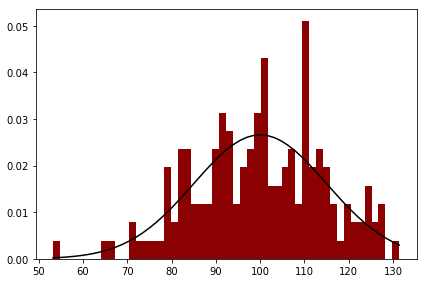
\includegraphics[width=2.0cm]{bilder/qc_reports_icon_5.png}};
			\path (p4.south)+(0.0,-1.5) \blockitem{6}{\hyperref[step5txt]{\color{green}..}5.\phantomsection\label{step5} Connected components};
			\path (p4.east)+(+7.0,0) node (ur2)[ur] {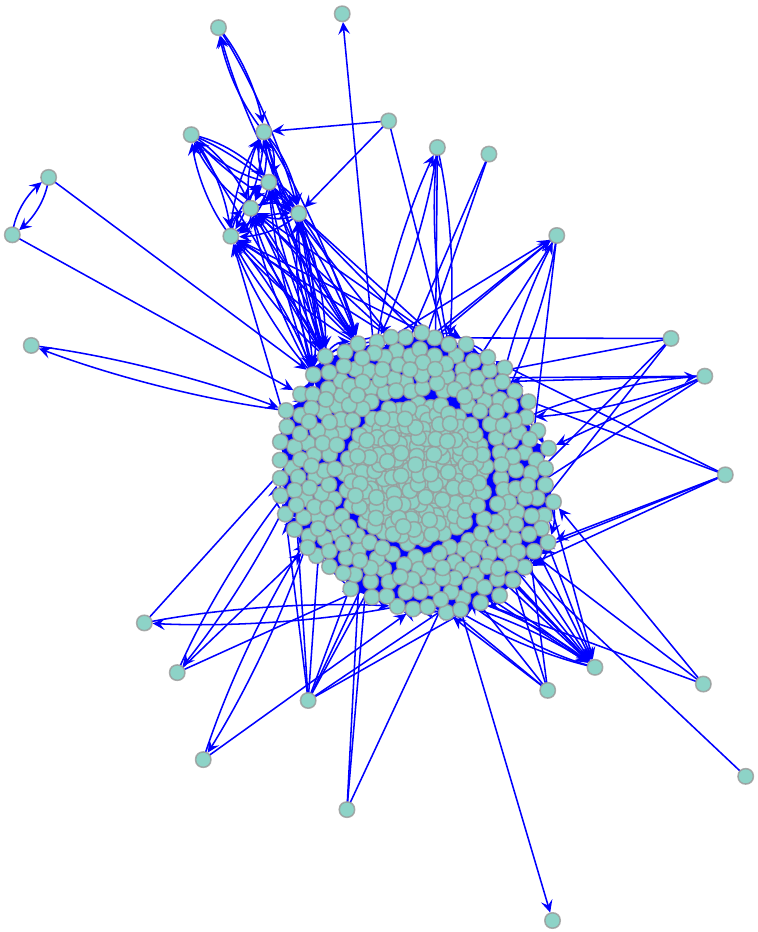
\includegraphics[width=2.0cm]{bilder/big_components_3.png}};
			\path (p6.south)+(-5.5,-1.4) \blockitem{7}{\hyperref[step7txt]{\color{green} ..}7.\phantomsection\label{step7} Allele \\combinations};
			\path (p6.south)+(0.0,-1.4) \blockitem{8}{\hyperref[step6txt]{\color{green}..}6.\phantomsection\label{step6} Candidate \\alleles};
			\path (p6.east)+(+6.5,0) node (ur3)[ur] {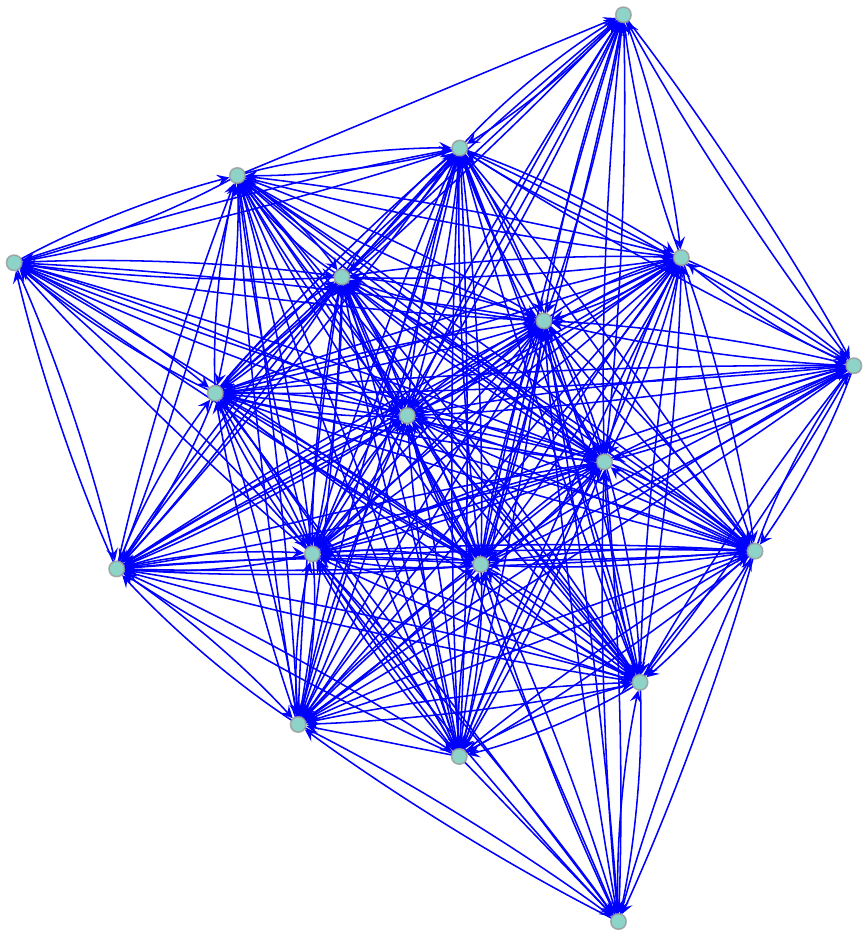
\includegraphics[width=1.0cm]{bilder/small_components_2.png}};				
			\path (p7.south)+(0.0,-3.9) \blockitem{9}{\hyperref[step8txt]{\color{green}..}8.\phantomsection\label{step8} Allele fractions};
			\path (p8.south)+(0.0,-1.5)	\blockitem{10}{\hyperref[step9txt]{\color{green}..}9.\phantomsection\label{step9} Likelihood of alleles given one read};
			\path (p9.south)+(0.0,-7.64) \blockitem{11}{\hyperref[step14txt]{\color{green}.\color{black}1}4.\phantomsection\label{step14} Indicator constrait};
			\path (p10.south)+(0.0,-1.5) \blockitem{12}{\hyperref[step10txt]{\color{green}.\color{black}1}0.\phantomsection\label{step10} Likelihood of allele fractions given one read};
			\path (p11.south)+(0.0,-1.5) \blockitem{13}{\hyperref[step13txt]{\color{green}.\color{black}1}3.\phantomsection\label{step13} Loci \\combinations};
			\path (p12.south)+(0.0,-1.5) \blockitem{14}{\hyperref[step11txt]{\color{green}.\color{black}1}1.\phantomsection\label{step11} Likelihood of allele fractions given all reads};
			\path (p14.south)+(0.0,-1.5) \blockitem{15}{\hyperref[step12txt]{\color{green}.\color{black}1}2.\phantomsection\label{step12} Maximum likelihood allele fractions};
			\path (p15.south)+(0.0,-2.0) \blockitem{16}{\hyperref[step15txt]{\color{green}.\color{black}1}5.\phantomsection\label{step15} Likelihood \\of an allele given another allele};
			\path (p16.south)+(0.0,-1.8) \blockitem{17}{\hyperref[step16txt]{\color{lime}.\color{black}1}6.\phantomsection\label{step16} Likelihood of loci given alleles and fractions}; 
			\path (p17.south)+(0.0,-1.3) \blockitem{18}{\hyperref[step17txt]{\color{green}.\color{black}1}7.\phantomsection\label{step17} Maximum likelihood loci};
			\path (p18.south)+(0.0,-1.7) \ioitem{19}{\hyperref[step18txt]{\color{green}.\color{black}1}8.\phantomsection\label{step18} VCF \\ 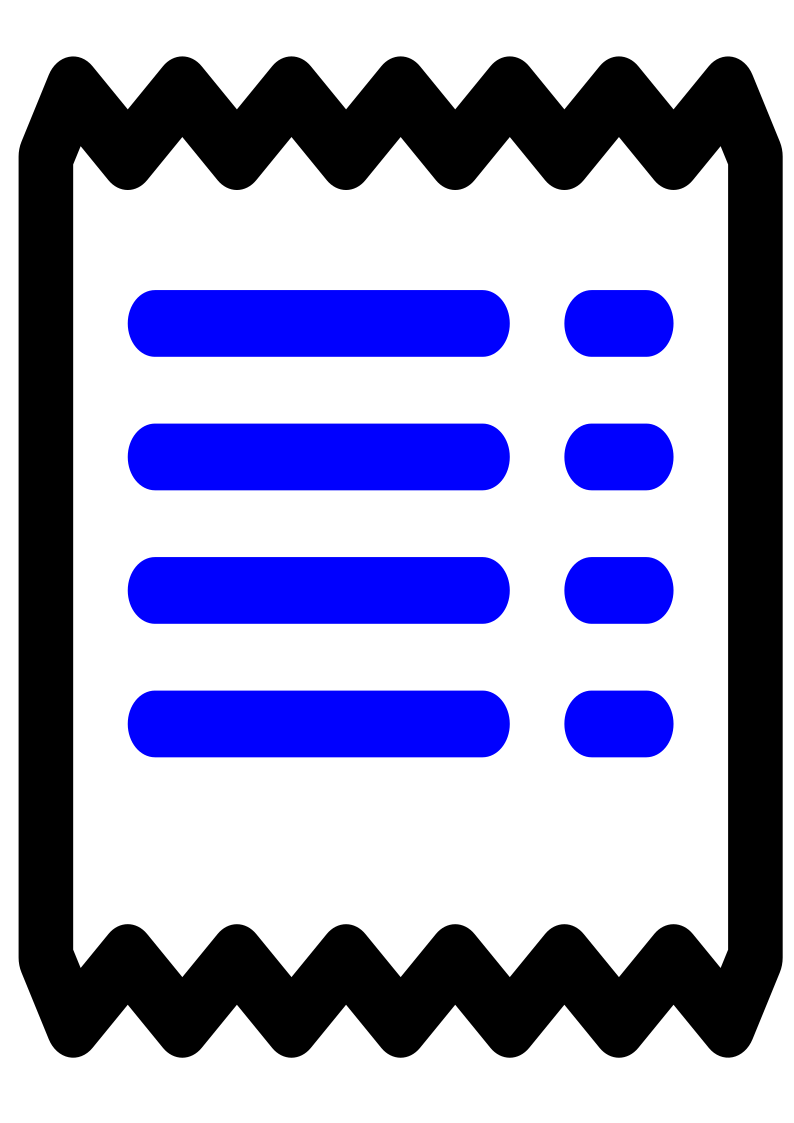
\includegraphics[width=0.9cm]{bilder/list_icon_2.png}\hspace{0.1cm}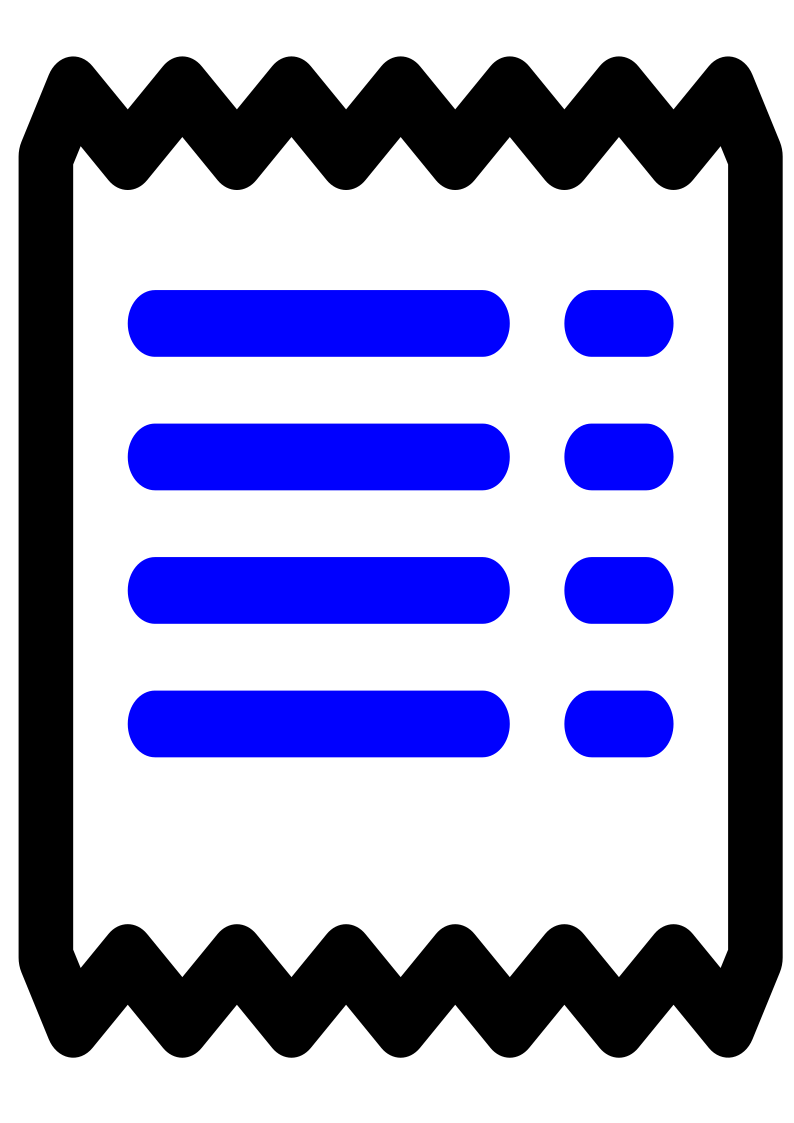
\includegraphics[width=0.9cm]{bilder/list_icon_2.png}\hspace{0.1cm}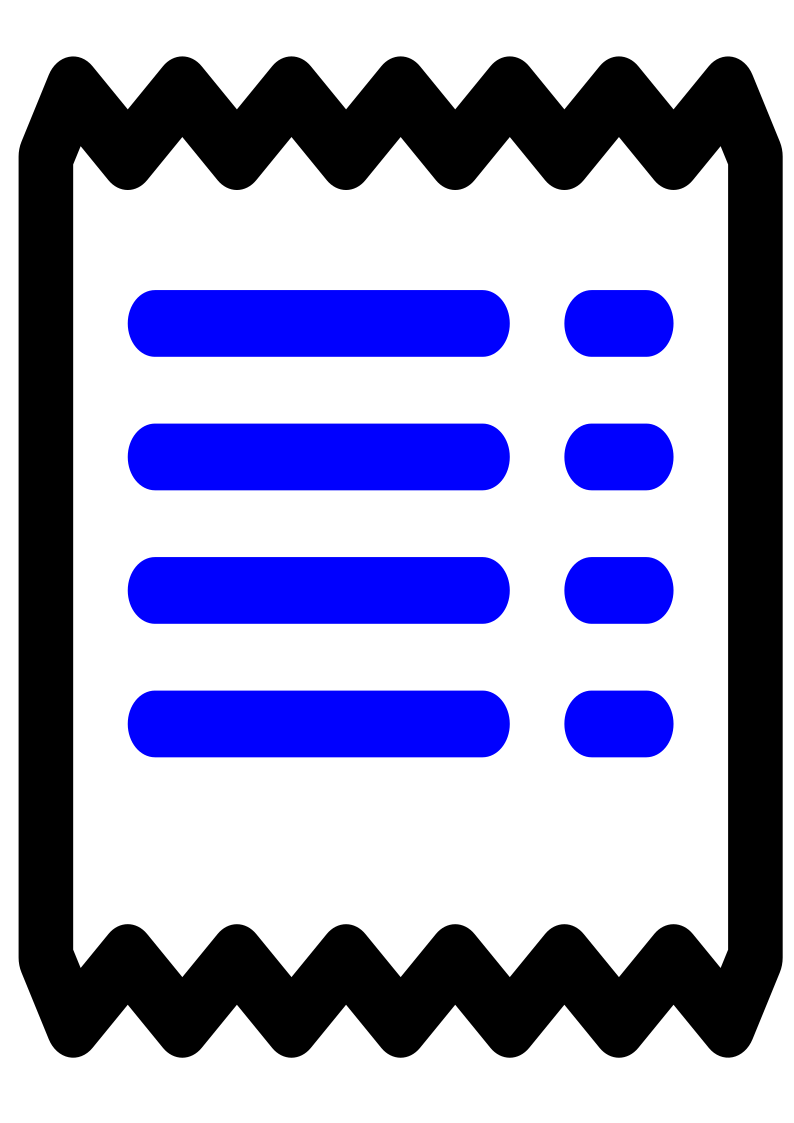
\includegraphics[width=0.9cm]{bilder/list_icon_2.png}};
			
			% Pfeile
			\path [line] (p1.south) -- +(0.0,-0.5) -- +(-2.5,-0.5) -- node [above, midway] {} (p2);
			\path [line] (p1.south) -- +(0.0,-0.5) -- +(+2.83,-0.5) -- node [above, midway] {} (p4);
			\path [line] (p2.south) -- node [above] {} (p3) ;
			\path [line] (p3.south) -- node [above] {} (p5) ;		
			\path [line] (p5.south) -- +(0.0,-1.415) -- node [above, midway] {} (p4.west);		
			\path [line] (p4.south) --node [above] {} (p6);
			\path [line] (p6.south) -- node [above] {} (p8);
			\path [line] (p8.south) -- node [above] {} (p10) ;	
			\path [line] (p10.south) -- node [above] {} (p12) ;	
			\path [line] (p12.south) -- node [above] {} (p14) ;		
			\path [line] (p14.south) -- node [above, midway] {} (p15);
			\path [line] (p15.south) -- node [above] {} (p16) ;     
			\path [line] (p16.south) -- node [above] {} (p17) ;
			\path [line] (p17.south) -- node [above] {} (p18) ;
			\path [line] (p18.south) -- node [above] {} (p19) ;		
			\path [line] (p19.south) -- +(0.0,-0.5) -- +(-8.8,-0.5) -- +(-8.8,27.498) -- node [above] {} (p5.west) ;
			
			\out{p3}{Reports (MultiQC, FastQC)}{ur1}
			\out{p4}{Graph, XML, DOT}{ur2}
			\out{p6}{Subgraphes, XML, DOT}{ur3}
			
			\path [dashedline] (p8.west) -- node [left] {} (p7);
			\path [dashedline] (p7.south) -- node [above] {} (p9) ;
			\path [dashedline] (p9.east) -- node [left] {} (p12.west);
			\path [dashedline] (p9.south) -- node [left] {} (p11.north);
			\path [dashedline] (p11.east) -- node [left] {} (p16.west);
			\path [dashedline] (p13.north) -- node [left] {} (p11.south); 
			
			\background{p3}{p2}{p3}{p5}{Preprocessing}
			\background{p3}{p4}{p4}{p6}{Graph \\construction}
			\background{p3}{p8}{p4}{p15}{Allele Likelihood}
			\background{p3}{p16}{p4}{p18}{Loci Likelihood}
 		\end{tikzpicture}
		\caption{Übersicht der Prozesse des Workflows}
		\label{fig:workflow_all}
	\end{center}
\end{figure}

\subsection{Graph und Zusammenhangskomponenten} \label{subsec:sol_graph}

Im Preprocessing erfolgt die Zuordnung der Reads zu den einzelnen Individuen und die Entfernung der Barcodes aus den Sequenzen (\hyperref[step1]{Schritt 1\phantomsection\label{step1txt}} des Workflows). Anschließend wird in \hyperref[step3]{Schritt 3\phantomsection\label{step3txt}} aus den Reads ein paarweises Sequenzalignment mit Hilfe des Tools Minimap2 ~\cite{li_2018} erzeugt. Hierbei werden alle Reads mit einander verglichen und bei ausreichender Ähnlichkeit ihrer Sequenzen einander zugeordnet. Zusätzlich werden durch Minimap2 die Edit-Distanzen zwischen den jeweils verglichenen Readsequenzen bestimmt. \\

Wie bereits einleitend erwähnt, wird das Problem schließlich als gerichteter Graph $G=(V, \, E)$ mit der Knotenmenge $V$ und der Kantenmenge $E$ betrachtet (\hyperref[step4]{Schritt 4\phantomsection\label{step4txt}} des Workflows). Die Knoten repräsentieren dabei die einzelnen Reads. Entsprechend dem von Minimap2 erzeugtem Sequenzalignment werden die Knoten der Reads durch Kanten verbunden. Die Kanten des Graphen repräsentieren somit den Vergleich der Sequenzen der beiden angrenzenden Reads. Die Anzahl der Kanten kann zusätzlich durch die von Minimap2 bestimmten Edit-Distanzen reguliert werden. Diese soll über einen konfigurierbaren Schwellwert flexibel wählbar sein und ermöglicht ein zusätzliches Filtern der Kanten zugunsten von  Laufzeit und Effizienz. \\

Da aufgrund des Sequenzalignments nur Reads mit einander verbunden werden, deren Sequenzen eine gewisse Ähnlichkeit zu einander aufweisen und da die RAD-Sequencing-Daten für gewöhnlich mehrere Loci beinhalten, ist der Graph in der Regel nicht zusammenhängend. Dies ermöglicht eine Unterteilung des Gesamtproblems in kleinere Teilprobleme durch Betrachtung der einzelnen Zusammenhangskomponenten des Graphen (\hyperref[step5]{Schritt 5\phantomsection\label{step5txt}}). Für diese Teilprobleme wird dann nach Lösungen gesucht. Da sich die Konstellation der Zusammenhangskomponenten direkt aus dem Sequenzalignment ergibt, sind die so entstandenen Cluster nicht notwendiger Weise nur einem einzigen Locus zuzuordnen. Vielmehr können die einzelnen Zusammenhangskomponenten auch jeweils mehrere Loci beinhalten. \\

\subsection{Approximation von PairHMM mittels Minimap2-Alignments} \label{subsec:phmm_minimap}

Minimap2 führt einen paarweisen Readvergleich anhand der DNA-Sequenzen der Reads durch. Die Sequenz jedes Reads (Querysequenz) wird mit jeder Sequenz der übrigen Reads (Referenzsequenz) verglichen. Reads mit hoher Ähnlichkeit zueinander werden in das Alignment aufgenommen. Das Ergebnis ist ein Mapping derjenigen Reads, die eine hohe Wahrscheinlichkeit besitzen, durch Sequenzierfehler, Variationen oder Mutationen aus einem gemeinsamen Allel hervorgegangen zu sein. Somit basieren die Kanten des Graphen auf den Wahrscheinlichkeiten des Sequenzalignments. \\

Das eigentlich zugrundeliegende Modell des Clusterings der Reads ist allerdings ein vollständiger gerichteter Graph dessen Kantengewichte durch den paarweisen Sequenzvergleich über ein pair Hidden Markov Model (pairHMM)~\cite{durbin_1998} errechnet werden. Das beobachtete Ergebnis der Referenzsequenz wird dabei durch Abfolgen von Mismatch-, Insertions und Deletions-Operationen der Querysequenz erklärt (Evaluationsproblem). Jede dieser Operationen stellt einen Zustand dar, der Übergang zwischen den Zuständen wird über Wahrscheinlichkeiten abgebildet. Die Zustände selbst sind allerdings nicht direkt beobachtbar. Die möglichen Kombinationen von Zustandsübergängen, die zum beobachteten Ergebnis der Referenzsequenz führen, können aber errechnet und als Matrix dargestellt werden. In der Matrix kann dann der wahrscheinlichste Pfad ermittelt werden. Als Ergebnis erhält man somit die Zustandssequenz mit maximaler Likelihood, um die Querysequenz in die Referezsequenz zu transformieren, dieser entspricht der Kantengewichtung des Graphen. Die Kantengewichte können schließlich anhand eines Schwellenwertes gefiltert werden, so nur Kanten mit ausreichender Likelihood zurückbleiben. Je nach gewähltem Schwellwert wird der Graph hierdurch in mehrere Zusammenhangskomponenten partitioniert und das Problem kann über die entstandenen Teilprobleme gelöst werden. \\

Die Bestimmung der Kantenwahrscheinlichkeiten mittels pairHMM ist sehr rechenintensiv und wirkt sich entsprechend ungünstig auf die Laufzeit aus~\cite{durbin_1998, yoon_2009}. Stattdessen kann das durch Minimap2 generierte Sequenzalignmment für diploide Organismen als Approximation des pairHMM verwendet werden, polyploide Organismen benötigen stattdessen für die Locizuordnung ein multiples Sequenzalignment (siehe Kap. \ref{sec:ausblick}). Jedes Alignment aus Minimap2 repräsentiert bereits den wahrscheinlichsten Pfad einer pairHMM-Matrix. Daher genügt es die Likelihood $ L_{i} $ über diesem Alignment hinsichtlich des Sequenzierfehlerrate bei der Auswahl der Allele (siehe Kap. \ref{subsec:sol_allele_lh}) bzw. hinsichtlich der Heterozygotiewahrscheinlichkeiten bei der Zuordnung der Loci (siehe Kap. \ref{subsec:sol_loci_lh}) zu berechnen. Diese Likelihoodberechnungen sollen zur besseren Sicht auf das Modell bereits an dieser Stelle besprochen werden, auch wenn dadurch einige Schritte des Workflows vorweg genommen werden.

\subsubsection{Likelihoodberechnung der Allele bei einem gegebenen Read} \label{pHMM_alleles}

Um die Wahrscheinlichkeit zu bestimmen, dass ein Read mit der Readsequenz $s_{r}$ und der Fehlerrate $\epsilon$ tatsächlich aus einem bestimmten Allel hervorgegangen (\hyperref[step9]{Schritt 9\phantomsection\label{step9txt}} des Workflows), muss die Sequenzierfehlerrate berücksichtigt werden. Die Zustandssequenz des approximierten pairHMM lässt sich dem CIGAR-String des Minimap2-Alignments entnehmen. Für jede Base der Querysequenz wird entsprechend den Operationen des CIGAR-Strings wird Sequenzierfehlerwahrscheinlichkeit auf unterschiedliche Weise in die Likelihoodberechnung einbezogen. \\

Bei einem Match sind beide Basen aus Query- und Referenzsequenz identisch. Daher ergibt sich die Wahrscheinlichkeit $L_{match}$, dass es sich bei Querysequenz an Position $i$ tatsächlich um die korrekte Base handelt allein aus der Fehlerrate. Die geschätzte Fehlerrate $ p_{i} $ lässt sich anhand der Basenqualität des Reads nach \eqref{eqn:3-3} bestimmen (vgl. Kap. \ref{subsec:lh_allele}). Die resultierende Likelihood der Base wird um diese Fehlerrate reduziert:
\vspace{-0.5cm}
\begin{center}
	\fcolorbox{black}{white}{		
		\parbox{\textwidth}{
			\begin{equation} \label{eqn:2-13}
			\tag{2-13}
			L_{match} = 1 - p_{i}
			\end{equation}
        }}
\end{center}
Für Insertionen und Deletionen werden empirisch ermittelte Sequenzierfehlerraten $\epsilon_{ins}$ und $\epsilon_{del}$ verwendet \cite{schirmer_2016}: 
\vspace{-0.5cm}
\begin{center}
	\fcolorbox{black}{white}{		
		\parbox{\textwidth}{
			\begin{equation} \label{eqn:2-22}
			\tag{2-22}
			L_{indel} \in \{\epsilon_{ins}, \epsilon_{del}\}
			\end{equation}
        }}
\end{center}

Bei Substitutionen ergibt sich die Sequenzierfehlerrate ebenfalls aus der geschätzten Fehlerrate $p_{i}$ im Bezug auf die Basenqualität des Queryreads $q_{query}$. Die Likelihood $L_{sub}$, dass anstelle der sequenzierten Base tatsächlich eine der drei anderen Basen vorliegt, entspricht dabei $ 1/3 $ der geschätzten Fehlerrate~\cite{kuhner_2014}.
\vspace{-0.5cm}
\begin{center}
	\fcolorbox{black}{white}{		
		\parbox{\textwidth}{
			\begin{equation} \label{eqn:2-8}
			\tag{2-8}
			L_{sub} = \frac{1}{3} \; \cdotp \; p_{i}
			\end{equation}
        }}
\end{center}

Die Likelihood $ pairHMM_{\epsilon, q_{query}} \;(s_{ref}\;|\; s_{query}) $, dass der Queryread aus dem Referenzread allein durch Sequenzierfehler entstanden ist, errechnet sich schließlich aus dem Produkt der Likelihoods $ L_{i} \in \{L_{match}, L_{indel}, L_{sub}\} $ für jede Position $ i $ der Sequenz des Queryreads $ s_{query} $ im Vergleich zum Referenzread $ s_{ref} $.
\vspace{-0.5cm}
\begin{center}
	\fcolorbox{black}{light-gray}{		
		\parbox{\textwidth}{
			\begin{equation} \label{eqn:2-5}
			\tag{2-5}
			pairHMM_{\epsilon, q_{query}} \;(s_{query}\;|\; s_{ref}) = \prod_{i=1}^{k}L_{i}
			\end{equation}
        }}
\end{center}
 
Durch die Berücksichtigung der Basenqualität fließen Sequenzierfehler mit geringerer Likelihood in die weitere Berechnung ein. Dadurch wird auch die Likelihood bei der späteren Locizuordnung für Reads mit Sequenzierfehlern geringer ausfallen. Insgesamt werden an dieser Stelle also die Sequenzierfehler herausgefiltert, da es auf diese Weise nicht möglich ist eine bessere Likelihood unter Einschluss eines Reads mit Sequenzierfehlern bei der Locizuordnung zu erreichen, als ohne diesen Read (siehe Kap. \ref{subsec:sol_loci_lh}).

\subsubsection{Likelihoodberechnung bei der Zuordnung der Allele zu möglichen Loci} \label{pHMM_loci}

Ein weiteres Mal wird auf die Approximation des pairHMM durch Minimap2 zurückgegriffen, um die Menge der wahrscheinlichsten Allele einer Zusammenhangskomponente sinnvollen Locikombinationen zuordnen zu können (\hyperref[step15]{Schritt 15\phantomsection\label{step15txt}} des Workflows). Hierfür können bei diploiden Spezies die Allele ebenfalls paarweise unter Berücksichtigung der Hetereozygotiewahrscheinlichkeiten $\eta_{sub}$, $\eta_{ins}$ und $\eta_{del}$ mit einander verglichen werden. Auch hier wird die Sequenz eines der Allel (Query) gegen die Sequenz ein anderes Allels (Referenz) verglichen. Entsprechend den Operationen des CIGAR-Strings wird die Likelihood für jede Position $i$ der Querysequenz bestimmt. \\

Im Falle eines Matches senken sämtliche Heterozygotiewahrscheinlichkeiten die Likelihood $L_{match}$, dass beide Allele vom gleichen Locus stammen (Formel \eqref{eqn:2-11}).
\vspace{-0.5cm}
\begin{center}
	\fcolorbox{black}{white}{		
		\parbox{\textwidth}{
			\begin{equation} \label{eqn:2-11}
			\tag{2-11}
			L_{match} = 1 - (\eta_{sub} + \eta_{ins} + \eta_{del})
			\end{equation}
        }}
\end{center}
Bei einem Mismatch entspricht die Likelihood $L_{mismatch}$ der Heterozygotiewahrscheinlichkeit $ \eta $ der betreffenden Mutationsart, also $ \eta_{sub} $ für Substitutionen , $ \eta_{ins} $ für Insertionen bzw. $ \eta_{del} $ bei Deletionen. 
\vspace{-0.5cm}
\begin{center}
	\fcolorbox{black}{white}{		
		\parbox{\textwidth}{
			\begin{equation} \label{eqn:2-10}
			\tag{2-10}
			L_{mismatch} \in  \{\,\eta_{sub},\, \eta_{ins},\, \eta_{del}\,\}
			\end{equation}
        }}
\end{center}

Die Wahrscheinlichkeit $ pairHMM_{\eta}(a_{l_{j,query}} \, | \, a_{l_{j,ref}}) $ des  paarweisen Vergleichs zweier Allele hinsichtlich eines Locus $l_{j}$ errechnet sich wieder aus dem Produkt der Wahrscheinlichkeiten $L_{i} \in \{L_{match}, \, L_{mismatch}\}$ der einzelnen Basen:
\vspace{-0.5cm}
\begin{center}
	\fcolorbox{black}{light-gray}{		
		\parbox{\textwidth}{
			\begin{equation} \label{eqn:2-14}
			\tag{2-14}
			pairHMM_{\eta}(a_{l_{j,query}} \, | \, a_{l_{j,ref}}) = \prod_{i=1}^{k}L_{i}
			\end{equation}
        }}
\end{center}

Daraus ergibt sich nach Formel \eqref{eqn:2-12} die Likelihood $ Pr(T=a_{l_{j,2}} \, | \, S=a_{l_{j,1}}, \eta) $, dass zwei Allele $a_{l_{j,1}}$ und $a_{l_{j,2}}$ vom gleichen Locus $l_{j}$ stammen.
\vspace{-0.5cm}
\begin{center}
	\fcolorbox{black}{light-gray}{		
		\parbox{\textwidth}{
			\begin{equation} \label{eqn:2-12}
			\tag{2-12}
			Pr(T=a_{l_{j,2}} \, | \, S=a_{l_{j,1}}, \eta) = pairHMM_{\eta}(a_{l_{j,1}}, a_{l_{j,2}})
			\end{equation}
        }}
\end{center}

\subsection{Allele-Fractions mit maximaler Likelihood} \label{subsec:sol_allele_lh}
\subsubsection{Bestimmung der Kandidatenallele und der Allele-Fractions} \label{outsubsec:sol_cand_allele}

Um später die Allele zu identifizieren, von denen die beobachteten Reads einer Zusammenhangskomponente am wahrscheinlichsten stammen, muss zunächst die Menge der Kandidatenallele $A=(a_{1}, \dots, a_{n}) \in \{A,\,C,\,G,\,T,\}^{k^n}$ bestimmt werden (\hyperref[step6]{Schritt 6\phantomsection\label{step6txt}} des Workflows). Bei größeren Clustern ist davon auszugehen, dass die Sequenzen solcher Kandidatenallele mehrfach in den Reads auftauchen. Um den Aufwand der Likelihoodberechnung bei größeren Cluster anpassen zu können, soll es möglich sein, selten auftretende Sequenzen herauszufiltern. Dies geschieht über Grenzwerte, welche die Mindestgröße der Cluster und die Mindesthäufigkeiten von Kandidatenallelsequenzen berücksichtigen sollen. \\

Über der Menge der Kandidatenallele sollen nun mögliche Allelkombinationen erzeugt werden (\hyperref[step7]{Schritt 7\phantomsection\label{step7txt}}), die später den Loci zugeordnet werden. Die Länge dieser Kombinationen, also die erwartbare Anzahl von Allelen $n_{alleles}$, die auf einen oder mehrere Loci verteilt sind, ergibt sich dabei aus der Anzahl der Kandidatenallele $n_{cand}$ und der Ploidie $\phi$. Sie entspricht also entweder direkt der Ploidie, falls diese höher ist als die Anzahl der Kandidatenallele oder andernfalls gilt $n_{alleles} \geq n_{cand}$, so dass $n_{alleles}$ ein ganzzahliges Vielfaches der Ploidie ist. Dies ist in Formel \eqref{eqn:2-1} formal dargestellt, wobei gilt $d=n_{cand} \mod \phi$.

\begin{equation} \label{eqn:2-1}
\tag{2-1}
n_{alleles} =
\left\{
\begin{array}{ll}
\phi, & \phi \geq n_{cand} \\
n_{cand} + \phi - d, & \phi < n_{cand} \wedge d \neq 0\\
n_{cand}, & \phi < n_{cand} \wedge d = 0
\end{array}
\right.
\end{equation}

Die Zusammenhangskomponenten können auch mehrere Loci enthalten, so dass in ihnen die einzelnen Allele mehrfach in verschiedenen Loci oder homozygot innerhalb eines Locus vorkommen können. Hinsichtlich der Allelkombinationen müssen also Wiederholungen der Allele erlaubt sein. Nach dem Urnenmodell werden dabei $n_{alleles}$ Allele mit Zurücklegen aus insgesamt $ n_{cand} $ verschiedenen Allelen kombiniert, wobei die Reihenfolge keine Relevanz hat. Dies wird in Kap. \ref{sec:max_lh_allele} ausführlicher dargelegt. \\

Für jede Allelkombination werden anschließend die relativen Häufigkeiten der darin enthaltenen Allele bestimmt (\hyperref[step8]{Schritt 8\phantomsection\label{step8txt}} des Workflows). Diese repräsentieren die Häufigkeitsverteilung der Allele der jeweiligen Kombination und werden im Folgenden als Allele-Fractions oder VAFs bezeichnet.\\

\subsubsection{Bestimmung der Likelihood eines Alleles im Bezug auf einen Read} \label{sol_al_read}

Für jeden Read wird nun in \hyperref[step9]{Schritt 9} des Workflows die Wahrscheinlichkeit bestimmt, dass er aus einem bestimmten Allel allein durch Sequenzierfehler hervorgegangen ist. Dies genaue Berechnung der Likelihood wurde in Kap. \ref{pHMM_alleles} bereits vorgestellt. \\

In Zusammenschau mit Formel \eqref{eqn:2-5} lässt sich beim paarweisen Vergleich eines Read mit der Sequenz $s_{r}$ und dem Kandidatenallel $a_{i} \in A $ die Likelihood $ Pr(T=s_{r} \, | \, S=a_{i}, \epsilon) $ unter Berücksichtigung der Fehlerrate $\epsilon$ wie folgt errechnen:
\vspace{-0.5cm}
\begin{center}
	\fcolorbox{black}{light-gray}{		
		\parbox{\textwidth}{
			\begin{korollar*}[Likelihood eines Kandidatenallels gegeben ein Read]
				\begin{equation} \label{eqn:2-15}
				\tag{2-15}
				Pr(T=s_{r} \, | \, S=a_{i}, \epsilon) = pairHMM_{\epsilon,q_{r}}(a_{i}, s_{r})
				\end{equation}
			\end{korollar*}
		}}
\end{center}

\subsubsection{Bestimmung der Likelihood einer Allele-Fraction im Bezug auf einen Read} \label{sol_vaf_one_reads}

In \hyperref[step10]{Schritt 10\phantomsection\label{step10txt}} des Workflows wird anschließend die Wahrscheinlichkeit ermittelt, einen bestimmten Read $s_{r}$ anhand einer gegebenen Allele-Fraction $\Theta_{i} = (\theta_{1},\dots,\theta_{n_{cand}}) \in [0,1]^n_{cand}$ zu beobachten. Hierzu wird die in Formel \eqref{eqn:2-15} ermittelte Likelihood auf die relativen Häufigkeiten aller Kandidatenallele $ (\theta_{1},\dots,\theta_{n}) $ der Allele-Fraction bezogen.\\

Da eine Zusammenhangskomponente auch mehrere Loci enthalten kann, sollen nun die Fractions in einer möglichen Menge von Loci ermittelt werden. Nach dem oben genannten Urnenmodell entspricht dies der Wahrscheinlichkeit, dass bei Auswahl von $n_{alleles}$ Elementen (siehe Kap. \ref{subsec:sol_allele_lh}) das Kandidatenallel $ a_{i}$ mit einer Häufigkeit von genau $\theta_{i}$ vorliegt. Es wird also die Multinomialverteilung der Kandidatenallele betrachtet. Dabei muss sich die Wahrscheinlichkeit aus den tatsächlichen Beobachtungen ergeben, so dass die Likelihood $Pr(s_{r} \, | \, \Theta=\theta_{1},\dots,\theta_{n})$ aus der Multinomialverteilung $\theta_{i}$ im Bezug auf die individuelle Verteilung $Pr(T=s_{r} \, | \, S=a_{i}, \epsilon)$ nach Formel \eqref{eqn:2-17} bestimmt wird. Im Hinblick auf die Zuordnung zu einem oder mehreren möglichen Loci muss für jede Allele-Fraction gelten, dass $\sum \theta_{i} = 1$.
\vspace{-0.5cm}
\begin{center}
	\fcolorbox{black}{light-gray}{		
		\parbox{\textwidth}{
			\begin{korollar*}[Likelihood einer Allele-Fraction gegeben ein Read]
				\begin{equation} \label{eqn:2-17}
				\tag{2-17}
				Pr(s_{r} \, | \, \Theta=\theta_{1},\dots,\theta_{n}) = \sum_{i=1}^{n}\theta_{i} \, \cdotp Pr(T=s_{r} \, | \, S=a_{i}, \epsilon)
				\end{equation}
    		\end{korollar*}
 		}}
\end{center}
\subsubsection{Bestimmung der Likelihood einer Allele-Fraction im Bezug auf alle Reads} \label{sol_vaf_all_reads}

Schließlich soll in \hyperref[step11]{Schritt 11\phantomsection\label{step11txt}} die resultierende Likelihood einer Allele-Fraction in Zusammenschau mit allen Reads bestimmt werden. Die Unsicherheit bei der Zuordnung der Reads wird dabei durch die relativen Häufigkeiten in der Allele-Fraction abgebildet und an die spätere Loci-Zuordnung (Kap. \ref{subsec:sol_loci_lh}) weitergereicht. Sei $L \in \{l_{i} \in \mathds{N}_{\leq n}^\phi \, | \, i=1, \dots, g\}$ die Menge möglicher Loci, die durch eine Allele-Fraction abgebildet wird und $D = (s_{1}, \dots, s_{m}) \in \{A,C, G, T\}^{k^m}$ die Menge der Readsequenzen. Die Menge möglicher Loci für eine Allel-Fraction ergibt sich dabei aus Likelihood $Pr(D \, | \, \Theta)$ der Allel-Fraction $\Theta$ über alle Readsequenzen $D$. Und lässt sich als Produkt der Likelihoods $Pr(s_{r} \, | \, \Theta)$ der Allele-Fractions für jeden Read ausdrücken: 
\vspace{-0.5cm}
\begin{center}
	\fcolorbox{black}{light-gray}{		
		\parbox{\textwidth}{
 		\begin{korollar*}[Likelihood einer Allele-Fraction gegeben alle Reads]
			\begin{equation} \label{eqn:2-18}
			\tag{2-18}
			L(\Theta=\theta_{1},\dots,\theta_{n} \, | \, D) = Pr(D \, | \, \Theta=\theta_{1},\dots,\theta_{n}) = \prod_{r=1}^{m}Pr (s_{r} \, | \, \Theta=\theta_{1},\dots,\theta_{n})
			\end{equation}
		\end{korollar*}
	}}
\end{center}

Die \hyperref[step9]{Schritte 9}, \hyperref[step10]{10} und \hyperref[step11]{11} des Workflows werden für alle Allele-Fractions jeder Zusammenhangskomponente durchgeführt. Für jedes Kandidatenallel aller Allel-Fractions wird so die Wahrscheinlichkeit berechnet, dass die Reads der Zusammenhangskomponente aus den einzelnen Kandidatenallelen entstanden sind. Da nur die Fehlerrate $\epsilon$ einbezogen wurde, können alle dabei entstandenen Abweichungen ausschließlich auf Sequenzierfehlern beruhen. Um diejenige Allel-Fraction zu wählen, deren Verteilung der Kandidatenallelsequenzen am besten zusammen passen, wird in \hyperref[step12]{Schritt 12\phantomsection\label{step12txt}} aus der Menge der errechneten Likelihoods aller Allele-Fractions das Maximum bestimmt.  

\subsection{Locuszuordnung mit maximaler Likelihood} \label{subsec:sol_loci_lh}


\noindent======================= draft =======================\\



connected comp in loci aufsplitten\\
Zuordnung zu loci, also welche genomischen loci stecken dahinter, wie werden die allele den loci zugeordnet -> max parsimony, prinzip der einfachsen möglichen lösung \\
-> ploidy als eingabeparam -> zuordnung der candidaten allele zu loci\\
lh ausrechnen aus anzahl der allele und loci -> gerade die loci, die die seq. der reads am besten unter der geg. ploidy und heterozygotie erklären haben max lh
max\_lh\_vafs nur noch 1 Vektor\\
Zuordnung von cand-Allelen zu den loci => die beobachteten max\_lh\_allel\_fractionen müssen sie durch die gewählten loci erklären, z.B. 2 loci => 1.locus: allel 0, 0 homozyg, 2. locus allel 0, 2 heterozygot\\
-> bei z.B 3 Allelen sind min 2 Loci notwendig => min \# der loci, so dass alle ausgewählten allele passen -> diese menge muss gefunden werden und muss wieder max lh haben\\
unter der annahme der loci-verteilung muss bestimmt werden ob sinnvoll, d.h allel-vafs müssen sich zu 1 summieren -> indikator-funktion: wenn 1, dann gilt Pr(T|S), d.h. Wslk, dass sich aus S die seq T gebildet hat\\

indicator-function $z_{l} \in {[0,1]}$: wird 1, wenn anzahl des auftretens aller allele $A = (a_{1}, \dots, a_{n})$ in einer möglichen locus-verteilung $l = (l_{1}, \dots, l_{g \, \cdotp \phi})$ jeweils genau ihrer absoluten Häufigkeit aus der in Kap. \ref{subsec:sol_allele_lh} errechneten vaf mit maximaler Likelihood entspricht, also $\theta_{i} \, \cdotp g \, \cdotp \phi$ entsprechen, andernfalls gilt $ z_{l} = 0 $. Seien dabei  $\Theta=\theta_{1},\dots,\theta_{n}) \in [0,1]^n $ die vaf mit maximaler Likelihood, $ \phi $ die Ploidie und gilt für eine mögliche Locusverteilung $l$ außerdem $L \in \{l_{j} \in \mathds{N}_{\leq n}^\phi \, | \, j=1, \dots, g\}$, so lässt sich die Indikatorfunktion wie folgt definieren:
\begin{equation} \label{eqn:2-19}
\tag{2-19}
z_{l}=\prod_{i=1}^{n}1_{\sum_{j=1}^{g}\sum_{k=1}^{\phi}1_{l_{j,k}=i} = \theta_{i} \, \cdotp g \, \cdotp \phi}
\end{equation}

pHMM: Wslk, dass allel 2 $ a_{l_{j,2}} $ aus allel 1 $ a_{l_{j,1}} $ entstanden ist -> heterozygotie $\eta$ (in conf konfigurierbar) =>$ match = 1 - (het_{sub} + het_{del} + het_{ins}) $
\begin{equation} \label{eqn:2-20}
\tag{2-20}
Pr(T=a_{l_{j,2}} \, | \, S=a_{l_{j,1}}, \eta) = pairHMM_{\eta}(a_{l_{j,1}}, a_{l_{j,2}})
\end{equation}

Kombi von loci -> lh berechnen
\begin{equation} \label{eqn:2-21}
\tag{2-21}
Pr(\Theta,A \, | \, L=\{l_{j}\, |\, j=1,\dots,g\})=z_{l} \, \cdotp \prod_{j=1}^{g}Pr(T=a_{l_{j,2}} \, | \, S=a_{l_{j,1}})
\end{equation}

=> maximum der loci Likelihoods wählen
\subsection{Varianten und Genotyp} \label{subsec:sol_vcf}
mit den allelen $A = (a_{1}, \dots, a_{n})$ jedes locus $L \in \{l_{j} \in \mathds{N}_{\leq n}^\phi \, | \, j=1, \dots, g\}$, allelsequenz, genotyp\\
Menge von Loci, die die Beobachtungen erklären
% kapitel3.tex
\chapter{Algorithmus} \label{sec:alg}
Für das hier implementierte RAD-Sequencing-Tool, NodeRAD, wurde zur Workflowintegration das Workflow Management System Snakemake verwendet ~\cite{koester_2012_1, koester_2012_2}. Die einzelnen Analyseschritte werden dabei über Regeln abgebildet. Für jede Regel können neben dem zu verwendenden Script oder Shell-Kommando sowie den Pfadangaben für In- und Output auch zusätzliche Optionen festgelegt werden. Dazu gehören beispielsweise Angaben zu Parametern bzw. Argumenten für die verwendeten Tools, Pfadangaben für Log-Dateien oder die Anzahl der zu verwendenden Threads.

Als Input benötigt der Workflow eine Datei im FASTQ-Format, welche die single-end Reads der verschiedenen Individuen mit ihren Identifikationsbezeichnungen, der Basensequenz und Angaben zur  Basenqualität enthält. Des Weiteren wird eine Tabelle im tsv-Format benötigt, in der die Zuordnung der Probennamen zu den Individuen und ihren Barcode-Sequenzen definiert ist. Nach dem Preprocessing, der Qualitätskontrolle der Reads und dem Sequence-Alignment erfolgt die RAD-Seq-Analyse durch NodeRAD. Hierbei werden die Wahrscheinlichkeiten der Allelsequenzen und der möglichen Loci bestimmt. Die Loci mit der höchsten Wahrscheinlichkeit werden schließlich mit den Sequenzen ihrer Allele und den möglichen Varianten entsprechend dem ermittelten Genotyp in einer Datei im Variant Call Format (VCF) ausgegeben.

\section{Preprocessing} \label{sec:preproc}

Im Preprocessing werden durch das Tool Cutadapt ~\cite{martin_2011} die Reads jedes Individuums anhand ihrer Barcodesequenzen identifiziert und extrahiert (Demultiplexing). Hiernach werden die Barcodesequenzen entfernt (Trimming) und die Reads jedes Individuums in separaten Dateien im FASTQ Format abgelegt. \\
Im Anschluss an das Trimming erfolgt eine Qualitätskontrolle durch das Tool FastQC  ~\cite{andrews_2012}. Dabei werden einige allgemeine Statistiken zu den Rohdaten der Reads generiert, wie beispielsweise zur Basenqualität, zum GC-Gehalt, dem Anteil an Duplikaten oder überrepräsentierten Sequenzen. Durch das Tool MultiQC ~\cite{ewels_2016} wird aus diesen Statistiken und den Log-Dateien von Cutadapt ein html-Report mit diversen Plots zur Veranschaulichung erstellt.

\section{Edit-Distanzen} \label{sec:edit}
Für die spätere Konstruktion eines Graphen basierend auf den Edit-Distanzen zwischen den Readsequenzen wird für jedes Individuum zunächst ein Sequenzalignment mit Hilfe des Tools Minimap2 ~\cite{li_2018} erstellt. Hierbei werden alle Readsquenzen paarweise verglichen und in Abhängigkeit von ihren Übereinstimmungen (Matches) und Unterschieden (Mismatches) einander zugeordnet. Das Ergebnis des Mappings wird im sam-Format ~\cite{li_2009} ausgegeben und enthält Angaben zur betrachteten Sequenz (Query), die gegen einen anderen Read (Reference) verglichen wurde. Neben den ID's der Query- und Reference-Sequenzen, werden dort unter anderem auch der CIGAR-String, Informationen zur Basenqualität der Query-Sequenz, sowie optional verschiedene Tags angegeben. Ein für die späteren Berechnungen wichtiges Maß sind die Edit-Distanzen, die durch den NM-Tag repräsentiert werden. Die Edit-Distanz gibt hierbei die minimale Anzahl von Editieroperationen an, um die Query-Sequenz in die Referenzsequenz zu transformieren. Als Editieroperationen sind hierbei ersetzen, einfügen und löschen von Basen möglich. Auf DNA-Ebene entspricht dies den Punktmutationen im Sinne von Substitutionen, Insertionen und Deletionen (vgl. Kap. \ref{subsec:mutation}). Der CIGAR-String ist eine kondensierte Darstellung der Unterschiede zwischen Query- und Reference-Sequenz. In ihm werden Matches und Mismatches wie Insertionen, Substitutionen und Deletion jeweils mit der Anzahl der betroffenen Basen angegeben. Sowohl der CIGAR-String als auch der NM-Tag definieren wichtige Kanteneigenschaften des späteren Graphen. \\

\section{Konstruktion des Graphen} \label{sec:graph}
\subsection{Knoten des Graphen} \label{subsec:nodes}
Das hier in Python implementierte Tool, NodeRAD, benötigt als Input zu jedem Individuum die getrimmten single-end Read-Daten sowie das Sequenzalignment. Zunächst wird daraus für jedes Individuum ein eigener, gerichteter Graph $ G $ mit $ G = (V,E) $ erstellt. Seine Knoten, $ V $, werden durch die einzelnen Reads repräsentiert. Entsprechend ergeben sich die Knoteneigenschaften aus den Daten der Reads, diese werden den FASTQ-Dateien nach Ausführung von Cutadapt (siehe \ref{sec:preproc}) entnommen. Die Kanten, $ E $, zwischen den Knoten ergeben sich aus dem Vergleich ihrer Sequenzen im Rahmen des Sequenzalignments mittels Minimap2 (siehe \ref{sec:edit}).\\

Zusätzlich entnimmt NodeRAD der Konfigurationsdatei des Workflows einige Konstanten und Grenzwerte für die späteren Berechnungen. Dazu gehören die Mutationsraten und Heterozygotiewahrscheinlichkeiten für Substitutionen, Insertionen und Deletionen, die Ploidie des Chromosomensatzes der untersuchten Spezies und Grenzwerte. Die Konstanten werden als Grapheigenschaften im Graphen abgelegt. Als konfigurierbare Grenzwerte gibt es für NodeRAD einen Schwellenwert für die maximal zulässige Editierdistanz, bei dem zwei Knoten noch durch eine Kante verbunden werden sowie Schwellenwerte zum Filtern selten vorkommender Sequenzen ab einer bestimmten Clustergröße, die als Hintergrundrauschen nicht in der Berechnung Berücksichtigung finden sollen. \\

Zur Konstruktion des Graphen wird die Python-Library graph-tool ~\cite{peixoto_2014} genutzt. Die Knoten werden aus den FASTQ-Daten der getrimmten Reads mittels SeqIO aus der Library Biopython ~\cite{cock_2009_1} ausgelesen und im Graphen mit den Knoteneigenschaften ihrer Basensequenz, einer internen ID sowie Angaben zur Basenqualität abgelegt. Die Codierung des Qualitystrings der Reads variiert je nach verwendeter Platform. Daher wird er durch SeqIO ausgelesen und für jede Base in ein einheitliches Maß, den Phred Quality Score $ Q $, decodiert ~\cite{cock_2009_2}. Zusätzlich wird aus den Phred Quality Scores die geschätzte Fehlerwahrscheinlichkeit $ P $ für jede Base nach Formel \eqref{eqn:3-1} bestimmt ~\cite{ewing_1998}.  

\begin{equation} \label{eqn:3-1}
    \tag{3-1}
    P = 10^{\frac{-Q}{10}}
\end{equation}

Für jeden Knoten werden die Vektoren mit den Phred Qualitiy Scores und den geschätzen Fehlerwahrscheinlichkeiten der Basen des Reads als Knoteneigenschaften gespeichert. \\

Die Laufzeit für das Hinzufügen eines Knotens beträgt nach der Dokumentation von graph-tool  $ O(V) $, da es sich hierbei um eine Einfügeoperation in die bereits bestehende Knotenmenge handelt und ein neuer Iterator über alle Knoten erzeugt und zurückgegeben wird ~\cite{docs_graph_tool}. Die Zuweisung der Knoteneigenschaften erfolgt in $ O(1) $. Über alle Reads, also über die resultierende Anzahl der Knoten $ V $ ergibt sich daraus eine Gesamtlaufzeit von $ O(V^2) $.\\

\subsection{Kanten des Graphen} \label{subsec:edges}
Die Kanten des Graphen definieren sich durch das mittels Minimap2 erzeugten Sequenzalignments (vgl. Kap. \ref{sec:edit}). Jedes Alignment zwischen zwei Reads entspricht im Graphen einer gerichteten Kante $e = (source,\; target)$, die den Vergleich der Query- zur Referenzsequenz repräsentiert. Sie verbindet somit zwei der zuvor aus der FASTQ-Daten erzeugten Knoten. Das Auslesen des sam-Formats des Alignmentfiles erfolgt mit Hilfe der Python-Library pysam ~\cite{pysam}. Dabei wird die Edit-Distanz aus dem NM-Tag zunächst genutzt, um nur Kanten in den Graphen aufzunehmen, die bereits einen optimierten Minimap2-Path darstellen. Liegen diese unterhalb des durch die Konfigurationsdatei festgelegten Grenzwertes, so wird die Kante dem Graphen hinzugefügt. Dabei werden als Kanteneigenschaften die Edit-Distanz, die CIGAR-Tupel sowie die aus der Basenqualität und Mutationsrate bestimmte Likelihood hinzugefügt. Zusätzlich kann zur Kontrolle oder für eine spätere Verwendung auch der CIGAR-String selbst als Kanteneigenschaft gespeichert werden, falls bei Minimap2 die Option zur Erzeugung des cs-Tags aktiviert wurde. Die CIGAR-Tupel werden durch pysam aus dem CIGAR-String geparsed, hierbei handelt es sich um eine Liste von Tupeln, die jeweils aus Integer-Wertepaaren bestehen. Der erste Wert jedes Tupels gibt die spezifische Operation des Matches oder Mismatches. So entspricht beispielsweise ein Wert von $ 7 $ oder $ 0 $ einem Match und ein Wert von $ 2 $ einer Deletion. Der zweite Werte jedes Tupels gibt die Anzahl der Basen an, die von der entsprechenden Operation betroffen sind. \\

Diese CIGAR-Tupel werden für die Berechnung der Likelihood zwischen zwei Knoten benötigt, dies erfolgt in der Methode \lstinline|get_alignment_likelihood()| (Algorithmus \ref{alg:lh_read}) aus dem Modul \lstinline|likelihood_operations.py|. Dabei wird aus den p-Werten der Basenqualität für jede Base der Query-Sequenz die Wahrscheinlichkeit errechnet, dass es sich im Falle eines Matches um die korrekte Base handelt  \eqref{eqn:3-2} bzw. im Falle eines Mismatches, dass es sich um einen Sequenzierfehler \eqref{eqn:3-3} oder um eine Mutation handelt \eqref{eqn:3-4}. \\

Die Berechnung der Likelihoods für die paarweisen Vergleiche der Reads basiert auf dem in Kap. ~\ref{subsec:sol_phmm} beschriebenen pair Hidden Markov Model. Hierbei repräsentiert das durch Minimap2 bestimmte Sequenzalignment bereits den wahrscheinlichsten Pfad durch die pairHMM-Matrix. Da dieser Pfad ohnehin die Wahrscheinlichkeit des pairHMM dominieren würde, wird zugunsten der Laufzeit direkt auf das Alignment von Minimap2 zurückgegriffen, um die Likelihoods zwischen den Readsequenzen zu bestimmen. Dabei werden die Sequenzierfehlerrate $ \epsilon $ und Basenqualität $ q_{query} $ durch die bereits zuvor ermittelte geschätzte Fehlerrate $ p_{query} $ berücksichtigt. Die Likelihood $ pairHMM_{\epsilon, q_{query}} \;(s_{ref}\;|\; s_{query}) $, dass der Queryread aus dem Referenzread allein durch Sequenzierfehler und Mutationen entstanden ist, errechnet sich schließlich aus dem Produkt der Likelihoods $ L_{i} $ für jede Base $ b $ an jeder Position $ i $ innerhalb der Sequenz $ s $ des Queryreads $ s_{query} $ im Vergleich zum Referenzread $ s_{ref} $.
\begin{equation} \label{eqn:3-2}
\tag{3-2}
pairHMM_{\epsilon, q_{query}} \;(s_{query}\;|\; s_{ref}) = \prod_{i=1}^{k}L_{i}
\end{equation}

Jede Base $ b $ an Position $ i $ einer Readsequenz $ s $ der Länge $ k $ lässt sich also definieren als $ b \in \{\,b_{i}\in \{A,C,G,T\}^k\;,\; b_{i} \in s \;|\; i = 1, \dotsb, k \,\}$. Seien $ b_{i\,_{ref}} $ und $ b_{i\,_{query}} $ die Basen der Query- und der Referenzsequenzen an Position $ i $ einer Sequenz und $  p_{i\,_{query}} $ die geschätzte Fehlerrate von $ b_{i\,_{query}} $, die sich aus dem Phred Quality Score $ Q $ nach  \eqref{eqn:3-1} ergibt. Seien zudem $ m_{sub} $, $ m_{ins} $ und $ m_{del} $ die über die Konfigurationsdatei festgelegten Mutationsraten für Substitutionen, Insertionen und Deletionen. Dann errechnet sich die Likelihood $ L_{i} = Pr(b_{i\,_{ref}}\;|\; b_{i\,_{query}})$ an der Position $ i $ im Falle eine Matches unter Berücksichtigung der geschätzten Fehlerrate durch:
\begin{equation} \label{eqn:3-3}
\tag{3-3}
L_{i\,_{match}} = 1 - p_{i\,_{query}}
\end{equation}

Bei einem Mismatch dagegen müssen die Wahrscheinlichkeiten von Mutationen und Sequenzierfehlern berücksichtigt werden. Im Falle einer Mutation muss in die Wahrscheinlichkeit eines Matches auch die Mutationsrate des aufgetretenen Mismatches $ m_{rate} \in \{\,m_{sub},\,  m_{ins},\, m_{del}\,\} $ einbezogen werden:
\begin{equation} \label{eqn:3-4}
\tag{3-4}
L_{i\,_{mut}} = m_{rate}\; \cdotp \;(1 - p_{i\,_{query}})
\end{equation}

Die Wahrscheinlichkeit eines Sequenzierfehlers, also dass anstelle der sequenzierten Base tatsächlich eine der drei anderen Basen vorliegt, entspricht $ 1/3 $ der geschätzten Fehlerrate des Phred Quality Scores:
\begin{equation} \label{eqn:3-5}
\tag{3-5}
L_{i\,_{seqerr}} = \frac{1}{3} \; \cdotp \; p_{i\,_{query}}
\end{equation}

Aus \eqref{eqn:3-4} und \eqref{eqn:3-5} errechnet sich also die Likelihood bei einem Mismatch durch:
\begin{equation} \label{eqn:3-6}
\tag{3-6}
L_{i\,_{mismatch}} = (1-m_{rate}) \; \cdotp \; L_{seqerr} \; \cdotp \; L_{mut}
\end{equation}

Aus den Liklihoods von Matches \eqref{eqn:3-3} und Mismatches \eqref{eqn:3-4} kann somit schließlich nach \eqref{eqn:3-2} die Likelihood zwischen den Reads paarweise bestimmt werden.\\

Für eine existierende Kante, von der die CIGAR-Tupel bekannt sind, kann die Methode \lstinline|get_alignment_likelihood()| zudem die Likelihood in entgegengesetzter Richtung bestimmen. Dabei wird der Queryread als Referenzread betrachtet und umgekehrt. Dies ist über das boolsche Argument \lstinline{reverse} steuerbar. Gilt \lstinline|reverse = True|, so werden für die übergebenen CIGAR-Tupel Insertionen zu Deletionen und Deletionen zu Insertionen umbewandelt, anschließend wird die Likelihood nach \eqref{eqn:3-6} berechnet.

Zur zusätzlichen Veranschaulichung ist die Methode \lstinline|get_alignment_likelihood()| in Algorithmus \ref{alg:lh_read} in Pseudocode dargestellt.

\begin{algorithm}[H]
	\caption{Berechnung der Likelihood zwischen zwei Reads}  \label{alg:lh_read}
	\begin{algorithmic}[1]	
		\Function{get\_alignment\_likelihood}{$ m_{sub} $, $ m_{ins} $, $ m_{del} $, $ CIGAR-Tuples $, $ p_{query} $, reverse}
		\State $ likelihood \gets 1.0 $, $ index \gets 0 $
		\If {$reverse$}
		    \State swap values of $ m_{ins} $ and $ m_{del} $
	    \EndIf
	    \ForAll {$ (operation, length) \in CIGAR-Tuples $}
	    \If {$operation \in match $}
		    \While{$ index < length $}
		        \State $ likelihood\, \gets likelihood \,\cdotp (1-p_{query}[index]) $
		    	\State $ index \gets index + 1 $
		    \EndWhile
	    \EndIf
	    \If {$operation \in mismatch $}
	        \State $ m_{rate} \gets 0 $
	        \If {$operation \in substitution $}
	            \State $ m_{rate} \gets m_{sub} $
	        \EndIf
	        \If {$operation \in insertion $}
	            \State $ m_{rate} \gets m_{ins} $
	        \EndIf
	        \If {$operation \in deletion $}
	            \State $ m_{rate} \gets m_{del} $
	        \EndIf
	        \While{$ index < length $}
		        \State $ likelihood\, \gets likelihood \,\cdotp (1 - m_{rate})\,\cdotp \frac{1}{3} \,\cdotp p_{query}[index] \, +  m_{rate}\,\cdotp $         
		         \State \hspace{63pt}  $ (1 - p_{query}[index]) $ 		        
		        \State $ index \gets index + 1 $
	        \EndWhile
	    \EndIf
		\EndFor
		\State \Return $likelihood$
		\EndFunction		
	\end{algorithmic}
\end{algorithm}

Hinsichtlich der Laufzeit benötigt das Hinzufügen einer Kante nach Angaben der graph-tool Dokumentation ~\cite{docs_graph_tool} eine Laufzeit von $ O(1) $. Da aber die Query- und die Referenzreads den bereits zuvor angelegten Knoten zugeordnet werden müssen, erfordert dies eine Suche der betreffenden Knoten. Dabei durchsucht graph-tool mit seiner Funktion \lstinline|find_vertex()| allein die Knoten und prüft auf die gesuchte Read-ID aus den FASTQ-Daten. Die ein- und ausgehenden Kanten der Knoten werden nicht beachtet, so dass eine Tiefen- oder Breitensuche des Graphen nicht notwendig ist und die Suche in $ O(V) $ durchgeführt werden kann ~\cite{graph_tool_coplexity_find_vertex}. Die Zuweisung der Kanteneigenschaften erfolgt jeweils in $ O(1) $, da diese direkt bei der Erzeugung der Kante hinzugefügt werden und keine vorherige Suche der Kante erforderlich ist. Für die Berechnung der Likelihood wird die geschätzte Fehlerrate $ p_{query} $ jeder Base verwendet, so dass die Anzahl der Berechnungen für jede Kante der Länge der Readsequenz $ k $ entspricht. Die Laufzeit für das Hinzufügen einer Kante beträgt somit $ O(k) $. Für alle Kanten ergibt sich daraus eine Gesamtlaufzeit von $ O(E\, \cdotp (k + V)) $. Bei realen Datensätzen gilt in der Regel $ k << V $ und die Länge der Reads variiert nur in einem engen Bereich, so dass $ k $ als vernachlässigbar klein und als nahezu konstant betrachtet werden kann. Dann ergibt sich aus Formel \eqref{eqn:3-7} eine Laufzeit von $O(E\, \cdotp V) $. 
\begin{equation} \label{eqn:3-7}
\tag{3-7}
 O(E\, \cdotp (k + V)) = O(E\, \cdotp V)
\end{equation}

Sind bei kleinen Datensätzen nur wenige Reads vorhanden, so dass $ k \leq V $, dann ergibt sich unter zusätzlicher Berücksichtigung von $k$ im Worst Case mit $ k = V $ nach Formel \eqref{eqn:3-8} ebenfalls eine Laufzeit von $O(E\, \cdotp V) $.
\begin{equation} \label{eqn:3-8}
\tag{3-8}
O(E\, \cdotp (k + V)) = O(E\, \cdotp (V + V)) = O(E\, \cdotp 2 \, \cdotp V) = O(E\, \cdotp V)
\end{equation}

Unter der Annahme, dass in seltenen Fällen die Readlänge, die meist nur wenige hundert Basenpaare zählt, tatsächlich die Anzahl der Reads übersteigt und somit $ k > V $ gilt, dann dominiert $k$ die Laufzeit. In diesem Fall wäre im Worst Case $k$ eine obere Schranke für $V$, so dass gilt:
\begin{equation} \label{eqn:3-9}
\tag{3-9}
O(E\, \cdotp (k + V)) = O(E\, \cdotp (k + k)) = O(E\, \cdotp 2 \, \cdotp k) = O(E\, \cdotp k)
\end{equation}

Da die Länge der Reads durch die gewählten Restriktionsenzyme sowie durch das Sequenzierverfahren selbst beschränkt ist, müsste ein solcher Datensatz relativ klein sein, so dass die damit verbundene Laufzeiterhöhung nur geringfügige Auswirkungen hätte. \\

Zusammenfassend soll daher für die folgenden Berechnungen vereinfachend der Mittelwert der Readlänge als konstant betrachtet werden, also $\overline{k}=const$, so dass für die Berechnung der Likelihoods zwischen den Reads eine Laufzeit von $O(\overline{k}) = O(1)$ veranschlagt wird. Für das Hinzufügen der Kanten des Graphen wird somit die Gesamtlaufzeit auf $ O(E\, \cdotp V) $ geschätzt.\\

Nach Abschluss der Graphkonstruktion werden für jedes Individuum noch einige Statistiken in die Log-Dateien geschrieben. Hier werden neben der Anzahl der Knoten und Kanten des Graphen auch die Anzahl der Substitutionen bzw. SNPs, Insertionen und Deletionen festgehalten, die beim Auslesen der CIGAR-Tupel registriert wurden. Zudem findet sich hier auch die maximal vorkommenden Edit-Distanz über alle Knoten, sofern sich diese unterhalb des festgelegten Schwellenwertes liegt. Ansonsten entspricht sie dem in der Konfigurationsdatei angegebenen Schwellenwert.\\

Als optionaler Output können über die Konfigurationsdatei und die Snakemake-Regel \lstinline|rule noderad| auch die detaillierten Graphinformationen sowie eine Visualisierung des Graphen ausgegeben werden. Die Graphinformationen wie Knoten, Kanten und ihre Eigenschaften können dabei im GraphMl-, DOT-, GML- oder im binären gt-Format gespeichert werden. Die graphische Darstellung wird als pdf-Datei ausgegeben, dabei entspricht die Kantenfärbung der berechneten Likelihood zwischen den Reads.. \\

\subsection{Bestimmung der Zusammenhangskomponenten} \label{subsec:comp}

Die Bestimmung und Indexierung der Zusammenhangskomponenten erfolgt durch graph-tool selbst und kann in $ O(V + E) $ durchgeführt werden ~\cite{docs_graph_tool}. Die Indexnummer jeder Zusammenhangskomponente wird den in ihr enthaltenen Knoten als Knoteneigenschaft hinzugefügt. Zusammenhangskomponenten mit mehr als einem Knoten  werden als neuer eigenständiger Graph initialisiert und in einer Liste abgelegt. Hierfür wird aus dem Graphen für jede Komponente eine gefilterte Sicht erzeugt, die als neues Graph-Object gespeichert wird. Der Filtervorgang jeder Zusammenhangskomponente $ C $ muss für alle Knoten des Graphen durchgeführt werden, daher beträgt die Laufzeit hierfür $ O(C \, \cdotp V) $. Da alle weiteren Schritte des Algorithmus jeweils auf den einzelnen Komponenten durchgeführt werden, kann durch die Verwendung einer Liste von Graphen im Folgenden eine einfachen Iteration über die Komponenten in $ O(C) $ ausgeführt werden, ohne dass der Filtervorgang über alle Knoten jeder Komponente wiederholt werden muss. Zudem ermöglicht diese Datenstruktur eine effizientere Traversierung und Suche innerhalb der Zusammenhangskomponente, ohne dass für jede Komponente der gesamte Graph betrachtet werden muss. Der ursprüngliche Graph wird anschließend entfernt, um Arbeitsspeicher freizugeben. Auch dies erfolgt in konstanter Zeit. Die Laufzeit für die Extraktion der Zusammenhangskomponenten wird also bestimmt durch Identifikation, Indexierung und Filterung der Komponenten mit $ O(C \, \cdotp V) + O(V + E) = O(V \, \cdotp (C + 1) +E)$. Bei realen Daten gibt es in der Regel deutlich mehr Knoten als Cluster bzw. Zusammenhangskomponenten, so dass gilt $ C < V $. Würde im Worst Case aber jede Zusammenhangskomponente aus nur einem Knoten bestehen, also $ C = V $, so kann die maximale Laufzeit auf $ O(V \, \cdotp (C + 1) +E) = O(V \, \cdotp (V + 1) + E) = O(V^2 + E) $ geschätzt werden kann.\\

In der Log-Datei wird die Anzahl der Knoten aller Zusammenhangskomponenten als Histogramm festgehalten. Ebenso wird dort für alle Komponenten mit mehr als einem Element die Anzahl ihrer Knoten, Kanten und Eigenschaften aufgelistet.\\

Über die Konfigurationsdatei und die Snakemake-Regel \lstinline|rule noderad| können optional auch für die Zusammenhangskomponenten jeweils Visualisierungen und detaillierte Graphinformationen in den oben genannten Formaten (Kap. \ref{subsec:edges}) ausgegeben werden. Zudem kann optional auch der gesamte Graph mit den Komponentenindizes als Knoteneigenschaften gespeichert werden. In der visuellen Darstellung werden seine Knoten entsprechend der zugehörigen Zusammenhangskomponente eingefärbt, seine Kantenfärbung richtet sich weiterhin nach der aus \eqref{eqn:3-3} resultierenden Likelihood.

\subsection{Laufzeitanalyse zur Konstruktion des Graphen} \label{subsec:runtime_graph}
Wie an entsprechender Stelle bereits beschrieben, ist für die Erzeugung der Knoten eine Laufzeit von $ O(V^2) $ (Kap. \ref{subsec:nodes}) erforderlich, das Hinzufügen der Kanten kann in $ O(E\, \cdotp V) $ erfolgen. Somit wird für den vollständigen Aufbau des Graphen nach \eqref{eqn:3-10} eine Laufzeit von $ O(V \, \cdotp (V+E)) $ benötigt. \\
\begin{equation} \label{eqn:3-10}
\tag{3-10}
O(V^2) + O(E\, \cdotp V) = O(V \, \cdotp (V+E))
\end{equation}
In Zusammenschau mit der für die Extraktion der Zusammenhangskomponenten erforderliche Laufzeit von $ O(V^2 + E) $ (Kap. \ref{subsec:comp}) ergibt sich daraus nach  \eqref{eqn:3-11} eine Laufzeit von $ O(V \, \cdotp (V + E)) $. 

\begin{equation} \label{eqn:3-11}
\tag{3-11}
\begin{aligned}
&\ {} O(V \, \cdotp (V+E)) +O(V^2 + E) \\
& \ = O(V^2 + E \, \cdotp V + V^2 + E)\\
&\ = O(2 \, \cdotp V^2 + E \, \cdotp (V + 1)) \\
&\ = O(V^2 + E \, \cdotp V)\\
&\ = O(V \, \cdotp (V + E))\\
\end{aligned}
\end{equation}

\section{Bestimmung der maximalen Likelihood der Allele} \label{sec:max_lh_allele}
\subsection{Bestimmung der Allele und ihrer möglichen Häufigkeitsverteilung} \label{subsec:cand_allele}

Die einzelnen Zusammenhangskomponenten repräsentieren einen oder mehrere Loci. Alle weiteren Berechnungen aus diesem und den folgenden Kapiteln ~\ref{sec:max_lh_loci} und ~\ref{sec:vcf} werden für jede Komponenten einzeln durchgeführt mit dem Ziel die wahrscheinlichsten Allelsequenzen und die dazugehörigen Loci zu identifizieren.\\

Zunächst werden mit der Funktion \lstinline|get_candidate_alleles()| aus dem Modul \linebreak \lstinline|likelihood_operations.py| die Allelsequenzen ermittelt, die in der Zusammenhangskomponenten vorkommen. Für deterministischere Ergebnisse werden diese lexikographisch sortiert in Form einer Liste durch die Funktion zurückgegeben. Übersteigt die Größe des Clusters, d.h. die Knotenanzahl einer Zusammenhangskomponenten einen in der Konfigurationsdatei als \lstinline|treshold-cluster-size| festgelegten Wert, so wird von den im Cluster vorkommenden Sequenzen zunächst die absolute Häufigkeit bestimmt. Es werden dann nur diejenigen Sequenzen lexikographisch sortiert zurückgegeben, die einen weiteren, ebenfalls in der Konfigurationsdatei festgelegten Schwellenwert, \lstinline|treshold-seq-noise|, überschreiten. Dies dient dazu, bei großen Clustern Komplexität und Rechenaufwand zu reduzieren, da davon auszugehen ist, dass innerhalb eines großen Clusters echte Varianten einer Sequenz mehrfach vorkommen, wohingegen Artefakte und Sequenzierfehler eher vereinzelt auftreten. Dieses sog. Rauschen kann durch Anpassung der Schwellwerte in der Konfigurationsdatei herausgefiltert werden. Da bei kleineren Clustern auch einmalig registrierte Varianten einer Sequenz von Bedeutung sein können, soll der Filtervorgang erst ab einer festlegbaren Clustergröße durchgeführt werden. Für das Erstellen der Liste muss jeder Knoten in jeder Komponente betrachtet werden, so dass der Vorgang für alle Knoten in $ O(V) $ durchführbar ist.\\

Aus der so erzeugten Liste lexikographisch sortierter Kandidatenallele $ A_{observed} $ der Länge $ n_{observed} $ sollen nun die möglichen Häufigkeitsverteilungen in Abhängigkeit von der Ploidie bestimmt werden. Hierzu muss zunächst die aufgrund der Ploidie tatsächlich zu erwartende Anzahl von Allelen $n_{alleles}$ bestimmt werden. Die geschieht durch die Funktion \lstinline|get_max_parsimony_n_alleles()| in \lstinline|likelihood_operations.py|. Dadurch werden unnötige bzw. nicht mögliche Allelkombinationen eingespart und in der weiteren Berechnung nicht berücksichtigt. Ist die Ploidie $ \phi $ höher als die Anzahl der beobachteten Allele, so muss es mindestens genauso viele und bei Homozygotie auch mehrfach vorkommende Allele geben, damit die Ploidie erfüllt werden kann. Es muss also gelten $ n_{alleles} = \phi $. Wurden dagegen mehr Allele beobachtet als aufgrund der Ploidie möglich sind und die Ploidie ist Teiler von $n_{observed}$, so können alle beobachteten Allele auch tatsächlich vorkommen, da die Zusammenhangskomponente auch mehrere Loci enthalten kann. Es gilt dann also $ n_{alleles} = n_{observed} $. Ist dagegen die Anzahl der beobachteten Allele höher als die Ploidie, aber nicht ganzzahlig durch die Ploidie teilbar, so muss die Anzahl der Allele entsprechend erhöht werden. Das heißt, es müssen tatsächlich so viele Allele vorkommen, dass eine korrekte Ploidie erreicht wird, dass also die Ploidie eine Teiler von $ n_{alleles} $ wird. Die Anzahl der Allele muss also um die Ploidie abzüglich des Restes aus der Restdivision erhöht werden: $ n_{alleles} = n_{observed} + \phi - (n_{observed} \mod \phi)$. Diese Anpassung der Anzahl der Allele kann für jede Komponente $C$ in $ O(1) $ erfolgen, so dass die Laufzeit für alle Komponenten O(C) beträgt. Im Worst Case, bei dem jede Komponente nur einen Knoten enthält und somit $ C = V $ gilt, würde die Laufzeit maximal $ O(V) $ betragen.

Aus der tatsächlich zu erwarteten Anzahl von Allelen $ n_{alleles} $ können nun alle Kombinationen möglicher Häufigkeitsverteilungen der Allele bestimmt werden (Funktion \linebreak \lstinline|get_candidate_vafs()| im Modul \lstinline|likelihood_operations.py|). Hierfür werden zunächst alle möglichen Allelkombinationen ermittelt. Dies erfolgt nach dem Urnenmodell unter Auswahl von $ n_{alleles} $ Elementen mit Zurücklegen aus insgesamt $ n_{observed} $ verschiedenen Elementen und ohne Berücksichtigung der Reihenfolge. Dadurch berechnet sich die Anzahl möglicher Kombination nach \eqref{eqn:3-12} aus dem  Binomialkoeffizienten der $k$-ten Ordnung aus $ n $ Elementen mit Zurücklegen.
\begin{equation} \label{eqn:3-12}
\tag{3-12}
\binom{n + k - 1}{k} = \frac{(n+k-1)!}{(n-1)!\, \cdotp k!} = \frac{(n_{alleles}+n_{observed}-1)!}{(n_{alleles}-1)!\, \cdotp n_{observed}!} 
\end{equation}

Diese Allelkombinationen werden mit Hilfe der Funktion  \lstinline|combinations_with_replacement| aus der Python-Library \lstinline|itertools| erzeugt \cite{itertools}.\\
\\
\definecolor{light-gray}{gray}{0.93}
\fcolorbox{black}{light-gray}{
	\parbox{\textwidth}{
		\vspace{0.5cm}
		\textbf{Beispiele möglicher Allelkombinationen:} \\	
		\\	
		$ ploidy = 2, n_{observed} = 2, n_{alleles} = 2$: \\
		{[(0, 0), (0, 1), (1, 1)]}\\
		\\
		$ ploidy = 2, n_{observed} = 3, n_{alleles} = 4$: \\
		{[(0, 0, 0, 0), (0, 0, 0, 1), (0, 0, 0, 2), (0, 0, 1, 1), (0, 0, 1, 2), (0, 0, 2, 2), (0, 1, 1, 1), (0, 1, 1, 2), (0, 1, 2, 2), (0, 2, 2, 2), (1, 1, 1, 1), (1, 1, 1, 2), (1, 1, 2, 2), (1, 2, 2, 2), (2, 2, 2, 2)]}
		\\
	}}
\linebreak 
\\
\\
Für jedes Allel $i$ können im Anschluss aus seinen absoluten Häufigkeiten $H_{a_{i}}$ innerhalb jeder Allelkombination die relativen Häufigkeiten $h_{a_{i}}$ nach \eqref{eqn:3-13} bestimmt werden. 
\begin{equation} \label{eqn:3-13}
\tag{3-13}
h_{a_{i}} = \frac{H_{a_{i}}} {n_{alleles}}
\end{equation}
\\		
\fcolorbox{black}{light-gray}{
	\parbox{\textwidth}{
		\vspace{0.5cm}
		\textbf{Beispiele möglicher Allelkombinationen:} \\	
		\\	
		$ ploidy = 2, n_{observed} = 2, n_{alleles} = 2$: \\
		{[1.0, 0.0]}, {[0.5, 0.5]}, {[0.0, 1.0]} \\
		\\
		$ ploidy = 2, n_{observed} = 3, n_{alleles} = 4$: \\
		{[1.0, 0.0, 0.0]}, {[0.75, 0.25, 0.0]}, {[0.75, 0.0, 0.25]}, {[0.5, 0.5, 0.0]}, {[0.5, 0.25, 0.25]}, {[0.5, 0.0, 0.5]}, {[0.25, 0.75, 0.0]}, {[0.25, 0.5, 0.25]}, {[0.25, 0.25, 0.5]}, {[0.25, 0.0, 0.75]}, {[0.0, 1.0, 0.0]}, {[0.0, 0.75, 0.25]}, {[0.0, 0.5, 0.5]}, {[0.0, 0.25, 0.75]}, {[0.0, 0.0, 1.0]} \\
		\\
}}
\linebreak 

\subsection{Berechnung der Likelihoods der Allele anhand der möglichen Häufigkeitsverteilungen} \label{subsec:lh_allele}
======================= draft =======================\\
für jede Zusammenhangskomponente
2.1 Berechnung der Wslk, einen Read zu beobachten anhand der gegebenen Allele-Fraktion, get\_allele\_likelihood\_read(): Vgl Kap. \ref{subsec:sol_allele_lh}, Formel  \eqref{eqn:2-xxx1} (step 2.1)
\begin{itemize}
	\item für jeden Read soll zunächst die Wslk gesucht werden, dass der Read durch seq-fehler aus einem der Kanditatenallele entstanden ist. 
	\item hierzu werden für jeden Read $ r_{i} $ die ausgehende Kanten gesucht, die jeweils zu jedem der Kandidatenallele $ a_{i} $ führen und die nach \eqref{eqn:3-2} berechnete Likelihood zurückgegeben.
	\item hierbei werden, geordnet nach Laufzeitaufwand verschiedene möglichkeiten geprüft: 
	\item Fall (1) es existiert eine solche Kanten, dann kann die likelihood direkt zurückgegeben werden; 
	\item Fall (2) eine solche Kante existiert nicht, aber es gibt eine entgegengesetzt gerichtete Kanten, dann kann die gesuchte Likelihood des Gegenrichtung, also mit reverese = True über die funktion get\_alignment\_likelihood() bestimmt werden; 
	\item Fall (3) im gesamten Graphen wird nach einer Kante gesucht, die zwischen Knoten verläuft, deren seqenzen denen von $ r_{i} $ und $ a_{i} $ entsprechen. Existiert eine solche Kanten so werden die CIGAR-Tupel dieser Kante verwendet, um für $ r_{i} $ die likelihood zu bestimmen. Da die CIGAR-Tupel allein über die Sequenz definiert werden, gilt das so ermittelte CIGAR-Tupel wegen identischer Sequenzen der begrenzenden Knoten auch für eine nicht existierenden Kante zwischen $ r_{i} $ und $ a_{i} $. Für die Berechnung der Likelihood können diese CIGAR-Tupel also zusammen den p-Werten des Phred Quality Scores (aus \eqref{eqn:3-1}) von $ r_{i} $ die Likelihood mit Hilfe der Funktion get\_alignment\_likelihood() berechnet. 
	\item Fall (4) existiert im gesamten Graphen keine vergleichbare Kante, die $ r_{i} $ und $ a_{i} $ mit einander verbindet, so wird der Wert Null zurückgegeben.
	\item laufzeit:\\	 
	 Laufzeit Kante suchen bei bekannter source und target Knoten $O(\min (d(r_{i}), d(a_{i})))$, mit den Knotengraden $d(r_{i}) $von Knoten $r_{i}$ und $d(a_{i}) $ von Knoten $a_{i}$ ~\cite{docs_graph_tool} -> Worst Case sind alle Knoten des Graphen ausschließlich mit den beiden Knoten $r_{i}$ und $a_{i}$ verbunden, also haben $r_{i}$ und $a_{i}$ jeweils einen Knotengrad, welcher der Anzahl der Knoten des Graphen entspricht mit Ausnahme des Knotens selbst, also : $O(V+\min (d(r_{i}), d(a_{i}))) = O(V+\min (d(V+1), d(V-1))) = O(V+V-1) = O(2 \, \cdotp V) = O(V)$ \\
	 Worst-Case muss die Laufzeit aller Fälle summiert werden:\\
	 Fall (1): über alle out\_neighbors $d(r_{i_{out}})$ des Knotens $r_{i}$ Kante suchen im Worst Case hat $r_{i}$ nur ausgehende Kanten zu allen Knoten des Graphen -> in $ O(d(r_{i_{out}}) \, \cdotp V) = O((V-1) \, \cdotp V) = O(V^2)$, außerdem die Likelihood als Kanteneigenschaft abrufen in $ O(1) $ => also insgesamt $ O(V^2) + O(1)=O(V^2)$\\
	 Fall (2): analog über alle in\_neighbors $d(r_{i_{in}})$ ebenfalls in $O(V^2)$ aber mit Likelihoodberechnung der rückläufigen Kanten in $O(k)$ => insgesamt $ O(V^2 +k) = O(V^2)$, da $\overline{k}=const$ (siehe \ref{subsec:runtime_graph})\\
	 Fall (3): cigar-Tupel finden $O(V)$ (siehe laufzeitberechnung cigar tupel) + likelihoodberechnung $O(k)$ => gesamt: $ O(V +k) = O(V) $\\
	 Fall (4): konstanten Wert zurückgeben in $ O(1) $\\
	 => Gesamt Fall 1 bis 4: \\
	 \begin{equation} \label{eqn:3-xxx1}
	 \tag{3-xxx1}
	 \begin{aligned}
	 &\ {} O(V^2) + O(V^2) + O(V) + O(1))  \\
	 & \ = O(2 \, \cdotp V^2 + V )\\
	 &\ = O(V^2 + V) \\
	 &\ = O(V^2) \\
	 \end{aligned}
	 \end{equation}
	\item pseudocode
	%\begin{algorithm}[H]
	%	\caption{Likelihood zwischen Read und Allel bestimmen}  \label{alg:cig}
	%	\begin{algorithmic}[1]	
	%ToDo -> to pseudocode
	%def get_allele_likelihood_read(comp, allele, node):
	   % # obtian one arbitrary out edge of node that points to another node with 
	   % # sequence = allele
       % out_neighbors = comp.get_out_neighbors(node)
       % in_neighbors = comp.get_in_neighbors(node)
       % # search for existing edge from given node to target node with 
       % # sequence = allele
       % for neighbor in out_neighbors:
       %     if comp.vertex_properties['sequence'][neighbor] == allele:
       %         return comp.edge_properties["likelihood"][comp.edge(node, neighbor)]
       % # search for reverse target node with sequence = allele to given node
       % qual = comp.vp["quality"][node]
       % for neighbor in in_neighbors:
       %     if comp.vertex_properties['sequence'][neighbor] == allele:
       %         return get_alignment_likelihood(comp, 
       %         list(eval(comp.edge_properties['cigar-tuples'][comp.edge(neighbor,  
       %         node)])), qual, reverse=True)
       % cigar_tuples = get_cigar_tuples(comp, comp.vp["sequence"][node], allele)
       % if cigar_tuples:
       %     return get_alignment_likelihood(comp, list(eval(cigar_tuples[0])), qual, 
       %     reverse=cigar_tuples[1])
       % return 0
	%	\end{algorithmic}
	%\end{algorithm}
\end{itemize}
Methode get\_cigar\_tuples():\\
\begin{itemize}
	\item argument sind 2 sequenzen $ s_{source} $ und $ s_{target} $ -> rückgabe CIGAR-Tupel einer kante zwischen source und target und eines boolschen Wertes für das argument 'reverse' der Funktion get\_alignment\_likelihood(), die im anschluss die übergebenenen CIGAR-Tupel zur likelihood berechnung verwendet. Verläuft die Kante von $ s_{source} $ zu $ s_{target} $ so ist dieser Wert False, verläuft sie dagegen in Gegenrichtung so gilt reverse = True. \\
    \item Algorithmus:
	\item 1. im Graphen Menge aller Knoten suchen $ S_{source} $, die die sequenz $ s_{source} $ besitzen $O(V)$ (vgl. Kap. \ref{subsec:edges}) \\
	\item 2. im Graphen Menge aller Knoten suchen $ S_{target} $, die die sequenz $ s_{target} $ besitzen $ O(V) $\\
	\item 3. im Graphen eine Kante suchen die einen der Knoten $v$ aus $ S_{source} $ mit einem der Knoten $w$ aus $ S_{target} $ verbindet. Falls eine solche Kanten existiert, dann werden die CIGAR-Tupel dieser Kanten sowie der boolsche Wert False zurückgegeben. $O(\min (d(v), d(w)))$, mit den Knotengraden $d(v) $von Knoten $v$ und $d(w) $ von Knoten $w$ ~\cite{docs_graph_tool}\\
	\item 4. war die Suche aus 3. erfolglos, so wird eine Kante in Gegenrichtung gesucht, d.h. eine Kante die zwischen einem Knoten aus $ S_{target} $ zu einem Knoten aus $ S_{source} $ verläuft. Wurde eine solche Kanten gefunden, so werden ihre CIGAR-Tupel zusammen mit dem boolschen Wert True zurückgegeben $O(\min (d(v), d(w)))$.\\
	\item 5. Existiert im gesamten Graphen keine Kante, die  $ s_{source} $ und $ s_{target} $ verbindet, so wird None zurückgegeben. O(1)\\
	\item -> gesamt $ O(V+\min (d(v), d(w)+\min (d(v), d(w)) = O(V+\min (d(v), d(w))$	\\
	\item -> pseudocode\\

	%\begin{algorithm}[H]
	%	\caption{CIGAR-Tupel bestimmen}  \label{alg:cig}
	%	\begin{algorithmic}[1]	
		%ToDo -> to pseudocode
		%def get_cigar_tuples(comp, seq, allele):
		%    source_nodes = [comp.vertex_index[node] for node in
		%    find_vertex(comp, comp.vp["sequence"], seq)]
		%    target_nodes = [comp.vertex_index[node] for node in find_vertex(comp, comp.vp["sequence"], allele)]
		%    for node_s in source_nodes:
		%        for node_t in target_nodes:
		%            edge = comp.edge(node_s, node_t)
		%            if edge:
		%                return comp.edge_properties["cigar-tuples"][edge], False
		%            rev_edge = comp.edge(node_t, node_s)
		%            if rev_edge:
		%                return comp.edge_properties["cigar-tuples"][rev_edge], True
		%    return None
	%	\end{algorithmic}
	%\end{algorithm}
\end{itemize}

2.2 Summe der Wslk über die Häufigkeiten aller Kandidatenallele in einer vaf-kombi für 1 read im Worst Case $O(n + \phi - (n \mod \phi))$ mit $n$ Anzahl der Allele und $\phi$ ploidie; Formel \eqref{eqn:2-xxx2} calc\_vafs\_likelihood\_read()\\ 

2.3 Produkt für alle Reads $O(V)$; calc\_vafs\_likelihood(); Formel \eqref{eqn:2-xxx3}\\ 

2.4 schritte 2.1 bis 2.3 für alle vafs/für alle Kombinationsmöglichkeiten der Allele bestimmen und daraus => Maximum \\

=> gesamtlaufzeit:\\
\begin{itemize}
	\item da jeder Schritt 2.1 bis 2.4 komponentenweise berechnet werden, d.h. jeder Knoten und jede Kante jeder Komponente betrachtet wird, entspricht dies allen Knoten und Kanten des Graphen, also wird die Laufzeitberechnung zusammenfassend auf allen Knoten und Kanten berechnet mit $O(\sum_{i=1}^{|C|} C_{i} \, \cdotp V_{c_{i}})=O(V) $ und $O(\sum_{i=1}^{|C|} C_{i} \, \cdotp E_{c_{i}})=O(E) $ mit $C$ Menge der Zusammenhangskomponenten, $C_{i}$ ist $i$-te Zusammenhangskomponenten, $V_{c_{i}}$ Anzahl der Knoten innerhalb der Komponente $C_{i}$ und $E_{c_{i}} $ Anzahl der Kanten innerhalb der Komponente  $C_{i}$
	\item step 2.1: $O(V^2)$\\
	\item step 2.2: im Worst Case hat jeder Knoten eine einzigartige sequenz, dann entspricht die Anzahl der Allele der Anzahl der Knoten, also $n = V$, die Laufzeit kann also maximal $O(n + \phi - (n \mod \phi) = O(V+\phi-1)= O(V+\phi)) = O(V)$ betragen, da $\phi = const$ gilt $ O(V+\phi)) = O(V) $
	\item insgesamt ergibt sich also aus 2.1 bis 2.3 eine Laufzeit von:\\
    \begin{equation} \label{eqn:3-xxx2}
	\tag{3-xxx2}
	\begin{aligned}
	&\ {} O(V) \, \cdotp (O(V) + O(V^2)\\
	&\ = O(V^2 + V^3) \\
	&\ = O(V^3)\\
	\end{aligned}
	\end{equation}
\end{itemize}

in den log-files werden für jede Komponente die anzahl der allele, die ploidie und die Häufigkeitsverteilung aus der vaf mit der maximalen likelihood mit den dazugehörigen allelsequenzen festgehalten.


\section{Bestimmung der maximalen Likelihood der Loci} \label{sec:max_lh_loci}
Für jede Zusammenhangskomponente\\
jede zusammenhangskomponente kann auch mehr als nur einen Locus beinhalten.\\
\subsection{Bestimmung der möglichen Loci} \label{subsec:max}
ermittlung der möglichen loci-Kombinationen erfolgt in der Funktion get\_candidate\_loci() analog zur Funktion get\_candidate\_vafs() (vgl. Kap \ref{subsec:cand_allele}):
\begin{itemize}
	\item auch hier ist die bereits beschriebene anzahl der tatsächlich zu erwartenden allele $n_{alleles}$ aus get\_max\_parsimony\_n\_alleles() grundlage für die berechnung der möglichen loci-Kombinationen 
	\item anschließend auch hier durch combinations\_with\_replacement (python-library itertools) alle Kombinationen mit wiederholung für $n_{alleles} $ bestimmen -> mehrfaches vorkommen erlaubt, reihenfolge irrelevant 
	\item die daraus resultierenden Allel-Kombinationen werden denn aber mit Hilfe der Funktion grouper (aus den itertools recipes der python-library itertools) zu gruppen entsprechend der in der Konfigurationsdatei angegebenen ploidie zusammengefasst.
	\item dadurch entstehen verschiedene Kombinationen von möglichen loci als listen von Tupeln:\\
		Bsp.: \\
	    $ n_{alleles} = 2, ploidy = 2$: \\
	    {[(0, 0)]}, {[(0, 1)]}, {[(1, 1)]} \\
	\item falls aufgrund der erwarteten tatsächlichen anzahl der allele $n_{alleles} $ mehrere Loci möglich sind, resultieren Kombinationen von Loci:\\
	    $ n_{alleles} = 3, ploidy = 2$: \\
	    {[(0, 0), (0, 0)]}, {[(0, 0), (0, 1)]}, {[(0, 0), (0, 2)]}, {[(0, 0), (1, 1)]}, {[(0, 0), (1, 2)]}, {[(0, 0), (2, 2)]}, {[(0, 1), (1, 1)]}, {[(0, 1), (1, 2)]}, {[(0, 1), (2, 2)]}, {[(0, 2), (2, 2)]}, {[(1, 1), (1, 1)]}, {[(1, 1), (1, 2)]}, {[(1, 1), (2, 2)]}, {[(1, 2), (2, 2)]}, {[(2, 2), (2, 2)]} \\
	\item jedes Tupel der Länge der ploidie entspricht also einem möglichen Locus
\end{itemize}

\subsection{Zuordnung der wahrscheinlichsten Allelverteilung zu passenden Loci} \label{subsec:lh_loci}
Für jede mögliche Kombination der Loci  aus get\_candidate\_loci() wird zunächst durch die Indikatorfunktion indicator\_constrait() nach Formel \eqref{eqn:2-xxx4} geprüft, ob sich die Loci dieser Kombination der zuvor bestimmten vaf mit maximaler Likelihood, also der wahrscheinlichsten Allelverteilung, zuordnen lassen. Ist die Bedingung der Indikatorfunktion erfüllt, so wird die Heterozygotiewahrscheinlichkeit für die allele der loci dieser Kombination berechnet und zurückgegeben. Ist die Bedingung der Indikatorfunktion nicht erfüllt, so wird eine Likelihood von 0 zurückgegeben.

Trifft die Bedingung der Indikatorfunktion zu, so folgt die Berechnung der wahrscheinlichsten Zuordnung der Loci zu den Allelen aus den max. Likelihood vafs. Dafür werden der Loci-Kombination zunächst die dazugehörigen allelsequenzen zugeordnet. Die allel-nummer in einer Loci-Kombination entspricht dabei dem index der liste der allelsequenzen der kandidaten-allele aus get\_candidate\_alleles() (siehe Kap. \ref{subsec:cand_allele}).

Analog zur Likelihoodberechnung beim paarweisen Vergleich der Reads unter Berücksichtigung der Sequenzierfehlerwahrscheinlichkeit \ref{subsec:edges} erfolgt auch die Berechnung der Likelihood für eine bestimmte Loci-Kombination durch den paarweisen Vergleich der Allele im Sinne eines pair Hidden Markov Models $ pairHMM_{\eta}(a_{l_{j,1}}, a_{l_{j,2}}) $ (vgl. Kap. ~\ref{subsec:sol_phmm}). Allerdings erfolgt nun der Vergleich unter Berücksichtigung der Heterozygotiewahrscheinlichkeit nach Formel \eqref{eqn:2-xxx5}. 

Durch die Funktion get\_allel\_linkelihood\_allele() werden dabei die Allelsequenzen der Loci-Kombination paarweise miteinander verglichen. Hierfür wird für jedes Paar der CIGAR-String durch die in Kap. ~\ref{subsec:lh_allele} bereits beschriebene Funktion get\_cigar\_tuples() ermittelt.

Der CIGAR-String wird anschließend dafür benötigt aus den paarweisen Kombinationen der Allelsequenzen innerhalb eines Locus die Likelihood im Hinblick auf die Heterozygotiewahrscheinlichkeit zu berechnen. Analog zum Algorithmus ~\ref{alg:lh_read} wird in der Funktion  get\_heterozygosity() die Likelihood über die Heterozygotiewahrscheinlichkeiten aller Matches und Mismatches berechnet.

Dabei entspricht im Falle eines Mismatches die Likelihood der in der Konfigurationsdatei angegebenen Heterozygotiewahrscheinlichkeit $ \eta $ für die betreffende Mutationsart, also $ \eta_{sub} $ für Substitutionen , $ \eta_{ins} $ für Insertionen bzw. $ \eta_{del} $ Deletionen. Sei $i$ der Index der betreffenden Base innerhalb der betrachteten Allelsequenz und $ \eta_{rate} \in \{\,\eta_{sub},\, \eta_{ins},\, \eta_{del}\,\}$, dann berechnet sich bei einem Mismatch die Likelihood $L_{i}$ der Base nach Formel \eqref{eqn:3-xxx3}.
\begin{equation} \label{eqn:3-xxx3}
\tag{3-xxx3}
L_{i\,_{mismatch}} = \eta_{rate}
\end{equation}

Im Falle eines Matches senkt die Möglichkeit eines Mismatches die Likelihood der betreffenden Base entsprechend um die Summe der Heterozygotiewahrscheinlichkeiten der genannten Mutationsarten (Formel \eqref{eqn:3-xxx4}).
\begin{equation} \label{eqn:3-xxx4}
\tag{3-xxx4}
L_{i\,_{match}} = 1 - (\eta_{sub} + \eta_{ins} + \eta_{del})
\end{equation}

Die Likelihood $ Pr(T=a_{l_{j,2}} \, | \, S=a_{l_{j,1}}, \eta) $ des paarweisen Vergleichs der Allele $a_{l_{j,1}}$ und $a_{l_{j,2}}$ hinsichtlich der Zuordnung zu den Loci-Kombinationen errechnet sich schließlich aus dem Produkt der Wahrscheinlichkeiten der einzelnen Basen:
\eqref{eqn:3-xxx5}).
\begin{equation} \label{eqn:3-xxx5}
\tag{3-xxx5}
Pr(T=a_{l_{j,2}} \, | \, S=a_{l_{j,1}}, \eta) = pairHMM_{\eta}(a_{l_{j,1}}, a_{l_{j,2}}) = \prod_{i=1}^{k}L_{i}
\end{equation}


komponentenweise mit $C = V$ im Worst Case (Kap. \ref{subsec:comp}) -> $O(V)$

\section{Ausgabe der wahrscheinlichsten Loci als VCF-Datei} \label{sec:vcf}

Ausgabe im VCF-Format, tab-separierter body\\
Als Header der Spalten: CHROM, POS, ID, REF, ALT, QUAL, FILTER, INFO, FORMA, <Name der sample>\\
get\_sorted\_loci\_alleles(): lexikographisch sortierte Liste der Menge (d.h. ohne Duplikate) der Allelsequenzen der loci-Kombination mit max. Likelihood $A_{opt}$-> der erste Eintrag wird in die REF-Spalte des VCF-Files eingetragen, alle übrigen kommasepariert in die ALT-Spalte\\

Da die vollständige Sequenz der Allele angegeben wird ist immer POS=1
CHROM wird für die Bennennung der Loci genutzt im Format LOC<ldf.-Nr>
ID, QUAL, FILTER und INFO werden hier nicht genutzt und mit einem dot als Platzhalter bei allen Loci befüllt\\
FORMAT für alle Loci wird der Genotype-Datentyp ''GT'' angegeben, dieser wird in der Spalte der sample spezifiziert. Da die Indizes der Loci der gesamten Liste der Kandidaten-Allele $A_{cand}$ zugeordnet sind, muss ihre Indizierung nun auf $A_{opt}$ angepasst werden.  Dafür werden in get\_alleles\_matched\_to\_loci() zunächst jedem Locus der max Likelihood Loci-Kombination die dazugehörigen Allelsequenzen zugeordnet. Diese werden anschließend in get\_gt\_indices() den Indizes der entsprechenden Sequenz aus $A_{opt}$ zugeordnet, so dass das lexikographisch erste Allel, also REF mit 0 im Genotyp indiziert ist, die Allele aus ALT entsprechend mit höheren Indizes entsprechend ihrer Sortierung in $A_{opt}$. Nun lässt sich der Genotyp im Bezug auf die Sequenzen in REF und ALT aus diesen Indizes und getrennt durch Slashes direkt angeben. Dies geschieht in der Funktion get\_genotype(), deren Ergebnis dann in das sample-Feld eingetragen wird.\\

% kapitel4.tex
\definecolor{light-gray}{gray}{0.93}
\chapter{Laufzeitanalyse} \label{sec:}

\section{Laufzeit für die Graphkonstruktion und Bestimmung der Zusammenhangskomponenten} \label{sec:}
\subsubsection{Laufzeit für das Hinzufügen der Knoten des Graphen} \label{subsec:}
Die Laufzeit für das Hinzufügen eines Knotens (siehe Kap. \ref{subsec:nodes}) im Graphen $G=(V, \, E)$ beträgt nach der Dokumentation von graph-tool  $ O(1) $ \cite{docs_graph_tool}. Die Zuweisung der Knoteneigenschaften erfolgt ebenfalls in $ O(1) $. Über alle Reads, also über die resultierende Anzahl der Knoten $ |V| $ ergibt sich daraus eine Gesamtlaufzeit von $ O(|V|) $.\\

\subsubsection{Laufzeit für das Hinzufügen der Kanten des Graphen} \label{subsec:}

Das Hinzufügen einer Kante im Graphen (siehe Kap. \ref{subsec:edges}) benötigt laut graph-tool-Dokumentation \cite{docs_graph_tool} eine Laufzeit von $ O(1) $. Da aber die Query- und die Referenzreads aus dem Alignment den zuvor angelegten Knoten zugeordnet werden müssen, erfordert dies eine Suche der betreffenden Knoten im Graphen. Dabei durchsucht graph-tool mit seiner Funktion \lstinline|find_vertex()| nur die Knoten und prüft auf die gesuchte Read-ID aus dem FASTQ-File. Die ein- und ausgehenden Kanten der Knoten werden nicht beachtet, so dass eine Tiefen- oder Breitensuche des Graphen nicht notwendig ist und die Suche in $ O(|V|) $ durchgeführt werden kann ~\cite{graph_tool_coplexity_find_vertex}. Die Zuweisung der Kanteneigenschaften erfolgt jeweils in $ O(1) $, da diese direkt bei der Erzeugung der Kante hinzugefügt werden und keine vorherige Suche der Kante erforderlich ist. Für alle Kanten ergibt sich daraus eine Gesamtlaufzeit von $ O(|E|\, \cdotp |V|) $. \\


\subsubsection{Laufzeit zur Bestimmung der Zusammenhangskomponenten} \label{subsec:}

Die Bestimmung der Zusammenhangskomponenten $C = (C_{1}, \dots , C_{h})$ durch graph-tool kann in $ O(|V| + |E|) $ durchgeführt werden \cite{docs_graph_tool}, hierbei wird jedem Konten die Indexnummer seiner Zusammenhangskomponente zugewiesen (siehe Kap. \ref{subsec:comp}). Aus Zusammenhangskomponenten mit mehr als einem Knoten sollen hiernach eigenständige Subgraphen erzeugt werden. Dazu wird in der Funktion \lstinline|get_components()| des Moduls \lstinline|graph_operations.py| zunächst ein nach den Knoten der Komponente gefilterter View des Gesamtgraphen erzeugt, welcher anschließend als neuer eigenständiger Graph initialisiert wird. Da beim Filtervorgang jeder Zusammenhangskomponente jeweils alle Knoten des Graphen betrachtet werden müssen, beträgt die Laufzeit hierfür $ O(h \, \cdotp |V|) $, wobei $h$ die Anzahl der Zusammenhangskomponenten ist. \\

Die Subgraphen der Zusammenhangskomponenten werden als Elemente einer Liste zusammengefasst. Durch das Erstellen einer Liste von Subgraphen kann später eine einfache Iteration über die Komponenten in $ O(h) $ ausgeführt werden, ohne dass der Filtervorgang über alle Knoten jeder Komponente wiederholt werden muss. \\

Die Gesamtlaufzeit für die Bestimmung der Zusammenhangskomponenten und die Generierung eigenständiger Subgraphen beträgt nach Formel \eqref{eqn:4-1} somit $ O(h \, \cdotp |V| + |E|) $. 
\begin{equation} \label{eqn:4-1}
\tag{4-1}
\begin{aligned}
 O(h \, \cdotp |V|) \, + \, O(|V| + |E|) &\ {} = O(|V| \, \cdotp (h + 1) +|E|)\\
 &\ = O(h \, \cdotp |V| + |E|)
 \end{aligned}
\end{equation}

Bei realen Daten gibt es in der Regel deutlich mehr Knoten als Cluster bzw. Zusammenhangskomponenten, so dass gilt $ h < |V| $. Würde im Worst Case aber jede Zusammenhangskomponente aus nur einem Knoten bestehen, also $ h = |V| $, so kann die maximale Laufzeit auf $ O(|V|^2 + |E|) $ geschätzt werden (siehe Formel \eqref{eqn:4-2}).\\
\begin{equation} \label{eqn:4-2}
\tag{4-2}
\begin{aligned}
O(h \, \cdotp |V| + |E|) &\ {} = O(|V| \, \cdotp |V| + |E|)\\
&\ = O(|V|^2 + |E|) 
\end{aligned}
\end{equation}

\subsubsection{Gesamtlaufzeit der Konstruktion des Graphen und der Zusammenhangskomponenten} \label{subsec:graph_compl}
Aus den Laufzeiten für die Erzeugung der Knoten in $ O(|V|) $, das Hinzufügen der Kanten in $ O(|E|\, \cdotp |V|) $  sowie die Bestimmung und Extraktion der Zusammenhangskomponenten in $ O(|V|^2 + |E|) $ ergibt sich nach \eqref{eqn:4-3} eine Gesamtlaufzeit von $ O(|V| \, \cdotp (|V| + |E|)) $. \\
\begin{equation} \label{eqn:4-3}
\tag{4-3}
\begin{aligned}
&\ {} O(|V|) + O(|E|\, \cdotp |V|) + O(|V|^2 + |E|) \\
&\ = O(|V| + |V|\, \cdotp |E| + |V|^2 + |E|)\\
&\ = O(|V|\, \cdotp (1 + |E|) + |V|^2 + |E|)\\
&\ \in O(|V|\, \cdotp |E| + |V|^2 + |E|)\\
&\ = O(|V|^2 + |E| \, \cdotp (1 + |V|))\\
&\ \in O(|V|^2 + |E| \, \cdotp |V|)\\
&\ = O(|V| \, \cdotp (|V| + |E|))\\
\end{aligned}
\end{equation}

\section[Laufzeitberechnung der VAFs mit maximaler Likelihood]{Laufzeit zur Bestimmung der Allele-Fractions mit maximaler Likelihood}

Da alle weiteren Schritte für jede Zusammenhangskomponente $C_{i} \in \{C_{1}, \dots , C_{h}\}$ durchgeführt werden, sollen hier zunächst die Laufzeiten für eine Komponente betrachten werden und erst am Ende des Kapitels die Laufzeit für alle Komponenten bestimmt werden. Die Zusammenhangskomponenten sind Subgraphen des Gesamtgraphen $G=(V, \, E)$, so dass gilt $ C_{i} \subseteq G$ und $C_{i}=(V_{C_{i}}, \, E_{C_{i}})$. Sei also im Folgenden $|V_{C_{i}}|$ die Anzahl der Knoten innerhalb einer Komponente. \\ 

\subsubsection{Laufzeit der Funktion \lstinline|get_candidate_alleles()|}
Für das Erstellen der Liste von Kandidatenallelen muss jeder Knoten einer Zusammenhangskomponente betrachtet werden, so dass der Vorgang in $ O(|V_{C_{i}}|) $ durchführbar ist.\\

\subsubsection{Laufzeit der Funktion \lstinline|get_max_parsimony_n_alleles()|}
Die Anpassung der Anzahl der Allele an die gegebene Ploidie kann für jede Komponente in $ O(1) $ erfolgen.\\

\subsubsection{Laufzeit der Funktion \lstinline|get_candidate_vafs()|} \label{subsubsec:cand_vafs}
%\subsubsection{Abschätzung der oberenen Laufzeitschranke bei Kombinationen mit %Wiederholung und Laufzeit der Funktion \lstinline|get_candidate_vafs()|} 
Für die Bestimmung der Allelkombinationen werden durch Verwendung von \linebreak \lstinline|itertools.combinations_with_replacement()| alle Kombinationen der Kandidatenallele generiert, wobei Wiederholungen erlaubt sind. Da kombinatorische Problemstellungen zu hohen Laufzeiten und deutlichem Speicherplatzbedarf führen, sind sie oft der dominierende und ggf. auch limitierende Schritt eines Programms. Daher soll an dieser Stelle eine genauere Laufzeitabschätzung erfolgen. \\

Seien $k$ die Anzahl der Kandidatenallele und $n$ die Anzahl der Allele, die bei gegebener Ploidie nach \lstinline|get_max_parsimony_n_alleles()| zu erwarten sind, und es gilt $n, k \in \mathds{N} $.  Wie bereits in Kap. \ref{subsec:cand_allele} beschrieben, lässt sich die Anzahl aller Kombinationen mit Zurücklegen aus dem Binomialkoeffizienten nach  Formel \eqref{eqn:3-1} errechnen \cite{tb_stat}. Das bedeutet, dass für jede Zusammenhangskomponente $ \binom{n + k - 1}{k} $ Kombinationen jeweils in O(1) gebildet werden müssen. Die Laufzeit zum Erzeugen aller Kombinationen mit Zurücklegen entspricht somit genau ihrer Anzahl, so dass je Zusammenhangskomponente eine Laufzeit von $ O(\binom{n + k - 1}{k}) $ benötigt wird. Ebenso wird jede spätere Iteration über der Menge der aus den Allelkombinationen gebildeten Allele-Fractions die Laufzeit um den Faktor $ O(\binom{n + k - 1}{k}) $ erhöhen. Daher soll diese Laufzeit hinsichtlich ihrer oberen Schranken im Folgenden genauer abgeschätzt werden. \\

Die allgemeine Formel des Binomialkoeffizienten \eqref{eqn:4-4} beschreibt die Anzahl aller Kombinationen ohne Zurücklegen. 
\begin{equation} \label{eqn:4-4}
\tag{4-4}
\binom{n}{k} = \frac{n!}{(n-k)!\, \cdotp k!}
\end{equation} 
Aus ihr kann die hier benötigte Anzahl aller Kombinationen mit Zurücklegen, also  $ \binom{n + k - 1}{k} $, abgeleitet werden, wenn gilt $ m = n + k - 1 $:
\begin{equation} \label{eqn:4-5}
\tag{4-5}
\begin{aligned}
\binom{m}{k} &\ {} = \frac{m!}{(m - k)!\, \cdotp k!} 
= \frac{(n+k-1)!}{((n+k-1)-k)!\, \cdotp k!} \\
&\ = \frac{(n+k-1)!}{(n-1)!\, \cdotp k!} 
= \binom{n + k - 1}{k}
\end{aligned}
\end{equation}

Mit anderen Worten, Kombinationen mit Zurücklegen können auf zwei Arten interpretiert werden: es werden aus n Elementen $ k $ Elemente mit Zurücklegen gezogen oder es werden aus $ n + k - 1 $ Elementen $ k $ Elemente ohne Zurücklegen gezogen. \\

Sei also für eine erste Laufzeitabschätzung $ m = n + k - 1 $, dann gilt:
\begin{equation} \label{eqn:4-6}
\tag{4-6}
\binom{m}{k} = \frac{m!}{(m - k)!\, \cdotp k!} \leq m!
\end{equation} 

Daraus ergibt sich nach \eqref{eqn:4-7} eine obere Schranke der Laufzeit von \linebreak $ O((n + k)!) $. 
\begin{equation} \label{eqn:4-7}
\tag{4-7}
O(m!) = O((n + k + 1)!) = O((n + k)!)
\end{equation} 

Hierfür soll nun eine kleinere obere Schranke gefunden werden. Allgemein lässt sich die Fakultät näherungsweise durch die Stirlingsche Formel \cite{bronst} abschätzen:
\begin{equation} \label{eqn:4-8}
\tag{4-8}
n! \approx \left( \frac{n}{e} \right) ^n \, \cdotp \sqrt{2 \, \cdotp \pi \, \cdotp n}
\end{equation} 

Daraus folgt, dass \eqref{eqn:4-9} eine untere Schranke der Fakultät ist \cite{script_binom}.
\begin{equation} \label{eqn:4-9}
\tag{4-9}
n! \geq \left( \frac{n}{e} \right) ^n 
\end{equation} 

Durch die Formeln \eqref{eqn:3-1} und \eqref{eqn:4-9} lässt sich durch einige Umformungen die obere Schranke der Laufzeit von ursprünglich $ O(n!) $  auf $ O\left( \left( \frac{e \, \cdotp (n + k - 1)}{k}\right)^k\right) $ eingrenzen \cite{script_binom}:
\begin{equation} \label{eqn:4-10}
\tag{4-10}
\begin{aligned}
\binom{n + k - 1}{k} &\ {} \overset{\eqref{eqn:3-1}}{=}  \frac{(n+k-1)!}{(n-1)!\, \cdotp k!} = \frac{\prod\limits_{i=1}^{n+k-1}i}{\prod\limits_{i=1}^{n-1}i \; \cdotp \, \prod\limits_{i=1}^{k}i}  \\
&\ = \frac{\prod\limits_{i=n}^{n+k-1}i \; \cdotp \, \prod\limits_{i=1}^{n-1}i}{\prod\limits_{i=1}^{n-1}i \; \cdotp \, \prod\limits_{i=1}^{k}i} = \frac{\prod\limits_{i=n}^{n+k-1}i}{\prod\limits_{i=1}^{k}i}\\
&\ = \frac{(n + k - 1) \, \cdotp (n + k - 2)\, \cdotp \; \dots \; \, \cdotp n}{k!} \\
&\ \leq \frac{(n + k - 1)^k}{k!} \\
&\ \overset{\eqref{eqn:4-9}}{\leq} \frac{(n + k - 1)^k}{\left( \frac{k}{e} \right) ^k} \\
&\ = \left( \frac{e \, \cdotp (n + k - 1)}{k}\right)^k  \\
\end{aligned}
\end{equation} 

Diese obere Laufzeitschranke kann nun verwendet werden, um die Laufzeit im Worst Case zu bestimmen. Dazu soll zunächst der Worst Case selbst ermittelt werden. Da die Laufzeit der Anzahl der Kombinationen und damit dem Binomialkoefizienten entspricht, muss also ein möglichst großer Binomialkoeffizient gefunden werden, d.h. der Zusammenhang von $n$ und $k$ zueinander, so dass $\binom{n}{k}$ maximal wird.\\

Der Binomialkoeffizient verfügt über bestimmte Eigenschaften, insbesondere gelten der Symmetrie- \eqref{eqn:4-11} und der Additionssatz \eqref{eqn:4-12}, die sich auch in der Struktur des Pascalschen Dreiecks widerspiegeln \cite{bronst}. 
\begin{equation} \label{eqn:4-11}
\tag{4-11}
\binom{n}{k} = \binom{n}{n - k}
\end{equation} 
\begin{equation} \label{eqn:4-12}
\tag{4-12}
\binom{n}{k} + \binom{n}{k + 1} = \binom{n + 1}{k + 1} 
\end{equation} 
Aufgrund der Symmetrie sind die Binomialkoeffizienten jeder Zeile des Dreiecks $\binom{n}{k_{i}}$ mit $ k_{i} \in 1, \dots n $ und $ i \in \mathds{N} $ symmetrisch im Bezug auf die Zeilenmitte. Und da nach \eqref{eqn:4-12} jeder Koeffizient aus der Summe der beiden darüber liegenden Koeffizienten entsteht, sind die Werte der Koeffizienten zu den Zeilenrändern hin abnehmend und weisen in der Zeilenmitte ihr Maximum auf. Ist $n$ gerade, so befindet sich die Zeilenmitte bei $ k = \frac{n}{2} $. Ist $n$ ungerade so befinden sich die Maxima bei $ k = \lceil \frac{n}{2} \rceil $ und $ k = \lfloor \frac{n}{2} \rfloor $ und besitzen aufgrund der Symmetrie den gleichen Wert. Vereinfacht gilt also für ein gegebenes $n$, dass der Binomialkoeffizient $\binom{n}{k_{i}}$ bei $ k_{i} = \frac{n}{2} $ maximal ist. \\

Daher soll $ k = \frac{n}{2} $ als Worst Case angenommen werden, dann ergibt sich aus \eqref{eqn:4-10} eine Laufzeit von $ O(3e^{\frac{n}{2}} ) \in O(e^n) $. 
\begin{equation} \label{eqn:4-13}
\tag{4-13}
\begin{aligned}
\left( \frac{e \, \cdotp (n + k - 1)}{k}\right)^k &\ {} = \left( \frac{e \, \cdotp (n + \frac{n}{2} - 1)}{\frac{n}{2}}\right)^{\frac{n}{2}}  \\
&\ = \left( \frac{\frac{3en - 2e}{2}} {\frac{n}{2}}\right)^{\frac{n}{2}} \\
&\ = \left( \frac{3en - 2e}{n}\right)^{\frac{n}{2}} \\
&\ \leq \left( \frac{3en}{n}\right)^{\frac{n}{2}}\\
&\ = 3e^{\frac{n}{2}} \\
&\ \in O(e^n)\\
\end{aligned}
\end{equation}
Hinsichtlich der Allelkombinationen entspricht dies einer Zeit von $ O(e^n) $ für jede Zusammenhangskomponente.  \\

Für sehr große Cluster und Cluster mit vielen Varianten ist daher die Laufzeit problematisch. Ebenso kommt es zu einem hohen Bedarf an Arbeitsspeicher, aufgrund der großen Anzahl von Kombinationen die dabei erzeugt werden. Um dies bedingt kompensieren zu können, wurden die bereits beschriebenen Schwellenwerte eingeführt, die ober- und unterhalb einer festgelegten Clustergröße nur Kandidatenallele ab einer bestimmten Häufigkeit ihrer Sequenz in den Reads berücksichtigen (vgl. Kap. \ref{subsec:cand_allele}).\\

Bei der Berechnung der Allele-Fractions wird für jede Allelkombination die Häufigkeit der Kandidatenallele im Bezug auf die Allelkombination ermittelt. Es werden also alle $n$ Positionen jeder Kombination betrachtet, so dass die Laufzeit der Funktion \lstinline|get_candidate_vafs()| insgesamt $ O(n\, \cdotp e^n)$ beträgt. 

\subsubsection{Laufzeit der Funktion \lstinline|get_alignment_likelihood()|}

Für die Berechnung der Likelihood eines Read-Kandidatenallel-Paares wird die geschätzte Fehlerrate $ p_{query} $ jeder Base des Reads verwendet. Durch die Verwendung der CIGAR-Tupel werden die Likelihoodberechnungen meist gebündelt für mehrere Basen mit gleicher Operation (Match, Substitution, Insertion, Deletion) durchgeführt. Dennoch müssen vorab für alle Basen des Reads die Werte von $ p_{query} $ aus den Phred Quality Scores nach \eqref{eqn:3-3} ermittelt werden. Daher kann die Laufzeit für die Likelihoodberechnung eines Reads über die durchschnittliche Readlänge $ l $ geschätzt werden und beträgt somit $O(l)$.


\subsubsection{Laufzeiten der Funktionen \lstinline|calc_vafs_likelihood()|, \lstinline|calc_vafs_likelihood_read()| und \lstinline|get_allele_likelihood_read()|}

Durch die Funktion \lstinline|calc_vafs_likelihood()| wird über alle Reads in $ O(|V_{C_{i}}|) $ und durch \lstinline|calc_vafs_likelihood_read()| über alle Kandidatenallele iteriert. Es gilt $n \geq k$, da die Anzahl der Kandidatenallele maximal so groß sein kann wie die tatsächliche Anzahl der Allele nach Berücksichtigung der Ploidie, dadurch kann für \lstinline|calc_vafs_likelihood_read()| die obere Laufzeitschranke mit $ O(n) $ veranschlagt werden. Die aus den beiden Funktionen generierten paarweisen Kombinationen der Kandidatenallele mit allen Reads werden an \linebreak \lstinline|get_allele_likelihood_read()| weitergereicht.\\

Dort wird zunächst das angelegte Dictionary nach bereits vorhandenen Einträgen durchsucht. Da hier maximal ein Eintrag für jedes Kandidatenallel zu jedem Read vorliegen kann, benötigt die Suche $ O(n \,\cdotp |V_{C_{i}}|) $ \cite{python-sort}. \\

Liegt kein Eintrag vor, so werden zunächst die ausgehenden Nachbarn durchsucht, und bei erfolgloser Suche, werden im Anschluss die eingehenden Nachbarn betrachtet. Die Anzahl der maximalen Suchvorgänge entspricht also der Summe der aus- und eingehenden Kanten des Reads. Somit entspricht die Laufzeit hierfür seinem Knotengrad $d$. Im Worst Case wäre die Zusammenhangskomponente ein vollständiger gerichteter Graph, so dass $ d = |V_{C_{i}}| - 1 $. Somit beträgt die Laufzeit für die Suchvorgänge maximal $O(|V_{C_{i}}|)$.\\

Die Suchvorgänge aus \lstinline|get_allele_likelihood_read()| werden genau so oft ausgeführt, bis alle Einträge im Dictionary erzeugt wurden, also $n \,\cdotp |V_{C_{i}}|$ Mal. Für jeden Eintrag ins Dictionary wird dann die Likelihood in $ O(l) $ errechnet. Daraus ergibt sich schließlich eine Laufzeit für die Suchvorgänge und die Likelihoodberechnungen von $ O(n \,\cdotp l \,\cdotp |V_{C_{i}}|^2)$ (siehe Formel \eqref{eqn:4-14}). Hiernach wird nur noch das Dictionary in $ O(n \,\cdotp |V_{C_{i}}|) $ durchsucht, wodurch sich die Effizienz der Funktion deutlich erhöht.
\begin{equation} \label{eqn:4-14}
\tag{4-14}
O(n \,\cdotp |V_{C_{i}}|) \,\cdotp O(|V_{C_{i}}|) \,\cdotp O(l) = O(n \,\cdotp l \,\cdotp |V_{C_{i}}|^2)
\end{equation}

\subsubsection{Laufzeit der Bestimmung der Likelihood aller Allele-Fractions} \label{subsubsec:complex-max-al-lh}

Nach der Berechnung der Allele-Fractions in $O(n \, \cdotp e^n)$ werden die zuvor beschriebenen Likelihoodberechnungen der Read-Allel-Paare in \lstinline|noderad_main.py| für alle Allele-Fractions ausgeführt. Die Likelihoodberechnungen werden also insgesamt $ e^n $ Mal wiederholt. Dabei kann nun zwischen der deutlich günstigeren Dictionary-Suche und den Suchvorgängen über alle Nachbarknoten mit Likelihoodberechnung in \lstinline|get_allele_likelihood_read()| differenziert werden. Wie bereits beschrieben wird die aufwändige Suche über die Nachbarn nur $ O(n \,\cdotp |V_{C_{i}}|) $ Mal ausgeführt bis das Dictionary vollständig ist. Im Anschluss wird nur noch das Dictionary durchsucht. Über alle Allele-Fractions ergibt sich unter Berücksichtigung dieses Aspekts nach Formel \eqref{eqn:4-15} eine Laufzeit von $ O( e^n\, \cdotp n\, \cdotp |V_{C_{i}}| + l\, \cdotp n^2\, \cdotp |V_{C_{i}}|^3) $ für die Likelihoodberechnung über alle Allele-Fractions.
\begin{equation} \label{eqn:4-15}
\tag{4-15}
\begin{aligned}
O(n \, \cdotp e^n) + O(e^n &\ {} - n \,\cdotp |V_{C_{i}}|) \,  \cdotp O(n \,\cdotp |V_{C_{i}}|) + O(n \,\cdotp |V_{C_{i}}|) \, \cdotp O(n \,\cdotp l \,\cdotp |V_{C_{i}}|^2)\\
&\ = O(e^n\, \cdotp n + e^n \, \cdotp n \, \cdotp |V_{C_{i}}| - n^2 \, \cdotp |V_{C_{i}}|^2 + l \, \cdotp n^2\, \cdotp |V_{C_{i}}|^3)\\
&\ = O(e^n\, \cdotp n \, \cdotp(1 + |V_{C_{i}}|) - n^2 \, \cdotp |V_{C_{i}}|^2 + l\, \cdotp n^2 \, \cdotp |V_{C_{i}}|^3)\\
&\ \in O(e^n\, \cdotp n \, \cdotp |V_{C_{i}}| - n^2 \, \cdotp |V_{C_{i}}|^2 + l \, \cdotp n^2 \, \cdotp |V_{C_{i}}|^3)\\
&\ = O( e^n \, \cdotp n \, \cdotp |V_{C_{i}}| + n^2 \, \cdotp |V_{C_{i}}|^2 \,\cdotp (l \,\cdotp|V_{C_{i}}| - 1))\\
&\ \in O( e^n\, \cdotp n\, \cdotp |V_{C_{i}}| + l\, \cdotp n^2\, \cdotp |V_{C_{i}}|^3) 
\end{aligned}
\end{equation}

Bei der anschließenden Maximumssuche addiert sich zur Laufzeit noch eine Iteration über alle Allele-Fractions. Die Laufzeit ändert sich hierdurch nicht, da bereits $e^n\, \cdotp n\, \cdotp |V_{C_{i}}|$ dominiert (siehe Formel \eqref{eqn:4-16}). Somit erfordert die Bestimmung der Allele-Fraction mit maximaler Likelihood insgesamt eine Laufzeit von $ O( e^n\, \cdotp n\, \cdotp |V_{C_{i}}| + l\, \cdotp n^2\, \cdotp |V_{C_{i}}|^3) $.
\begin{equation} \label{eqn:4-16}
\tag{4-16}
\begin{aligned}
 O( n \, \cdotp |V_{C_{i}}| &\ {} \,\cdotp (e^n + l \, \cdotp n)) + O(e^n) \\
&\ = O( e^n \, \cdotp n \, \cdotp |V_{C_{i}}| + l \, \cdotp n^2 \, \cdotp |V_{C_{i}}|^3 + e^n)\\
&\ = O( e^n \,\cdotp ( n \, \cdotp |V_{C_{i}}| + 1) + l \, \cdotp n^2 \, \cdotp |V_{C_{i}}|^3) \\
& \ \in O( e^n \, \cdotp n\, \cdotp |V_{C_{i}}| + l\, \cdotp n^2\, \cdotp |V_{C_{i}}|^3) 
\end{aligned}
\end{equation}

Im Worst Case entspricht die Anzahl der Kandidatenallele genau der Anzahl der Reads in der Zusammenhangskomponente und es gilt $ n = |V_{C_{i}}| $, so dass die Laufzeit dann auf $  O( e^{|V_{C_{i}}|} \, \cdotp  |V_{C_{i}}|^2 + l \, \cdotp |V_{C_{i}}|^5) $ geschätzt werden kann (Formel \eqref{eqn:4-17}).
\begin{equation} \label{eqn:4-17}
\tag{4-17}
\begin{aligned}
&\ {} O( e^n\, \cdotp n \, \cdotp |V_{C_{i}}| + l \, \cdotp n^2 \, \cdotp |V_{C_{i}}|^3) \\
&\ {} = O( e^{|V_{C_{i}}|} \, \cdotp  |V_{C_{i}}|^2 + l \, \cdotp |V_{C_{i}}|^5)\\
\end{aligned}
\end{equation}

Die Laufzeit wird also durch die Anzahl der Allel-Fractions dominiert und kann bei großen Clustern und bei Clustern mit vielen Kandidatenallelen problematisch werden. Die konfigurierbaren Schwellenwerte \lstinline|treshold-cluster-size| sowie \lstinline|large-clusters| und \lstinline|small-clusters| aus \lstinline|treshold-seq-noise| ermöglichen eine Anpassung solcher Cluster, um die Anzahl der Kombinationen und damit den Rechenaufwand flexibel reduzieren zu können.


\section[Laufzeit der Loci-Zuordnung]{Laufzeit zur Bestimmung der Loci mit maximaler Likelihood}

\subsubsection{Laufzeit der Funktion \lstinline|get_candidate_loci()|}

Wie bereits in Kap. \ref{subsec:comb_loci} besprochen, wird die Indikatorfunktion nur für eine Allele-Fraction, die Allele-Fraction mit maximaler Likelihood, erfüllt. Diese wird, um die \linebreak Kandidaten-Loci zu ermitteln, in ihre ursprüngliche Allelkombination mit Wiederholungen zurückgerechnet. Dies erfordert eine Iteration über die Länge einer Allele-Fraction. Sei $k$ weiterhin die Anzahl der Kandidatenallele und somit die Länge einer Allele-Fraction und sei $n$ die Anzahl der zu erwartenden Allele und somit die Länge einer Allelkombination (vgl. Kap. \ref{subsubsec:cand_vafs}). Dann gilt nach Formel \eqref{eqn:2-8}, dass die Iteration über die Länge einer Allele-Fraction maximal eine Laufzeit von $O(k) \in O(n)$ erfordert, da $k \leq n$. Die anschließende Konstruktion der Allelkombination der Länge $n$ aus der Allele-Fraction erfolgt in $O(n)$. Wie in Satz \ref{thm:comb_indicator} bewiesen wurde, genügt es über dieser einen Allelkombination mit maximaler Likelihood die Permutationen zu bilden. Die Permutationen entsprechen dann allen Loci-Kombinationen, welche die Indikatorfunktion erfüllen. \\

Es werden also für eine Kombination der Länge $n$ alle $n!$ Permutationen gebildet, die Laufzeit hierfür beträgt somit $ O(n!) $, da \lstinline|itertools.permutations| auch in der Kombination wiederholt vorkommende Allele als jeweils eigenständige Items betrachtet \cite{itertools}. Dadurch entstehen Duplikate. Für die anschließende Gruppierung der Permutationen zu Loci-Kombinationen, muss jede Permutation entsprechend der gegebenen Ploidie $\phi$ in Loci aufgeteilt werden, so dass hier über die Länge der Permutation iteriert wird. Dies benötigt somit eine Laufzeit von $O(n  \, \cdotp n!)$. Hiernach werden zwei Sortiervorgänge ausgeführt. Einmal innerhalb der Loci, so dass sich die Laufzeit um den Faktor $ O\left( \frac{n}{\phi}\, \cdotp \log\left( \frac{n}{\phi}\right)\right)  $ erhöht und anschließend über die Loci innerhalb der Loci-Kombination in $O(\phi\, \cdotp \log\phi)$ \cite{python-sort}. Da $\phi = const.$ kann für die Bildung der Permutationen, ihre Gruppierung und Sortierung nach Formel \eqref{eqn:4-18} insgesamt eine Laufzeit von $O\left( n! \, \cdotp \log n \right) $ veranschlagt werden. \\
\begin{equation} \label{eqn:4-18}
\tag{4-18}
\begin{aligned}
O\left( n \, \cdotp n! \, \cdotp \frac{n}{\phi}\, \cdotp \log\left( \frac{n}{\phi}\right) \, \cdotp \phi\, \cdotp \log\phi\right) &\ {} =  O\left( n! \, \cdotp n^2 \, \cdotp \log\left( \frac{n}{\phi}\right) \, \cdotp \log(\phi)\right)\\
&\ \stackrel{\phi = const.}{=} O\left( n! \, \cdotp n^2 \, \cdotp \log n \right)\\
&\ \leq O((n + 2) \, \cdotp (n + 1) \, \cdotp n! \, \cdotp \log n ) \\
&\ = O( (n + 2)! \, \cdotp \log n)\\
&\ \in O(n ! \, \cdotp \log n)
\end{aligned}
\end{equation}

Das Entfernen der Duplikate ist in Python durch die \lstinline|set()| Operation effizient über Hash-Tabellen  möglich \cite{python-sort}. Hierfür wird jede Permutation nur einmal betrachtet, so dass die Duplikatentfernung in $O(n!)$ erfolgen kann. \\

Insgesamt ergibt sich also für die Generierung der Loci-Kombinationen nach Formel \eqref{eqn:4-19} eine Laufzeit von $ O(n!\, \cdotp \log n) $.
\begin{equation} \label{eqn:4-19}
\tag{4-19}
\begin{aligned}
O(n) + O(n) &\ {} + O(n!) + O(n ! \, \cdotp \log n) + O(n!) \\
&\ = O(2n + 2 n! + n ! \, \cdotp \log n) \\
&\ {} \in O(n + n! + n ! \, \cdotp \log n)\\
&\ {} \in O(n ! \, \cdotp \log n)\\
\end{aligned}
\end{equation}

Nach dem zugrundeliegenden Modell hätten für die Loci-Kombinationen alle Permutationen über allen Allelkombinationen erzeugt werden müssen. Dadurch wären insgesamt $(e^n)!$ Permutationen entstanden. Für jede dieser Permutationen hätte die Bedingung der Indikatorfunktion geprüft werden müssen. Es hätte somit eine Laufzeit von mindestens $\Omega((e^n)!)$ dominiert. Durch die Implementierung auf Grundlage von Satz \ref{thm:comb_indicator} konnte somit die Laufzeit $ O(n!\, \cdotp \log n) $ deutlich reduziert werden. Da hier nur noch $n!$ Permutationen erzeugt werden ist auch der Speicherplatzbedarf wesentlich geringer.

\subsubsection{Laufzeit der Funktion \lstinline|get_cigar_tuples()|}

Die Suchvorgänge für die beiden Knotenmengen $ R_{source} $ und $ R_{target} $ (Kap. \ref{subsec:lh_loci}) benötigen in graph-tool jeweils $O(|V_{C_{i}}|)$ \cite{graph_tool_coplexity_find_vertex}. Anschließend wird eine Vorwärts- oder Rückwärtskante zwischen beiden Knotenmengen gesucht, d.h. im Worst Case muss für jeden Knoten $ v \in R_{source} $ mit jedem Knoten aus $w \in R_{target} $ ein zweifacher Kantenaufruf erfolgen. Die Laufzeit eines Kantenaufrufs hängt in graph-tool vom Knotengrad $d$ der beteiligten Knoten ab. Seien $d(v)$ und $d(w)$ die Knotengrade der Knoten $v$ und $w$, so beträgt die Laufzeit für einen Kantenaufruf zwischen ihnen $ O(\min (d(v), d(w)))$ \cite{docs_graph_tool}. \\

Seien im Worst Case die Hälfte aller Knoten der Zusammenhangskomponente in $ R_{source} $ und die andere Hälfte bis auf einen Knoten $u$ in $ R_{target} $. Seien $ R_{source} $ und $ R_{target} $ jeweils vollständige gerichtete Subgraphen, die jeweils nur eine Kante zu $u$ besitzen. Dadurch sind $ R_{source} $ und $ R_{target} $ allein über $u$ mit einander verbunden und da $u \notin R_{source}$ und $u \notin R_{target}$, existiert keine direkte Kante, die $ R_{source} $ und $ R_{target} $ mit einander verbindet. In diesem Falle müssen also für alle $\frac{|V_{C_{i}}|}{2}$ Knoten aus $ R_{source} $ mit jeweils allen $\frac{|V_{C_{i}}|}{2}-1$ Knoten aus $R_{target}$ die Kantenaufrufe ausgeführt werden. Da $ R_{source} $ und $ R_{target} $ ohne den Knoten $u$ zwei jeweils von einander unabhängige vollständige Graphen sind, beträgt der Knotengrad bei jedem Kantenaufruf für $d(v) = \frac{|V_{C_{i}}|}{2}$ und für $d(w) = \frac{|V_{C_{i}}|}{2} -1$. Nach Formel \eqref{eqn:4-20} beträgt daher die Laufzeit von \lstinline|get_cigar_tuples()| im Worst Case $O(|V_{C_{i}}|^3)$. \\

\begin{equation} \label{eqn:4-20}
\tag{4-20}
\begin{aligned}
 O(|V_{C_{i}}|) + O(|V_{C_{i}}|) &\ {} + O\left( \frac{|V_{C_{i}}|}{2} \, \cdotp \left( \frac{|V_{C_{i}}|}{2} - 1\right) \, \cdotp \min \left(\frac{|V_{C_{i}}|}{2}, \frac{|V_{C_{i}}|}{2} -1 \right)   \right)   \\
& \ = O\left(2  \, \cdotp |V_{C_{i}}| +  \left( \frac{|V_{C_{i}}|}{2}\right)^2 \, \cdotp \left( \frac{|V_{C_{i}}|}{2} - 1\right) \right) \\
&\ \in O\left(|V_{C_{i}}| + \left( \frac{|V_{C_{i}}|}{2}\right)^3 \right)  \\
&\ \in O(|V_{C_{i}}|^3) \\
\end{aligned}
\end{equation}

\subsubsection{Laufzeiten der Funktionen \lstinline|indicator_constraint()|, \lstinline|calc_loci_likelihoods()|, \linebreak \lstinline|get_allele_likelihoods_allele()| und \lstinline|get_heterozygosity()| und Bestimmung der Gesamtlaufzeit der Loci-Zuordnung} \label{subsubsec:compl_loci_lh}

Die Prüfung der Bedingung der Indikatorfunktion erfolgt über alle Positionen einer Loci-Kombination in $O(n)$. Da aber nach Satz \ref{thm:comb_indicator} diese Prüfung nicht mehr notwendig ist, soll ihre Laufzeit in der weiteren Laufzeitanalyse keine Berücksichtigung finden. \\

Die eigentliche Likelihoodberechnung erfolgt schließlich über die Readlänge der Allelpaare jedes Locus aller $n!$ Loci-Kombination der Allele-Fraction mit maximaler Likelihood. Wie schon bei den Allele-Fractions werden die Ergebnisse der Likelihoodberechnungen in einem Dictionary abgelegt. Dadurch müssen von allen $n!$ Loci-Kombinationen nur für $\binom{n}{2}$ Allelkombinationen die Likelihoodberechnungen mit Ermittlung der CIGAR-Tupel über \lstinline|get_cigar_tuples()| durchgeführt. Für alle übrigen Loci-Kombinationen können dann die Werte dem Dictionary entnommen werden. \\

Zunächst kann der Laufzeitfaktor für die Allelkombinationen, also $\binom{n}{2}$, nach Formel \eqref{eqn:4-21} durch $O(n^2)$ abgeschätzt werden.
\begin{equation} \label{eqn:4-21}
\tag{4-21}
\begin{aligned}
 O\left( \binom{n}{2}\right) &\ {} = O\left( \frac{n!}{(n - 2)!\, \cdotp 2! }\right) \\
&\ = \frac{n \, \cdotp (n - 1) \, \cdotp (n - 2)!}{(n - 2)!\, \cdotp 2!} \\
&\ = \frac{n \, \cdotp (n - 1)}{2} \\
&\ \in O(n^2)
\end{aligned}
\end{equation}

Für die $\binom{n}{2}$ Berechnungen mit Ermittlung der CIGAR-Tupel und Likelihoodberechnung ergibt sich nach \eqref{eqn:4-22} eine Laufzeit von $ O( l\, \cdotp n^5  \, \cdotp |V_{C_{i}}|^3) $.
\begin{equation} \label{eqn:4-22}
\tag{4-22}
\begin{aligned}
&\ {} O\left( \binom{n}{2}\right)  \, \cdotp O\left(\frac{n}{\phi} \right) \, \cdotp O(|V_{C_{i}}|^3) \, \cdotp O(l)  \\
&\ \stackrel{\phi = const.}{=} O\left( \binom{n}{2} \, \cdotp n \, \cdotp |V_{C_{i}}|^3 \, \cdotp l \right) \\
&\ \stackrel{\eqref{eqn:4-21}}{=} O( n^2 \, \cdotp n \, \cdotp |V_{C_{i}}|^3 \, \cdotp l) \\
&\ = O( l\, \cdotp n^3  \, \cdotp |V_{C_{i}}|^3)\\
\end{aligned}
\end{equation}

Für die übrigen $n! - \binom{n}{2}$ Berechnungen kann der Eintrag dem Dictionary entnommen werden, so dass sich nach \eqref{eqn:4-23} eine Laufzeit von $O(n^3  \, \cdotp n!)$ ergibt.
\begin{equation} \label{eqn:4-23}
\tag{4-23}
\begin{aligned}
&\ {} O\left( n! - \binom{n}{2}\right)  \, \cdotp O\left(\frac{n}{\phi} \right)  \\
&\ \stackrel{\phi = const.}{=} O\left( \left( n! - \binom{n}{2}\right)  \, \cdotp n \right)\\
&\ \stackrel{\eqref{eqn:4-21}}{=} O((n! - n^2)  \, \cdotp n )\\
&\ = O( n \, \cdotp n! - n^3)\\
&\ \in O(n  \, \cdotp n!)\\
\end{aligned}
\end{equation}

Die Gesamtlaufzeit für die Loci-Zuordnung ergibt sich aus der Summe der Laufzeiten beider Berechnungsvarianten sowie der Bestimmung der Loci-Kombinationen und der Maximumsbestimmung über alle $n!$ Loci-Kombinationen mit $O( l\, \cdotp n^5  \, \cdotp |V_{C_{i}}|^3 + n^3  \, \cdotp n!)$. 
\begin{equation} \label{eqn:4-24}
\tag{4-24}
\begin{aligned}
&\ {} O( l\, \cdotp n^3  \, \cdotp |V_{C_{i}}|^3) + O(n  \, \cdotp n!) + O(n ! \, \cdotp \log n) + O(n!) \\
&\ \in O( l\, \cdotp n^3  \, \cdotp |V_{C_{i}}|^3 + n  \, \cdotp n!)
\end{aligned}
\end{equation}

Auch hier soll abschließend der Worst Case betrachtet werden, bei dem die Anzahl der Kandidatenallele genau der Anzahl der Reads in der Zusammenhangskomponente entspricht, also $ n = |V_{C_{i}}| $. Dann ergibt sich für die Berechnung der wahrscheinlichsten Loci-Zuordnung nach \eqref{eqn:4-25} eine maximale Laufzeit von $ O( l \, \cdotp |V_{C_{i}}|^8 + |V_{C_{i}}|^3  \, \cdotp |V_{C_{i}}|!) $.
\begin{equation} \label{eqn:4-25}
\tag{4-25}
\begin{aligned}
&\ {} O( l\, \cdotp n^3  \, \cdotp |V_{C_{i}}|^3 + n  \, \cdotp n!)\\
&\ = O( l \, \cdotp |V_{C_{i}}|^6 + |V_{C_{i}}| \, \cdotp |V_{C_{i}}|!)
\end{aligned}
\end{equation}

Die Anzahl der Permutationen dominiert durch $ O(|V_{C_{i}}|!) $ die Laufzeit noch stärker als bei der Ermittlung der Allelkombinationen in Kap. \ref{subsubsec:complex-max-al-lh}. Dies ist für große Cluster bzw. für Cluster mit vielen Kandidatenallelen sehr problematisch. Die Anpassung der Schwellenwerte für \lstinline|treshold-cluster-size| und  \lstinline|threshold-seq-noise| können dies zwar in einem gewissen Rahmen für den Prototypen kompensieren. Bei der späteren Implementierung in Rust sollte hier die Anspassung der Schwellenwerte weiter optimiert werden (vgl. Kap. \ref{sec:ausblick}).

\section[Gesamtlaufzeit des Algorithmus]{Abschließende Laufzeitanalyse des gesamten Algorithmus}

Für jeden Konstruktions- und Berechnungsschritt wurden die Laufzeiten bereits an entsprechender Stelle angesprochen. Zusammenfassend ergab sich dabei für die einmalige Konstruktion des Graphen und die Extraktion seiner Zusammenhangskomponenten $ C $ eine Laufzeit von $O(|V| \, \cdotp (|V| + |E|)) $ (Kap. \ref{subsec:graph_compl}). Für jede Zusammenhangskomponente erfolgte die Berechnung der wahrscheinlichsten Allelkombination in $ O( e^n\, \cdotp n\, \cdotp |V_{C_{i}}| + l\, \cdotp n^2\, \cdotp |V_{C_{i}}|^3) $ (Kap. \ref{subsubsec:complex-max-al-lh}) und die Berechnung der wahrscheinlichsten Loci-Zuordnung in $O( l\, \cdotp n^5  \, \cdotp |V_{C_{i}}|^3 + n^3  \, \cdotp n!)$ (Kap. \ref{subsubsec:compl_loci_lh}). Die durchschnittliche Readlänge umfasst meist nur wenige hundert Basen, sie kann insbesondere bei großen Datensätzen als konstant betrachtet werden. Dadurch lässt sich die Gesamtlaufzeit von NodeRAD wie folgt zusammenfassen:
\begin{equation} \label{eqn:4-26}
\tag{4-26}
\begin{aligned}
&\ {}O(V \, \cdotp (V + E)) + O\left( \sum_{i=1}^{|C|} e^n\, \cdotp n\, \cdotp |V_{C_{i}}| + l\, \cdotp n^2\, \cdotp |V_{C_{i}}|^3) + l\, \cdotp n^3  \, \cdotp |V_{C_{i}}|^3 + n  \, \cdotp n! \right) \\
&\ \in O\left( V \, \cdotp (V + E) + \sum_{i=1}^{|C|} e^n\, \cdotp n\, \cdotp |V_{C_{i}}| + l\, \cdotp n^3  \, \cdotp |V_{C_{i}}|^3 + n  \, \cdotp n! \right) \\
&\ \stackrel{l = const.}{=} O\left( V \, \cdotp (V + E) + \sum_{i=1}^{|C|} e^n\, \cdotp n\, \cdotp |V_{C_{i}}| + n^3  \, \cdotp |V_{C_{i}}|^3 + n  \, \cdotp n! \right) \\
&\ = O\left( V \, \cdotp (V + E) + \sum_{i=1}^{|C|} e^n\, \cdotp n\, \cdotp |V_{C_{i}}| + \sum_{i=1}^{|C|} n^3  \, \cdotp |V_{C_{i}}|^3 + \sum_{i=1}^{|C|} n  \, \cdotp n! \right) \\
&\ \in O\left(\sum_{i=1}^{|C|} e^n\, \cdotp n\, \cdotp |V_{C_{i}}| + \sum_{i=1}^{|C|} n  \, \cdotp n! \right) \\
&\ \in O\left(\sum_{i=1}^{|C|} n  \, \cdotp n! \right) \\
\end{aligned}
\end{equation}

Würden im Worst Case alle Reads in allen Zusammenhangskomponenten aufgrund unterschiedlicher Sequenzen als Kandidatenallele gewertet werden, also $n = |V_{C_{i}}|$ für alle Komponenten $C_{i}$, dann ergäbe sich nach Formel \eqref{eqn:4-27} eine Laufzeit von $O(|V|!)$. 

\begin{equation} \label{eqn:4-27}
\tag{4-27}
\begin{aligned}
&\ {} O\left(\sum_{i=1}^{|C|} n  \, \cdotp n! \right) = O\left(\sum_{i=1}^{|C|} |V_{C_{i}}|  \, \cdotp |V_{C_{i}}|! \right) \\
&\ = O(|V|  \, \cdotp |V|!) \in O(|V|!)\\
\end{aligned}
\end{equation}

Ein solches Szenario ist jedoch sehr unwahrscheinlich. In allen übrigen Fällen wird die Laufzeit durch die Anzahl der Kandidatenallele der einzelnen Komponenten bestimmt, so dass die Optimierung der Schwellenwerte von zentraler Bedeutung für das Laufzeitverhalten ist. Zudem ist $n$ meistens sehr klein und hängt in der Regel nicht von der Anzahl der Reads ab. Vielmehr hängt es von der Repetitivität des Genoms und von der Ploidie ab.
\let\cleardoublepage\clearpage
% kapitel5.tex
\definecolor{light-gray}{gray}{0.93}
\chapter{Evaluation an simulierten Datensätzen} \label{sec:}

\section{Simulation} \label{sec:sim}

Zur Evaluation wurde durch das Tool ddRAGE \cite{timm_2018, ddrage} ein simulierter Testdatensatz von ddRADSeq-Daten für drei Individuen erzeugt. Der Testdatensatz umfasst 6965 single-end Reads mit 100 Basenpaaren Readlänge für 50 Loci und mit Mutationswahrscheinlichkeiten von 0.8999 für Substitutionen, 0.05 für Insertionen und 0.05 für Deletionen. Die Simulation liefert neben zusätzlichen Informationen zu verschiedenen Parametern auch die Sequenzen der simulierten Loci. \\

Für die Analyse mit NodeRAD wurde eine Heterozygotiewahrscheinlichkeit von jeweils 0.01 für Substitutionen, Insertionen und Deletionen festgelegt. Die Sequenzierfehlerrate für Substitutionen wurde über die Basenqualität der Reads bestimmt (siehe Kap. \ref{pHMM_alleles}), für Indels wurden empirisch ermittelte Sequenzierfehlerraten von Illumina Sequenzierplattformen \cite{schirmer_2016} verwendet. Die Sequenzierfehlerraten betrugen dabei $ 2.8 \, \cdotp 10^{-6} $ für Insertionen und $ 5.1 \, \cdotp 10^{-6} $ für Deletionen. \\

Für jedes der drei Individuen $A$, $B$ und $C$ wurden durch NodeRAD die wahrscheinlichsten Loci ermittelt und mit den Sequenzen der tatsächlich simulierten Loci aus den Zusatzinformationen von ddRAGE verglichen. Der Vergleich erfolgte durch BLAST (Basic Local Alignment Search Tool) \cite{altschul_1990}



\subsection{} \label{subsec:}


% kapitel6.tex
\chapter{} \label{sec:}
\section{} \label{sec:}
\subsection{} \label{subsec:}

%% kapitel7.tex
\chapter{} \label{sec:}
\section{} \label{sec:}
\subsection{} \label{subsec:}
% Anhang
\appendix
% anhang.tex
\chapter{Anhang}
\section{Plots der BLAST-Analyse der Individuen B und C} \label{append_plots}
%\begin{figure}[]
%	\begin{minipage}[b]{.49\linewidth}
%	\subfigure{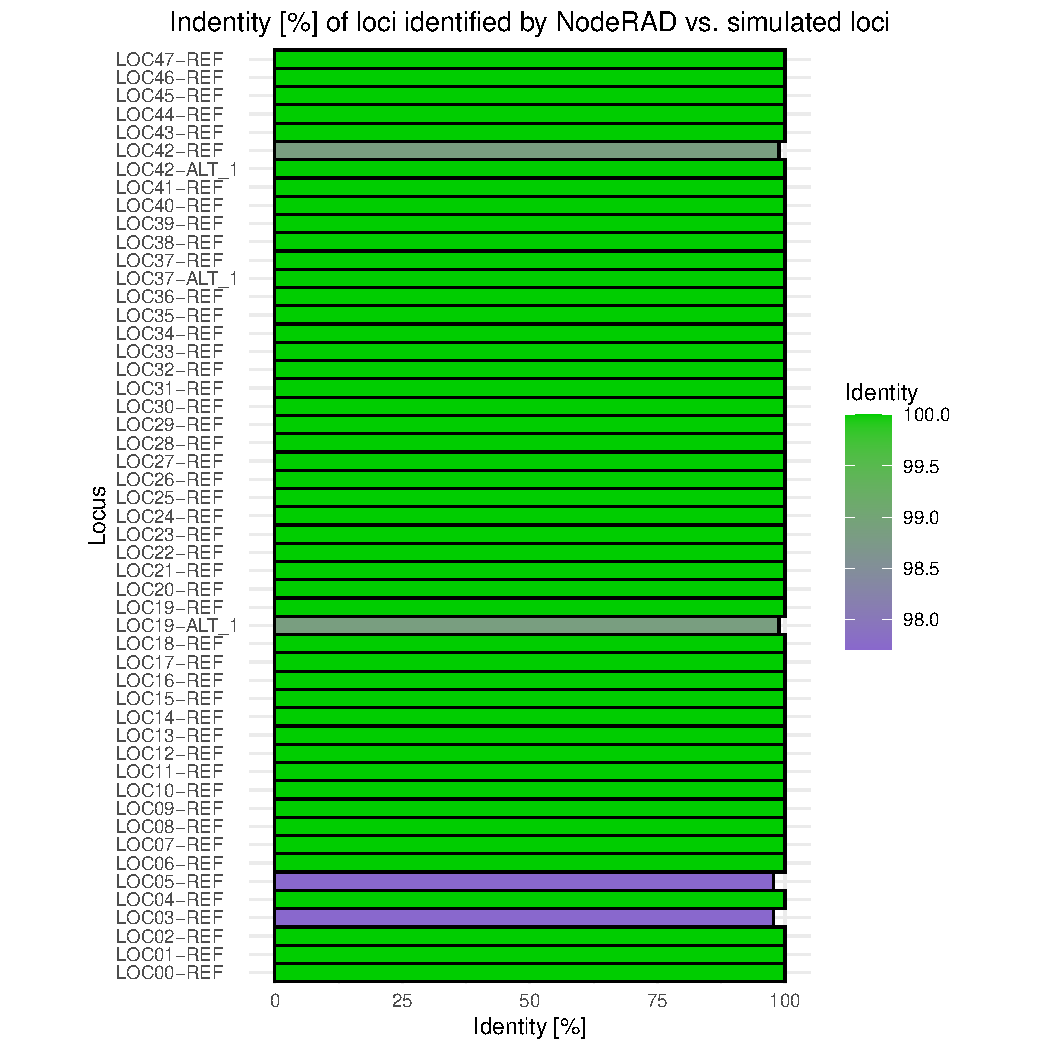
\includegraphics[width=\linewidth]{bilder/evaluation/perc_ident/B.plot_loci.pdf}}
%	\centering{Individuum B.}
%	\end{minipage}
%	\begin{minipage}[b]{.49\linewidth}
%	\subfigure{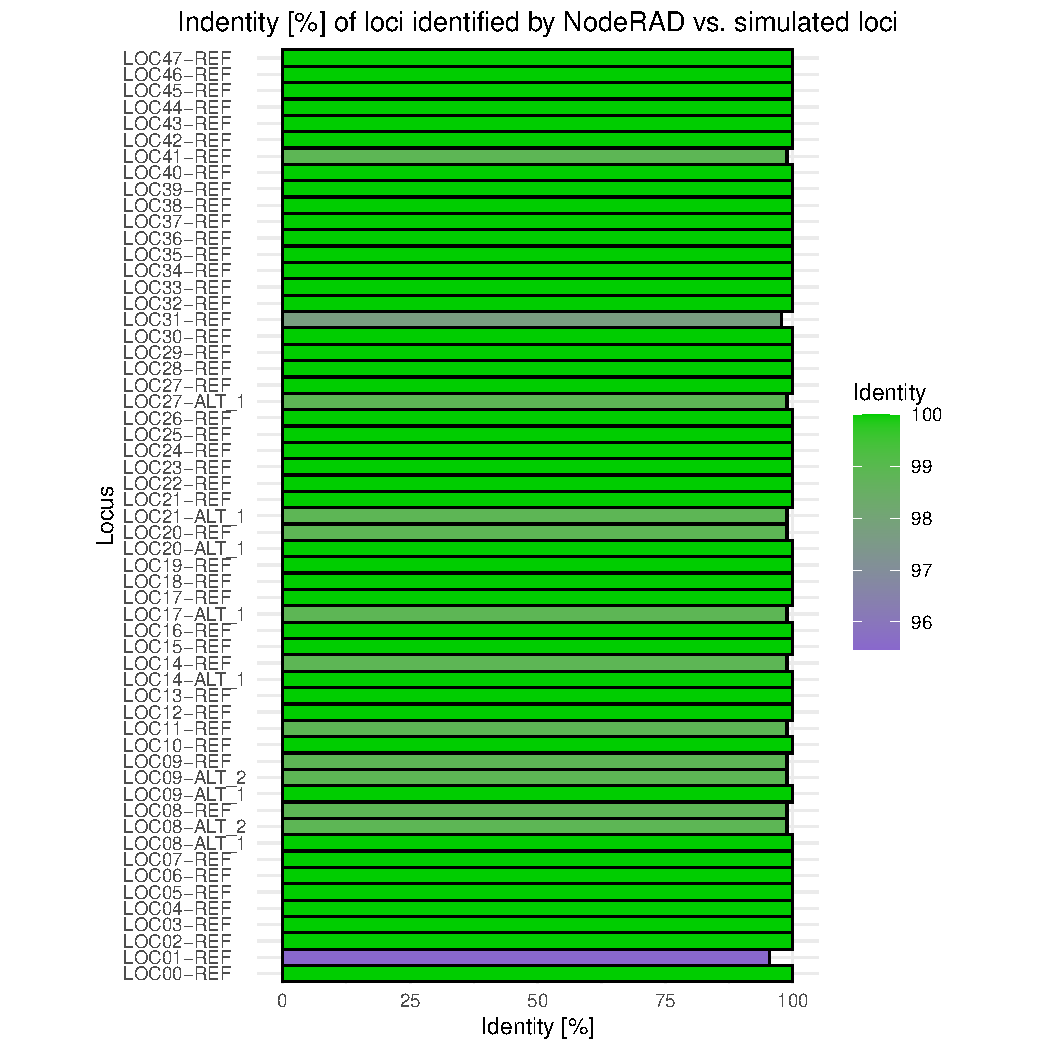
\includegraphics[width=\linewidth]{bilder/evaluation/perc_ident/C.plot_loci.pdf}}
%	\centering{Individuum C.}
%	\end{minipage}
%	\caption{{Sequenzähnlichkeit der durch NodeRAD bestimmten Loci gegenüber den simulierten Loci}}
%	\label{fig:ident_B_C}
%\end{figure}

\begin{figure}[H]
	\begin{center}
		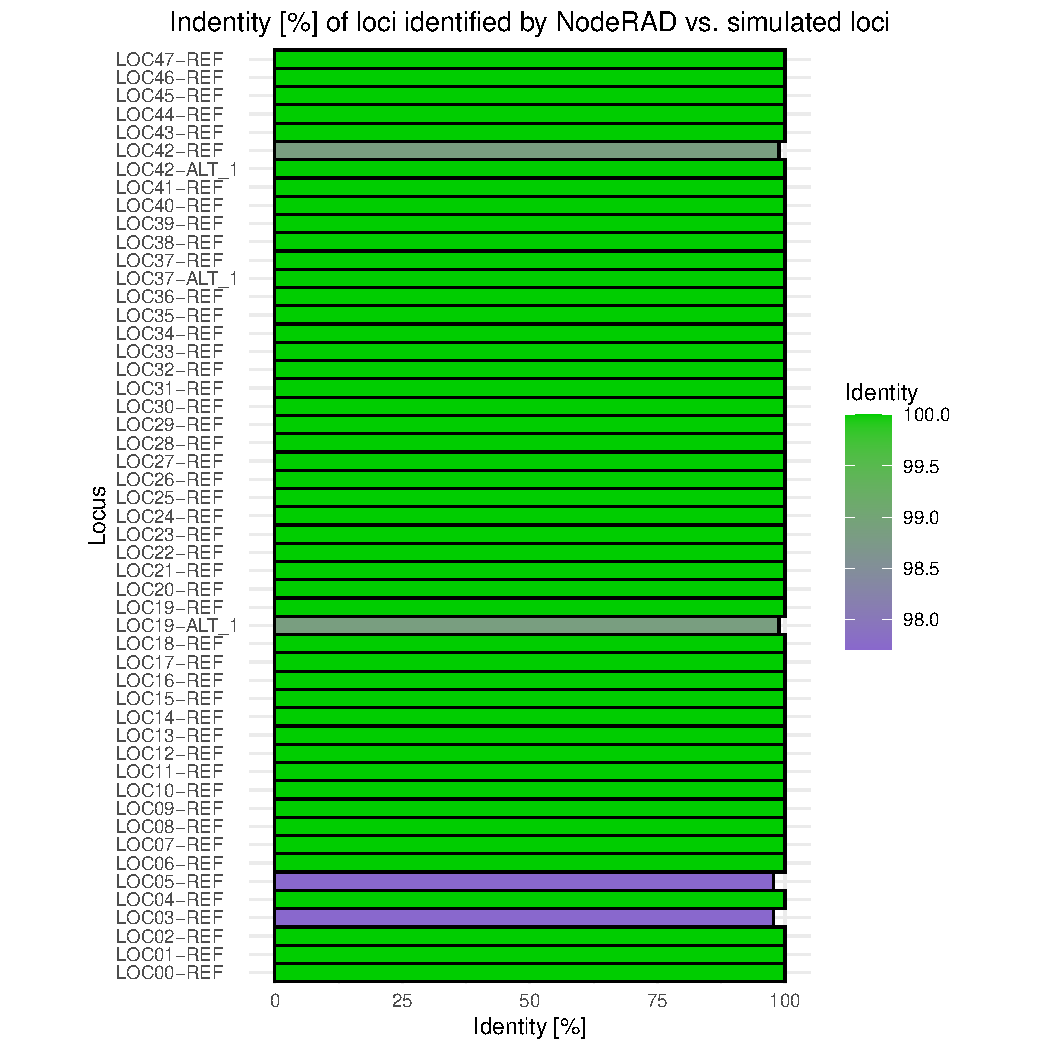
\includegraphics[height=16cm]{bilder/evaluation/perc_ident/B.plot_loci.pdf}
		\caption{Individuum B: Sequenzähnlichkeit (Identität in $ \% $) der durch NodeRAD bestimmten Allele gegenüber den simulierten Allelen.}
	\end{center}
\end{figure}

\begin{figure}[H]
	\begin{center}
		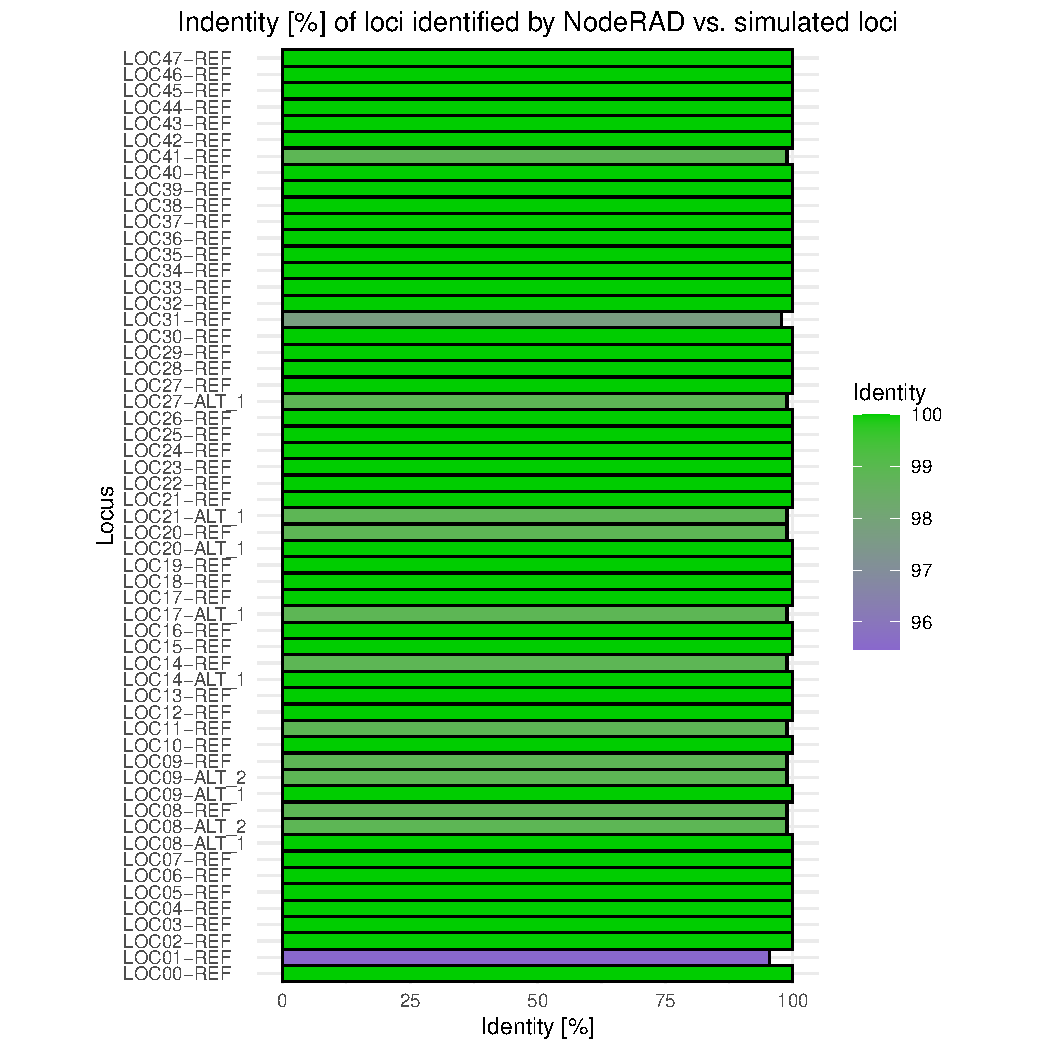
\includegraphics[height=16cm]{bilder/evaluation/perc_ident/C.plot_loci.pdf}
		\caption{Individuum C: Sequenzähnlichkeit (Identität in $ \% $) der durch NodeRAD bestimmten Allele gegenüber den simulierten Allelen.}
	\end{center}
\end{figure}

\begin{figure}[H]
	\begin{center}
		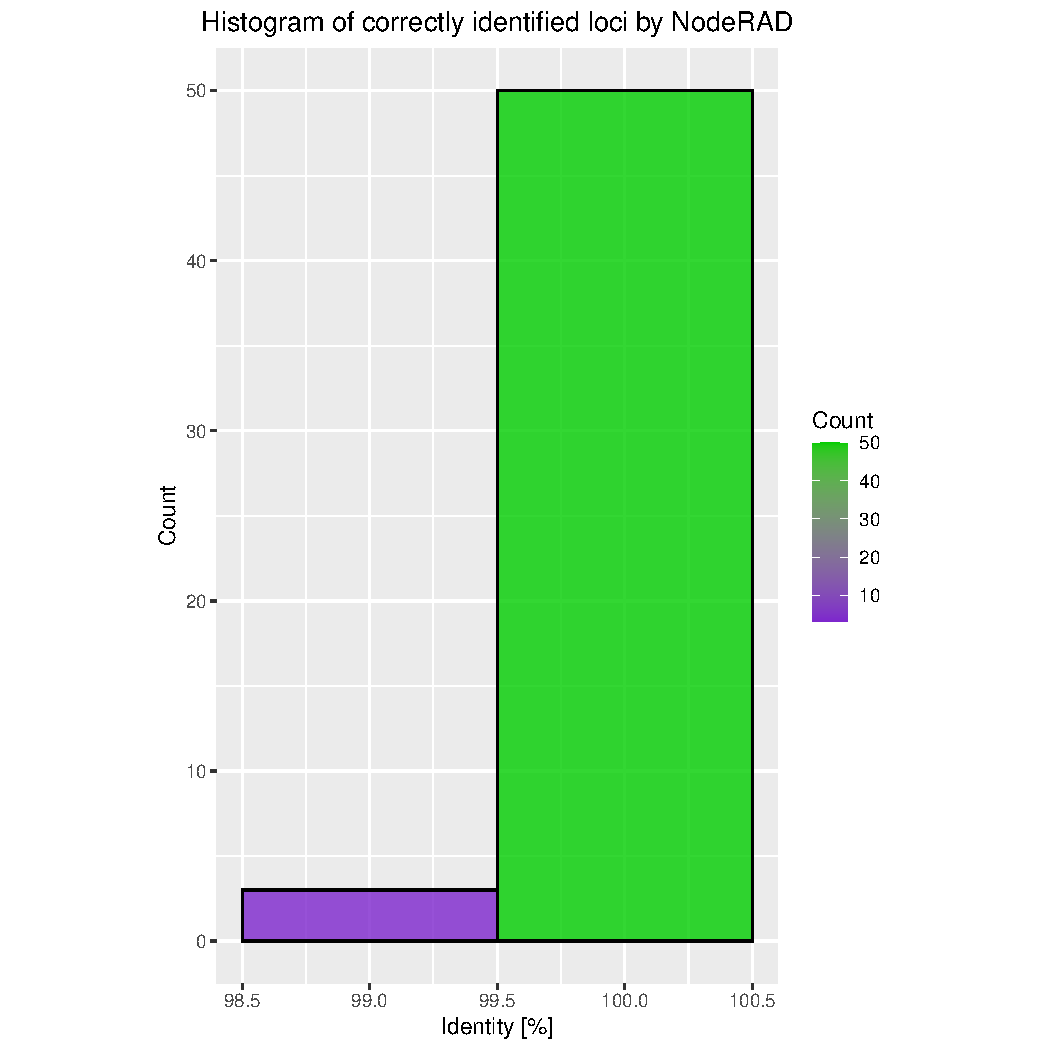
\includegraphics[height=16cm]{bilder/evaluation/hist_perc_ident/B.plot_hist.pdf}
		\caption{Individuum B: Anzahl der durch NodeRAD bestimmten Referenz- und Alternativallele (Spalten REF und ALT in der VCF-Datei) hinsichtlich der Sequenzählichkeit (Identität in $ \% $) zu den simulierten Allelen}
	\end{center}
\end{figure}

\begin{figure}[H]
	\begin{center}
		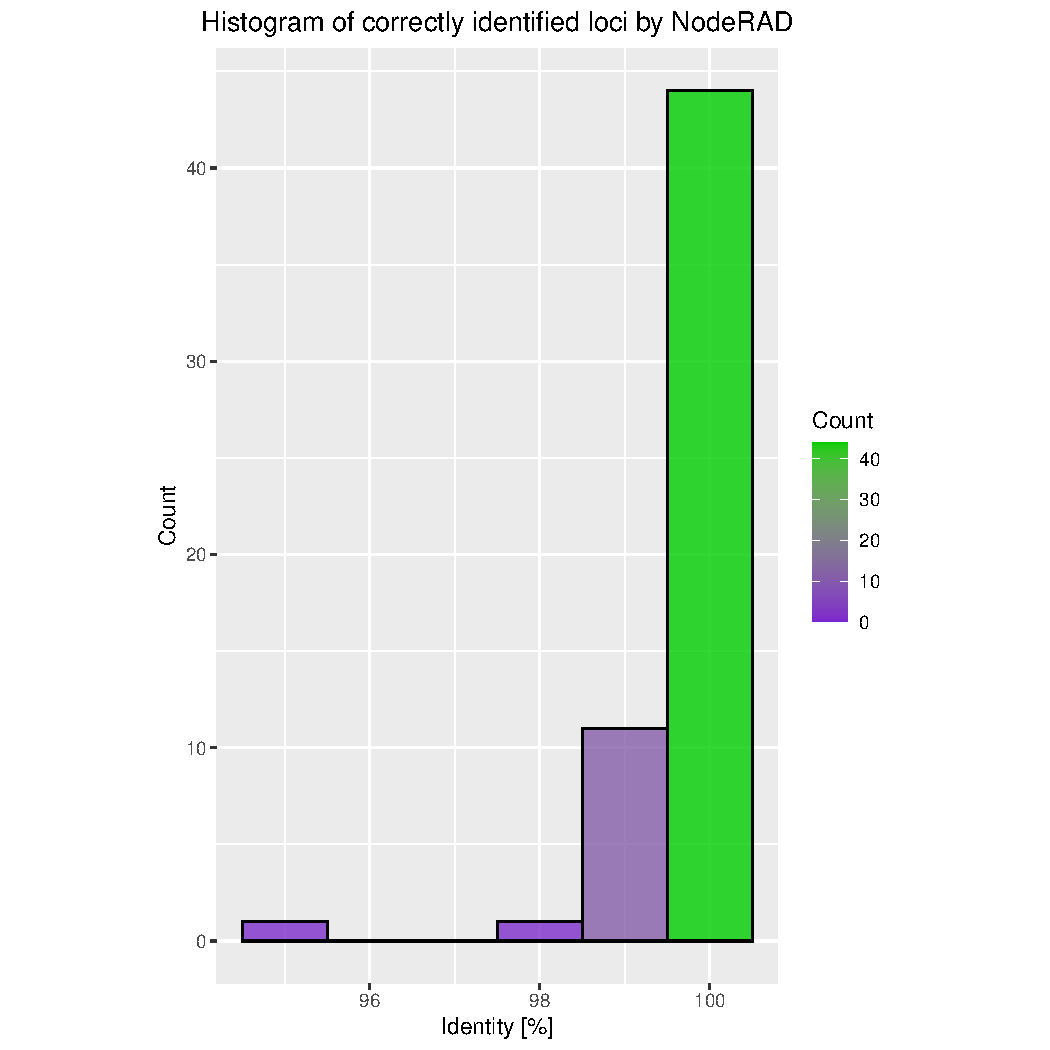
\includegraphics[height=16cm]{bilder/evaluation/hist_perc_ident/C.plot_hist.pdf}
		\caption{Individuum C: Anzahl der durch NodeRAD bestimmten Referenz- und Alternativallele (Spalten REF und ALT in der VCF-Datei) hinsichtlich der Sequenzählichkeit (Identität in $ \% $) zu den simulierten Allelen}
	\end{center}
\end{figure}

\begin{figure}[H]
	\begin{center}
		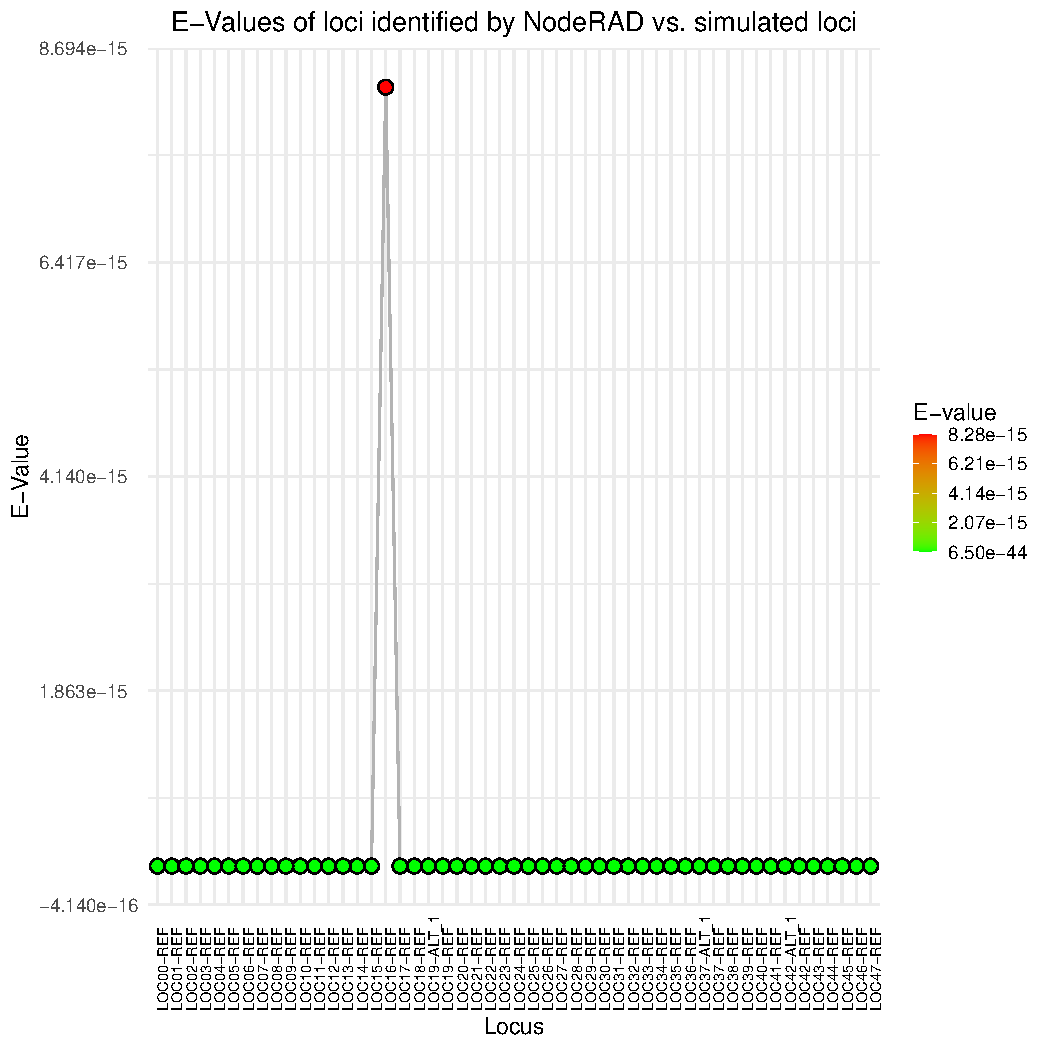
\includegraphics[height=16cm]{bilder/evaluation/evalues/B.plot_evalues.pdf}
		\caption{Individuum B: E-Values aus dem Vergleich der durch NodeRAD bestimmten Loci mit den simulierten Allelen.}
	\end{center}
\end{figure}

\begin{figure}[H]
	\begin{center}
		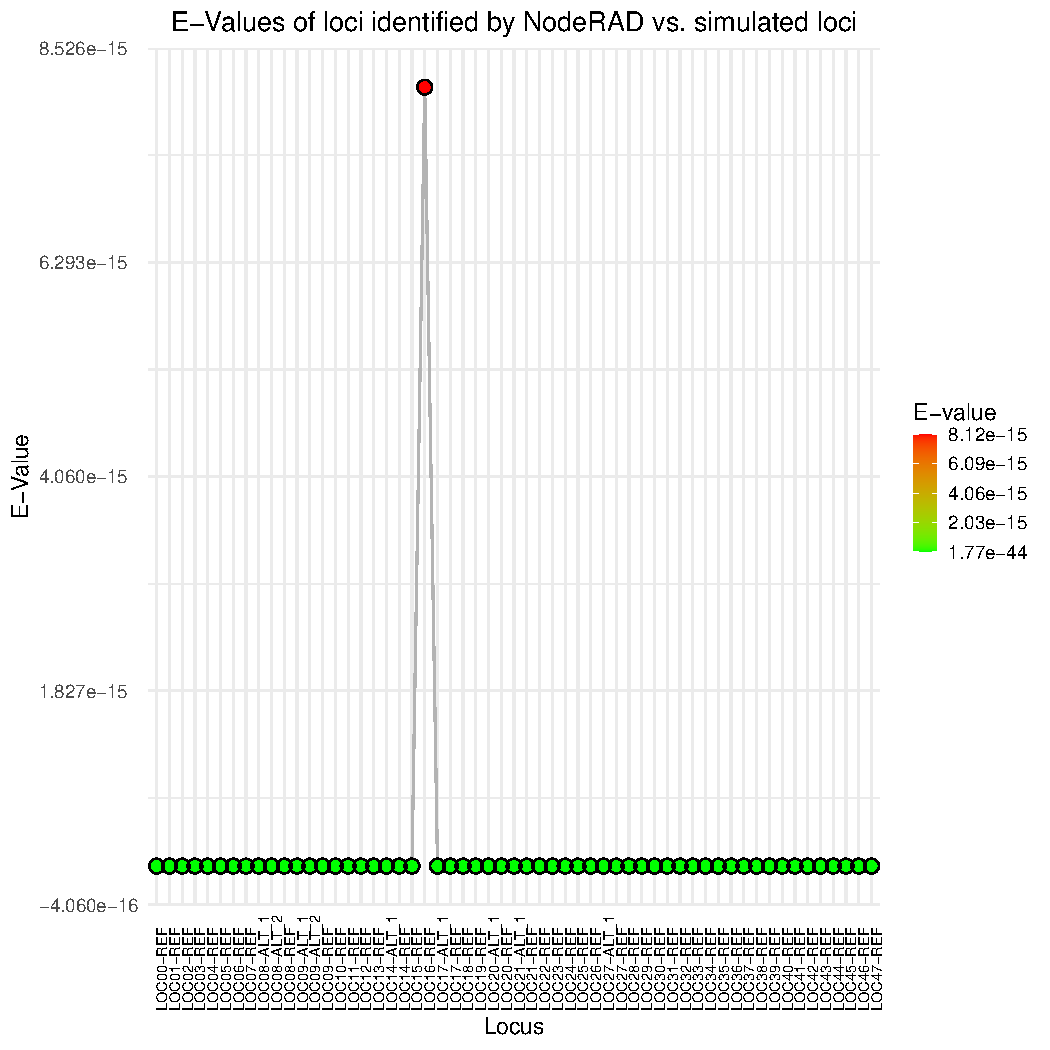
\includegraphics[height=16cm]{bilder/evaluation/evalues/C.plot_evalues.pdf}
		\caption{Individuum C: E-Values aus dem Vergleich der durch NodeRAD bestimmten Allele mit den simulierten Allelen.}
	\end{center}
\end{figure}

\begin{figure}[H]
	\begin{center}
		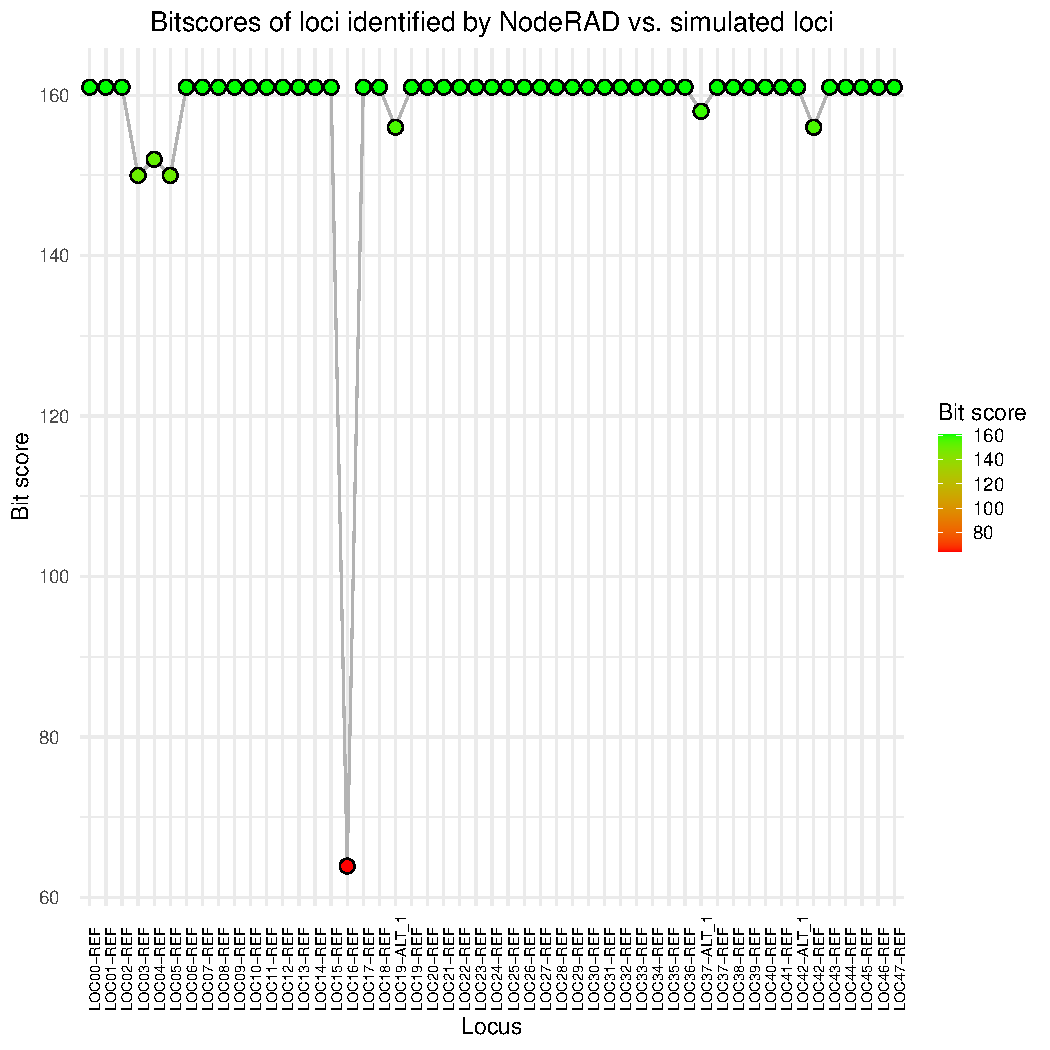
\includegraphics[height=16cm]{bilder/evaluation/bitscores/B.plot_bitscores.pdf}
		\caption{Individuum B: Bitscores aus dem Vergleich der durch NodeRAD bestimmten Allele mit den simulierten Allelen.}
	\end{center}
\end{figure}

\begin{figure}[H]
	\begin{center}
		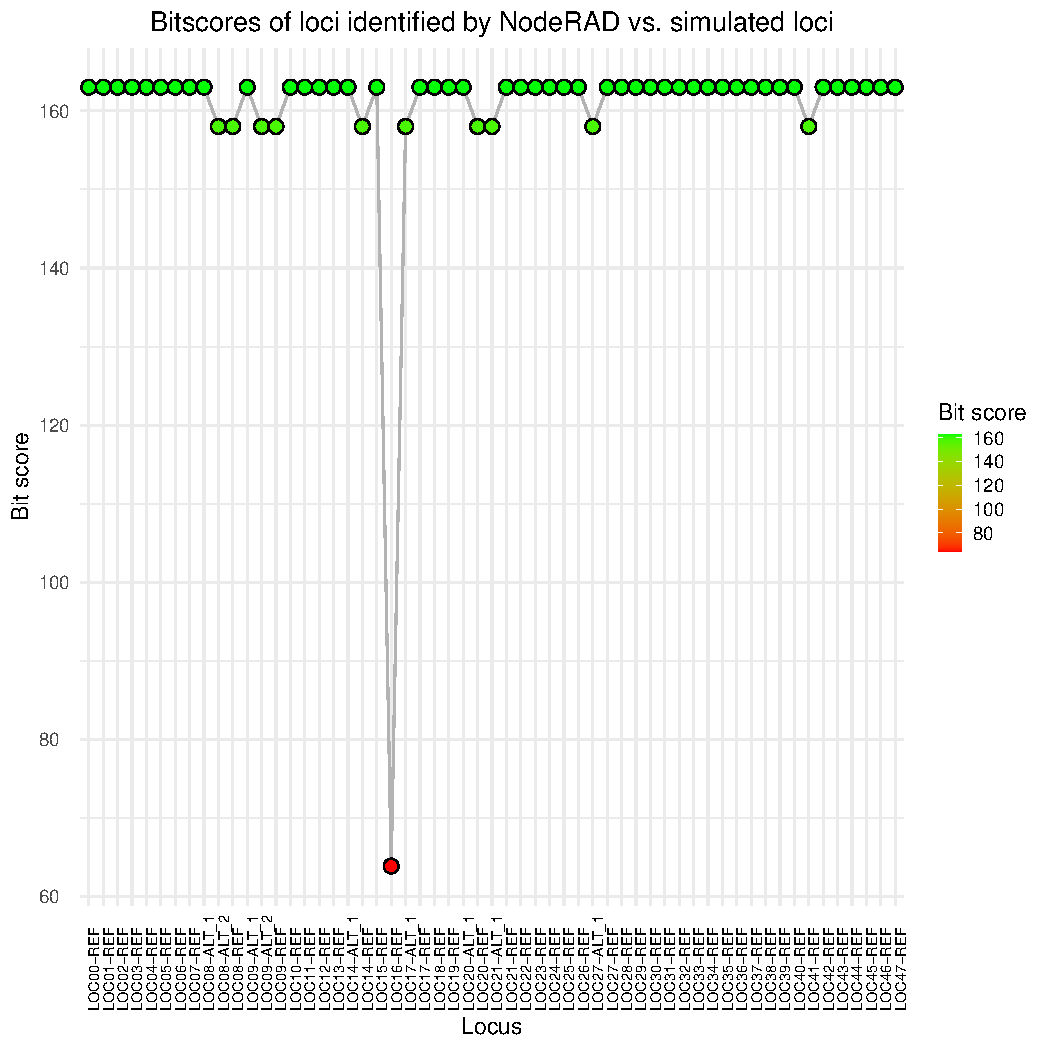
\includegraphics[height=16cm]{bilder/evaluation/bitscores/C.plot_bitscores.pdf}
		\caption{Individuum C: Bitscores aus dem Vergleich der durch NodeRAD bestimmten Allele mit den simulierten Allelen.}
	\end{center}
\end{figure}

\cleardoublepage
% Abbildungsverzeichnis
\listoffigures
\addcontentsline{toc}{chapter}{Abbildungsverzeichnis}
\cleardoublepage
% Algorithmenverzeichnis
\listofalgorithms
\addcontentsline{toc}{chapter}{Algorithmenverzeichnis}
\cleardoublepage
% Literaturverzeichnis
% \bibliographystyle{gerplain}
\bibliographystyle{gerunsrt} % Literaturverzeichnis wird in der Reihenfolge der Zitate im Text aufgebaut
\bibliography{literatur/diplom}
\addcontentsline{toc}{chapter}{\bibname}
% Erklaerung
\thispagestyle{myheadings}
\markboth{}{ERKLÄRUNG}
\addcontentsline{toc}{chapter}{Eidestattliche Versicherung}
% erklaerung.tex
\cleardoublepage
\normalsize
Hiermit versichere ich, dass ich die vorliegende Arbeit selbstständig verfasst habe und keine anderen als die angegebenen Quellen und Hilfsmittel verwendet sowie Zitate kenntlich gemacht habe.\\\\
Dortmund, den \today \\\\\\\\
Muster Mustermann
% EOF
\cleardoublepage
\end{document}

